

\section{About the Braid Group}


\begin{enumerate}
\item Convince yourself geometrically that the defining relations of the braid group on $M$ particles $B_{M}$ are:\begin{equation}
\begin{array}{ r l r }
\sigma _{i} \sigma _{i+1} \sigma _{i} & =\sigma _{i+1} \sigma _{i} \sigma _{i+1} & 1\leq i\leq M-2\\
\sigma _{i} \sigma _{j} & =\sigma _{j} \sigma _{i}\text{ for } \ \ |i-j| >1, & 1\leq i,j\leq M-1
\end{array}
\label{eq:definingRelationsOfBraidGroup}
\end{equation}
\item Instead of thinking about particles on a plane, let us think about particles on the surface of a sphere. In this case, the braid group of $M$ strands on the sphere is written as $B_{M} (S^{2} )$. To think about braids on a sphere, it is useful to think of time as being the radial direction of the sphere, so that braids are drawn as in Fig.\ref{fig:anElementOfBraidGroup}.

\begin{figure}[h!]
\centering
\tikzset {_drkenvclc/.code = {\pgfsetadditionalshadetransform{ \pgftransformshift{\pgfpoint{0 bp } { 0 bp }  }  \pgftransformrotate{-135 }  \pgftransformscale{2 }  }}}
\pgfdeclarehorizontalshading{_rco3hamyb}{150bp}{rgb(0bp)=(0.82,0.89,0.97);
rgb(37.5bp)=(0.82,0.89,0.97);
rgb(43.5bp)=(0.45,0.69,0.91);
rgb(50bp)=(0.29,0.56,0.89);
rgb(57.25bp)=(0.33,0.62,0.88);
rgb(62.5bp)=(0.53,0.74,0.92);
rgb(100bp)=(0.53,0.74,0.92)}
\tikzset{_xjmm1mbdg/.code = {\pgfsetadditionalshadetransform{\pgftransformshift{\pgfpoint{0 bp } { 0 bp }  }  \pgftransformrotate{-135 }  \pgftransformscale{2 } }}}
\pgfdeclarehorizontalshading{_klvb1tza9} {150bp} {color(0bp)=(transparent!0);
color(37.5bp)=(transparent!0);
color(43.5bp)=(transparent!0);
color(50bp)=(transparent!24);
color(57.25bp)=(transparent!0);
color(62.5bp)=(transparent!0);
color(100bp)=(transparent!0) } 
\pgfdeclarefading{_eerx5ge0a}{\tikz \fill[shading=_klvb1tza9,_xjmm1mbdg] (0,0) rectangle (50bp,50bp); } 
\tikzset{every picture/.style={line width=0.75pt}} %set default line width to 0.75pt        

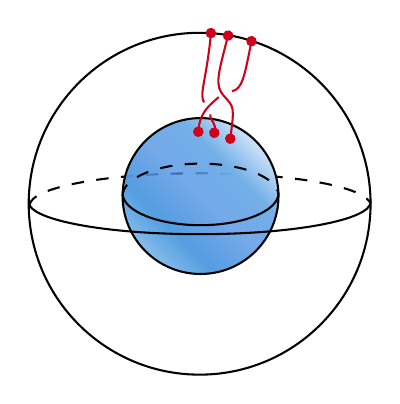
\begin{tikzpicture}[x=0.75pt,y=0.75pt,yscale=-1,xscale=1]
%uncomment if require: \path (0,173); %set diagram left start at 0, and has height of 173

%Shape: Arc [id:dp5560012565025749] 
\draw  [draw opacity=0][dash pattern={on 4.5pt off 4.5pt}] (248.47,86.46) .. controls (248.46,86.35) and (248.46,86.25) .. (248.46,86.14) .. controls (248.46,77.6) and (285.22,70.67) .. (330.58,70.67) .. controls (372.84,70.67) and (407.65,76.69) .. (412.2,84.42) -- (330.58,86.14) -- cycle ; \draw  [dash pattern={on 4.5pt off 4.5pt}] (248.47,86.46) .. controls (248.46,86.35) and (248.46,86.25) .. (248.46,86.14) .. controls (248.46,77.6) and (285.22,70.67) .. (330.58,70.67) .. controls (372.84,70.67) and (407.65,76.69) .. (412.2,84.42) ;  
%Shape: Ellipse [id:dp4263698048259623] 
\path  [shading=_rco3hamyb,_drkenvclc,path fading= _eerx5ge0a ,fading transform={xshift=2}] (293.23,81.65) .. controls (293.23,60.9) and (310.04,44.09) .. (330.78,44.09) .. controls (351.53,44.09) and (368.34,60.9) .. (368.34,81.65) .. controls (368.34,102.39) and (351.53,119.2) .. (330.78,119.2) .. controls (310.04,119.2) and (293.23,102.39) .. (293.23,81.65) -- cycle ; % for fading 
 \draw   (293.23,81.65) .. controls (293.23,60.9) and (310.04,44.09) .. (330.78,44.09) .. controls (351.53,44.09) and (368.34,60.9) .. (368.34,81.65) .. controls (368.34,102.39) and (351.53,119.2) .. (330.78,119.2) .. controls (310.04,119.2) and (293.23,102.39) .. (293.23,81.65) -- cycle ; % for border 

%Shape: Ellipse [id:dp3080229375817509] 
\draw  [color={rgb, 255:red, 0; green, 0; blue, 0 }  ,draw opacity=1 ] (248,85.35) .. controls (248,39.87) and (284.87,3) .. (330.35,3) .. controls (375.83,3) and (412.7,39.87) .. (412.7,85.35) .. controls (412.7,130.83) and (375.83,167.7) .. (330.35,167.7) .. controls (284.87,167.7) and (248,130.83) .. (248,85.35) -- cycle ;
%Shape: Arc [id:dp37808278352551716] 
\draw  [draw opacity=0] (368.34,80.07) .. controls (368.34,80.12) and (368.34,80.17) .. (368.34,80.22) .. controls (368.34,88.76) and (351.52,95.69) .. (330.76,95.69) .. controls (310.65,95.69) and (294.23,89.18) .. (293.22,81.01) -- (330.76,80.22) -- cycle ; \draw   (368.34,80.07) .. controls (368.34,80.12) and (368.34,80.17) .. (368.34,80.22) .. controls (368.34,88.76) and (351.52,95.69) .. (330.76,95.69) .. controls (310.65,95.69) and (294.23,89.18) .. (293.22,81.01) ;  
%Shape: Arc [id:dp6092650545329237] 
\draw  [draw opacity=0][dash pattern={on 4.5pt off 4.5pt}] (293.23,81.65) .. controls (293.22,81.6) and (293.22,81.55) .. (293.22,81.5) .. controls (293.22,72.96) and (310.05,66.03) .. (330.81,66.03) .. controls (350.92,66.03) and (367.34,72.53) .. (368.34,80.71) -- (330.81,81.5) -- cycle ; \draw  [dash pattern={on 4.5pt off 4.5pt}] (293.23,81.65) .. controls (293.22,81.6) and (293.22,81.55) .. (293.22,81.5) .. controls (293.22,72.96) and (310.05,66.03) .. (330.81,66.03) .. controls (350.92,66.03) and (367.34,72.53) .. (368.34,80.71) ;  
%Curve Lines [id:da796477102134888] 
\draw [color={rgb, 255:red, 208; green, 2; blue, 27 }  ,draw opacity=1 ]   (344.05,4.35) .. controls (339.14,23.31) and (337.44,28.43) .. (342.13,33.55) .. controls (346.82,38.67) and (347.25,38.24) .. (345.11,54.03) ;
\draw [shift={(345.11,54.03)}, rotate = 97.7] [color={rgb, 255:red, 208; green, 2; blue, 27 }  ,draw opacity=1 ][fill={rgb, 255:red, 208; green, 2; blue, 27 }  ,fill opacity=1 ][line width=0.75]      (0, 0) circle [x radius= 2.01, y radius= 2.01]   ;
\draw [shift={(344.05,4.35)}, rotate = 104.5] [color={rgb, 255:red, 208; green, 2; blue, 27 }  ,draw opacity=1 ][fill={rgb, 255:red, 208; green, 2; blue, 27 }  ,fill opacity=1 ][line width=0.75]      (0, 0) circle [x radius= 2.01, y radius= 2.01]   ;
%Curve Lines [id:da029436986697203293] 
\draw [color={rgb, 255:red, 208; green, 2; blue, 27 }  ,draw opacity=1 ]   (355.31,7.04) .. controls (351.87,24.6) and (350.88,30.01) .. (345.96,31.16) ;
\draw [shift={(355.31,7.04)}, rotate = 101.1] [color={rgb, 255:red, 208; green, 2; blue, 27 }  ,draw opacity=1 ][fill={rgb, 255:red, 208; green, 2; blue, 27 }  ,fill opacity=1 ][line width=0.75]      (0, 0) circle [x radius= 2.01, y radius= 2.01]   ;
%Curve Lines [id:da6623924253474924] 
\draw [color={rgb, 255:red, 208; green, 2; blue, 27 }  ,draw opacity=1 ]   (339.56,33.95) .. controls (335.62,37.56) and (330.21,41) .. (329.72,50.68) ;
\draw [shift={(329.72,50.68)}, rotate = 92.91] [color={rgb, 255:red, 208; green, 2; blue, 27 }  ,draw opacity=1 ][fill={rgb, 255:red, 208; green, 2; blue, 27 }  ,fill opacity=1 ][line width=0.75]      (0, 0) circle [x radius= 2.01, y radius= 2.01]   ;
%Curve Lines [id:da4988134883638571] 
\draw [color={rgb, 255:red, 208; green, 2; blue, 27 }  ,draw opacity=1 ]   (335.79,3.13) .. controls (333.82,25.25) and (329.88,32.8) .. (332.51,36.57) ;
\draw [shift={(335.79,3.13)}, rotate = 95.09] [color={rgb, 255:red, 208; green, 2; blue, 27 }  ,draw opacity=1 ][fill={rgb, 255:red, 208; green, 2; blue, 27 }  ,fill opacity=1 ][line width=0.75]      (0, 0) circle [x radius= 2.01, y radius= 2.01]   ;
%Curve Lines [id:da69978170330477] 
\draw [color={rgb, 255:red, 208; green, 2; blue, 27 }  ,draw opacity=1 ]   (335.46,42.31) .. controls (335.46,46.25) and (338.74,45.92) .. (337.43,51.17) ;
\draw [shift={(337.43,51.17)}, rotate = 104.04] [color={rgb, 255:red, 208; green, 2; blue, 27 }  ,draw opacity=1 ][fill={rgb, 255:red, 208; green, 2; blue, 27 }  ,fill opacity=1 ][line width=0.75]      (0, 0) circle [x radius= 2.01, y radius= 2.01]   ;
%Shape: Arc [id:dp9702924736551024] 
\draw  [draw opacity=0] (412.68,84.24) .. controls (412.7,84.35) and (412.7,84.45) .. (412.7,84.56) .. controls (412.7,93.1) and (375.82,100.03) .. (330.33,100.03) .. controls (287.94,100.03) and (253.04,94.02) .. (248.46,86.29) -- (330.33,84.56) -- cycle ; \draw   (412.68,84.24) .. controls (412.7,84.35) and (412.7,84.45) .. (412.7,84.56) .. controls (412.7,93.1) and (375.82,100.03) .. (330.33,100.03) .. controls (287.94,100.03) and (253.04,94.02) .. (248.46,86.29) ;  
\end{tikzpicture}
\caption{An element of the braid group $B_{3} (S^{2} )$. The braid shown here is $\sigma _{1} \sigma _{2}^{-1}$}
\label{fig:anElementOfBraidGroup}
\end{figure}

The braid generators on the sphere still obey \eqref{eq:definingRelationsOfBraidGroup}, but they also obey one additional identity\begin{equation}
\sigma _{1} \sigma _{2} \dotsc \sigma _{M-2} \sigma _{M-1} \sigma _{M-1} \sigma _{M-2} \dotsc \sigma _{2} \sigma _{1} =I
\label{eq:definingRelationOfBraidGroupOnSphere}
\end{equation}where $I$ is the identity (or trivial) braid. What does this additional identity mean geometrically? [In fact, for understanding the properties of anyons on a sphere,\eqref{eq:definingRelationOfBraidGroupOnSphere} is not quite enough. We will try to figure out below why this is so by using Ising Anyons as an example.]
\end{enumerate}

\paragraph{Answer}
The second one of \eqref{eq:definingRelationsOfBraidGroup} is trivial, while the first one is due to the Yang-Baxter equation. Take $B_{3}$ for example, the relation $\sigma _{1} \sigma _{2} \sigma _{1} =\sigma _{2} \sigma _{1} \sigma _{2}$ equals to Fig.\ref{fig:YangBaxterConfiguration}.
\begin{figure}[h!]
\centering
\tikzset{every picture/.style={line width=0.75pt}} %set default line width to 0.75pt        

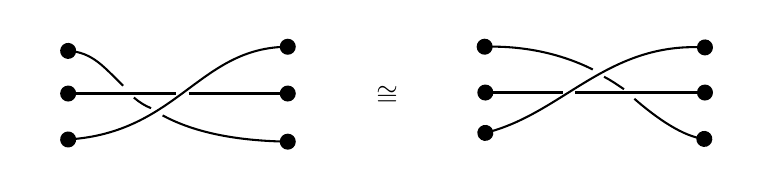
\begin{tikzpicture}[x=0.75pt,y=0.75pt,yscale=-1,xscale=1]
%uncomment if require: \path (0,77); %set diagram left start at 0, and has height of 77

%Curve Lines [id:da4695897073733857] 
\draw    (209.67,39.67) .. controls (212.24,41.95) and (215.1,43.67) .. (217.95,44.81) ;
%Curve Lines [id:da5647335848772184] 
\draw    (436.2,29.67) .. controls (439.4,31.27) and (442.15,33.24) .. (445.8,35.67) ;
%Curve Lines [id:da011650194585989482] 
\draw    (450.8,40.27) .. controls (461.63,49.7) and (474.5,58.61) .. (484.5,59.61) ;
\draw [shift={(484.5,59.61)}, rotate = 5.71] [color={rgb, 255:red, 0; green, 0; blue, 0 }  ][fill={rgb, 255:red, 0; green, 0; blue, 0 }  ][line width=0.75]      (0, 0) circle [x radius= 3.35, y radius= 3.35]   ;
%Curve Lines [id:da10622734266529665] 
\draw    (378.67,15.18) .. controls (400.5,14.61) and (417.98,19.77) .. (430.78,26.17) ;
\draw [shift={(378.67,15.18)}, rotate = 358.51] [color={rgb, 255:red, 0; green, 0; blue, 0 }  ][fill={rgb, 255:red, 0; green, 0; blue, 0 }  ][line width=0.75]      (0, 0) circle [x radius= 3.35, y radius= 3.35]   ;


% Text Node
\draw (159,7) node [anchor=north west][inner sep=0.75pt]    {$\ $};
% Text Node
\draw (291.81,7) node [anchor=north west][inner sep=0.75pt]    {$\ $};
% Text Node
\draw (159,30.74) node [anchor=north west][inner sep=0.75pt]    {$\ $};
% Text Node
\draw (291.81,30.74) node [anchor=north west][inner sep=0.75pt]    {$\ $};
% Text Node
\draw (159,54.49) node [anchor=north west][inner sep=0.75pt]    {$\ $};
% Text Node
\draw (291.81,54.49) node [anchor=north west][inner sep=0.75pt]    {$\ $};
% Text Node
\draw (360,6.51) node [anchor=north west][inner sep=0.75pt]    {$\ $};
% Text Node
\draw (492.81,8.51) node [anchor=north west][inner sep=0.75pt]    {$\ $};
% Text Node
\draw (360,30.26) node [anchor=north west][inner sep=0.75pt]    {$\ $};
% Text Node
\draw (492.81,30.26) node [anchor=north west][inner sep=0.75pt]    {$\ $};
% Text Node
\draw (360,54) node [anchor=north west][inner sep=0.75pt]    {$\ $};
% Text Node
\draw (492.81,54) node [anchor=north west][inner sep=0.75pt]    {$\ $};
% Text Node
\draw (325,33) node [anchor=north west][inner sep=0.75pt]    {$\cong $};
% Connection
\draw    (178,37.74) -- (230.02,37.74)(236.02,37.74) -- (283.81,37.74) ;
\draw [shift={(283.81,37.74)}, rotate = 0] [color={rgb, 255:red, 0; green, 0; blue, 0 }  ][fill={rgb, 255:red, 0; green, 0; blue, 0 }  ][line width=0.75]      (0, 0) circle [x radius= 3.35, y radius= 3.35]   ;
\draw [shift={(178,37.74)}, rotate = 0] [color={rgb, 255:red, 0; green, 0; blue, 0 }  ][fill={rgb, 255:red, 0; green, 0; blue, 0 }  ][line width=0.75]      (0, 0) circle [x radius= 3.35, y radius= 3.35]   ;
% Connection
\draw    (178,59.88) .. controls (231,56.5) and (241,15.5) .. (283.81,15.2) ;
\draw [shift={(283.81,15.2)}, rotate = 359.61] [color={rgb, 255:red, 0; green, 0; blue, 0 }  ][fill={rgb, 255:red, 0; green, 0; blue, 0 }  ][line width=0.75]      (0, 0) circle [x radius= 3.35, y radius= 3.35]   ;
\draw [shift={(178,59.88)}, rotate = 356.35] [color={rgb, 255:red, 0; green, 0; blue, 0 }  ][fill={rgb, 255:red, 0; green, 0; blue, 0 }  ][line width=0.75]      (0, 0) circle [x radius= 3.35, y radius= 3.35]   ;
% Connection
\draw    (178,17.2) .. controls (189.76,17.74) and (195.52,25.29) .. (204.46,33.97)(223.51,48.28) .. controls (236.15,55.07) and (254.48,60.42) .. (283.81,60.93) ;
\draw [shift={(283.81,60.93)}, rotate = 0.98] [color={rgb, 255:red, 0; green, 0; blue, 0 }  ][fill={rgb, 255:red, 0; green, 0; blue, 0 }  ][line width=0.75]      (0, 0) circle [x radius= 3.35, y radius= 3.35]   ;
\draw [shift={(178,17.2)}, rotate = 2.64] [color={rgb, 255:red, 0; green, 0; blue, 0 }  ][fill={rgb, 255:red, 0; green, 0; blue, 0 }  ][line width=0.75]      (0, 0) circle [x radius= 3.35, y radius= 3.35]   ;
% Connection
\draw    (379,37.26) -- (416.21,37.26)(422.21,37.26) -- (484.81,37.26) ;
\draw [shift={(484.81,37.26)}, rotate = 0] [color={rgb, 255:red, 0; green, 0; blue, 0 }  ][fill={rgb, 255:red, 0; green, 0; blue, 0 }  ][line width=0.75]      (0, 0) circle [x radius= 3.35, y radius= 3.35]   ;
\draw [shift={(379,37.26)}, rotate = 0] [color={rgb, 255:red, 0; green, 0; blue, 0 }  ][fill={rgb, 255:red, 0; green, 0; blue, 0 }  ][line width=0.75]      (0, 0) circle [x radius= 3.35, y radius= 3.35]   ;
% Connection
\draw    (379,56.71) .. controls (416.29,47.49) and (437.61,12.81) .. (484.81,15.53) ;
\draw [shift={(484.81,15.53)}, rotate = 3.3] [color={rgb, 255:red, 0; green, 0; blue, 0 }  ][fill={rgb, 255:red, 0; green, 0; blue, 0 }  ][line width=0.75]      (0, 0) circle [x radius= 3.35, y radius= 3.35]   ;
\draw [shift={(379,56.71)}, rotate = 346.11] [color={rgb, 255:red, 0; green, 0; blue, 0 }  ][fill={rgb, 255:red, 0; green, 0; blue, 0 }  ][line width=0.75]      (0, 0) circle [x radius= 3.35, y radius= 3.35]   ;

\end{tikzpicture}
\caption{The configuration of  $\sigma _{1} \sigma _{2} \sigma _{1} =\sigma _{2} \sigma _{1} \sigma _{2}$.}
\label{fig:YangBaxterConfiguration}
\end{figure}

(b) We also take $B_{3} (S^{2} )$ for example. Relation \eqref{eq:definingRelationOfBraidGroupOnSphere} now becomes
\begin{equation*}
\sigma _{1} \sigma _{2} \sigma _{2} \sigma _{1} =I,
\end{equation*}
here we define $\sigma _{1}$ to be as Fig.\ref{fig:sigma1OnSphere} shows. 
\begin{figure}[h!]
\centering
\tikzset {_9fxpz3bxq/.code = {\pgfsetadditionalshadetransform{ \pgftransformshift{\pgfpoint{0 bp } { 0 bp }  }  \pgftransformrotate{-135 }  \pgftransformscale{2 }  }}}
\pgfdeclarehorizontalshading{_awrbgw5x1}{150bp}{rgb(0bp)=(0.82,0.89,0.97);
rgb(37.5bp)=(0.82,0.89,0.97);
rgb(43.5bp)=(0.45,0.69,0.91);
rgb(50bp)=(0.29,0.56,0.89);
rgb(57.25bp)=(0.33,0.62,0.88);
rgb(62.5bp)=(0.53,0.74,0.92);
rgb(100bp)=(0.53,0.74,0.92)}
\tikzset{_0vvkgsy6e/.code = {\pgfsetadditionalshadetransform{\pgftransformshift{\pgfpoint{0 bp } { 0 bp }  }  \pgftransformrotate{-135 }  \pgftransformscale{2 } }}}
\pgfdeclarehorizontalshading{_58eq1bn00} {150bp} {color(0bp)=(transparent!0);
color(37.5bp)=(transparent!0);
color(43.5bp)=(transparent!0);
color(50bp)=(transparent!24);
color(57.25bp)=(transparent!0);
color(62.5bp)=(transparent!0);
color(100bp)=(transparent!0) } 
\pgfdeclarefading{_gw0id4ku0}{\tikz \fill[shading=_58eq1bn00,_0vvkgsy6e] (0,0) rectangle (50bp,50bp); } 

% Gradient Info
  
\tikzset {_s7m4689cg/.code = {\pgfsetadditionalshadetransform{ \pgftransformshift{\pgfpoint{0 bp } { 0 bp }  }  \pgftransformrotate{-135 }  \pgftransformscale{2 }  }}}
\pgfdeclarehorizontalshading{_e93ht5hdp}{150bp}{rgb(0bp)=(0.82,0.89,0.97);
rgb(37.5bp)=(0.82,0.89,0.97);
rgb(43.5bp)=(0.45,0.69,0.91);
rgb(50bp)=(0.29,0.56,0.89);
rgb(57.25bp)=(0.33,0.62,0.88);
rgb(62.5bp)=(0.53,0.74,0.92);
rgb(100bp)=(0.53,0.74,0.92)}
\tikzset{_3rjuh681a/.code = {\pgfsetadditionalshadetransform{\pgftransformshift{\pgfpoint{0 bp } { 0 bp }  }  \pgftransformrotate{-135 }  \pgftransformscale{2 } }}}
\pgfdeclarehorizontalshading{_u10png40g} {150bp} {color(0bp)=(transparent!0);
color(37.5bp)=(transparent!0);
color(43.5bp)=(transparent!0);
color(50bp)=(transparent!24);
color(57.25bp)=(transparent!0);
color(62.5bp)=(transparent!0);
color(100bp)=(transparent!0) } 
\pgfdeclarefading{_hw4hhwzvn}{\tikz \fill[shading=_u10png40g,_3rjuh681a] (0,0) rectangle (50bp,50bp); } 
\tikzset{every picture/.style={line width=0.75pt}} %set default line width to 0.75pt        

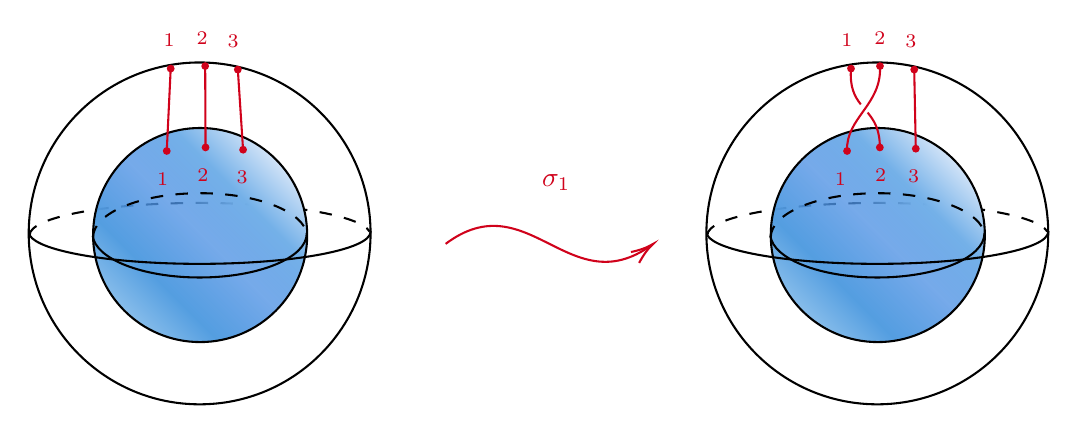
\begin{tikzpicture}[x=0.75pt,y=0.75pt,yscale=-1,xscale=1]
%uncomment if require: \path (0,186); %set diagram left start at 0, and has height of 186

%Shape: Arc [id:dp45382128827395785] 
\draw  [draw opacity=0][dash pattern={on 4.5pt off 4.5pt}] (87.61,104.47) .. controls (87.59,104.37) and (87.59,104.26) .. (87.59,104.16) .. controls (87.59,95.61) and (124.36,88.69) .. (169.71,88.69) .. controls (211.97,88.69) and (246.78,94.7) .. (251.33,102.43) -- (169.71,104.16) -- cycle ; \draw  [dash pattern={on 4.5pt off 4.5pt}] (87.61,104.47) .. controls (87.59,104.37) and (87.59,104.26) .. (87.59,104.16) .. controls (87.59,95.61) and (124.36,88.69) .. (169.71,88.69) .. controls (211.97,88.69) and (246.78,94.7) .. (251.33,102.43) ;  
%Shape: Ellipse [id:dp07766570156663999] 
\path  [shading=_awrbgw5x1,_9fxpz3bxq,path fading= _gw0id4ku0 ,fading transform={xshift=2}] (118.14,104.16) .. controls (118.14,75.67) and (141.23,52.58) .. (169.71,52.58) .. controls (198.2,52.58) and (221.29,75.67) .. (221.29,104.16) .. controls (221.29,132.64) and (198.2,155.73) .. (169.71,155.73) .. controls (141.23,155.73) and (118.14,132.64) .. (118.14,104.16) -- cycle ; % for fading 
 \draw   (118.14,104.16) .. controls (118.14,75.67) and (141.23,52.58) .. (169.71,52.58) .. controls (198.2,52.58) and (221.29,75.67) .. (221.29,104.16) .. controls (221.29,132.64) and (198.2,155.73) .. (169.71,155.73) .. controls (141.23,155.73) and (118.14,132.64) .. (118.14,104.16) -- cycle ; % for border 

%Shape: Ellipse [id:dp2297231392064336] 
\draw  [color={rgb, 255:red, 0; green, 0; blue, 0 }  ,draw opacity=1 ] (87.13,103.37) .. controls (87.13,57.88) and (124,21.01) .. (169.48,21.01) .. controls (214.96,21.01) and (251.83,57.88) .. (251.83,103.37) .. controls (251.83,148.85) and (214.96,185.72) .. (169.48,185.72) .. controls (124,185.72) and (87.13,148.85) .. (87.13,103.37) -- cycle ;
%Shape: Arc [id:dp5627141860911213] 
\draw  [draw opacity=0] (221.09,103.17) .. controls (221.09,103.23) and (221.09,103.3) .. (221.09,103.37) .. controls (221.09,115.1) and (197.99,124.61) .. (169.48,124.61) .. controls (141.87,124.61) and (119.32,115.68) .. (117.94,104.46) -- (169.48,103.37) -- cycle ; \draw   (221.09,103.17) .. controls (221.09,103.23) and (221.09,103.3) .. (221.09,103.37) .. controls (221.09,115.1) and (197.99,124.61) .. (169.48,124.61) .. controls (141.87,124.61) and (119.32,115.68) .. (117.94,104.46) ;  
%Shape: Arc [id:dp01515312917841416] 
\draw  [draw opacity=0][dash pattern={on 4.5pt off 4.5pt}] (118.14,105.45) .. controls (118.14,105.38) and (118.14,105.31) .. (118.14,105.25) .. controls (118.14,93.51) and (141.24,84) .. (169.74,84) .. controls (197.36,84) and (219.91,92.93) .. (221.29,104.16) -- (169.74,105.25) -- cycle ; \draw  [dash pattern={on 4.5pt off 4.5pt}] (118.14,105.45) .. controls (118.14,105.38) and (118.14,105.31) .. (118.14,105.25) .. controls (118.14,93.51) and (141.24,84) .. (169.74,84) .. controls (197.36,84) and (219.91,92.93) .. (221.29,104.16) ;  
%Shape: Arc [id:dp7537832647078875] 
\draw  [draw opacity=0] (251.82,102.26) .. controls (251.83,102.36) and (251.83,102.47) .. (251.83,102.57) .. controls (251.83,111.12) and (214.95,118.04) .. (169.46,118.04) .. controls (127.08,118.04) and (92.17,112.03) .. (87.59,104.3) -- (169.46,102.57) -- cycle ; \draw   (251.82,102.26) .. controls (251.83,102.36) and (251.83,102.47) .. (251.83,102.57) .. controls (251.83,111.12) and (214.95,118.04) .. (169.46,118.04) .. controls (127.08,118.04) and (92.17,112.03) .. (87.59,104.3) ;  

%Shape: Arc [id:dp23596729534619776] 
\draw  [draw opacity=0][dash pattern={on 4.5pt off 4.5pt}] (414.11,104.47) .. controls (414.09,104.37) and (414.09,104.26) .. (414.09,104.16) .. controls (414.09,95.61) and (450.86,88.69) .. (496.21,88.69) .. controls (538.47,88.69) and (573.28,94.7) .. (577.83,102.43) -- (496.21,104.16) -- cycle ; \draw  [dash pattern={on 4.5pt off 4.5pt}] (414.11,104.47) .. controls (414.09,104.37) and (414.09,104.26) .. (414.09,104.16) .. controls (414.09,95.61) and (450.86,88.69) .. (496.21,88.69) .. controls (538.47,88.69) and (573.28,94.7) .. (577.83,102.43) ;  
%Shape: Ellipse [id:dp6128193610723671] 
\path  [shading=_e93ht5hdp,_s7m4689cg,path fading= _hw4hhwzvn ,fading transform={xshift=2}] (444.64,104.16) .. controls (444.64,75.67) and (467.73,52.58) .. (496.21,52.58) .. controls (524.7,52.58) and (547.79,75.67) .. (547.79,104.16) .. controls (547.79,132.64) and (524.7,155.73) .. (496.21,155.73) .. controls (467.73,155.73) and (444.64,132.64) .. (444.64,104.16) -- cycle ; % for fading 
 \draw   (444.64,104.16) .. controls (444.64,75.67) and (467.73,52.58) .. (496.21,52.58) .. controls (524.7,52.58) and (547.79,75.67) .. (547.79,104.16) .. controls (547.79,132.64) and (524.7,155.73) .. (496.21,155.73) .. controls (467.73,155.73) and (444.64,132.64) .. (444.64,104.16) -- cycle ; % for border 

%Shape: Ellipse [id:dp2645593747503847] 
\draw  [color={rgb, 255:red, 0; green, 0; blue, 0 }  ,draw opacity=1 ] (413.63,103.37) .. controls (413.63,57.88) and (450.5,21.01) .. (495.98,21.01) .. controls (541.46,21.01) and (578.33,57.88) .. (578.33,103.37) .. controls (578.33,148.85) and (541.46,185.72) .. (495.98,185.72) .. controls (450.5,185.72) and (413.63,148.85) .. (413.63,103.37) -- cycle ;
%Shape: Arc [id:dp29679710633554346] 
\draw  [draw opacity=0] (547.59,103.17) .. controls (547.59,103.23) and (547.59,103.3) .. (547.59,103.37) .. controls (547.59,115.1) and (524.49,124.61) .. (495.98,124.61) .. controls (468.37,124.61) and (445.82,115.68) .. (444.44,104.46) -- (495.98,103.37) -- cycle ; \draw   (547.59,103.17) .. controls (547.59,103.23) and (547.59,103.3) .. (547.59,103.37) .. controls (547.59,115.1) and (524.49,124.61) .. (495.98,124.61) .. controls (468.37,124.61) and (445.82,115.68) .. (444.44,104.46) ;  
%Shape: Arc [id:dp8598539626103405] 
\draw  [draw opacity=0][dash pattern={on 4.5pt off 4.5pt}] (444.64,105.45) .. controls (444.64,105.38) and (444.64,105.31) .. (444.64,105.25) .. controls (444.64,93.51) and (467.74,84) .. (496.24,84) .. controls (523.86,84) and (546.41,92.93) .. (547.79,104.16) -- (496.24,105.25) -- cycle ; \draw  [dash pattern={on 4.5pt off 4.5pt}] (444.64,105.45) .. controls (444.64,105.38) and (444.64,105.31) .. (444.64,105.25) .. controls (444.64,93.51) and (467.74,84) .. (496.24,84) .. controls (523.86,84) and (546.41,92.93) .. (547.79,104.16) ;  
%Shape: Arc [id:dp9782373223134726] 
\draw  [draw opacity=0] (578.32,102.26) .. controls (578.33,102.36) and (578.33,102.47) .. (578.33,102.57) .. controls (578.33,111.12) and (541.45,118.04) .. (495.96,118.04) .. controls (453.58,118.04) and (418.67,112.03) .. (414.09,104.3) -- (495.96,102.57) -- cycle ; \draw   (578.32,102.26) .. controls (578.33,102.36) and (578.33,102.47) .. (578.33,102.57) .. controls (578.33,111.12) and (541.45,118.04) .. (495.96,118.04) .. controls (453.58,118.04) and (418.67,112.03) .. (414.09,104.3) ;  

%Curve Lines [id:da8981908652043] 
\draw [color={rgb, 255:red, 208; green, 2; blue, 27 }  ,draw opacity=1 ]   (288,108.41) .. controls (327.6,78.71) and (347.6,137.21) .. (386.81,109.28) ;
\draw [shift={(388,108.41)}, rotate = 143.13] [color={rgb, 255:red, 208; green, 2; blue, 27 }  ,draw opacity=1 ][line width=0.75]    (10.93,-3.29) .. controls (6.95,-1.4) and (3.31,-0.3) .. (0,0) .. controls (3.31,0.3) and (6.95,1.4) .. (10.93,3.29)   ;


% Text Node
\draw (333,73.41) node [anchor=north west][inner sep=0.75pt]  [color={rgb, 255:red, 208; green, 2; blue, 27 }  ,opacity=1 ]  {$\sigma _{1}$};
% Text Node
\draw (150.69,5.95) node [anchor=north west][inner sep=0.75pt]  [font=\scriptsize,color={rgb, 255:red, 208; green, 2; blue, 27 }  ,opacity=1 ]  {$1$};
% Text Node
\draw (166.59,4.75) node [anchor=north west][inner sep=0.75pt]  [font=\scriptsize,color={rgb, 255:red, 208; green, 2; blue, 27 }  ,opacity=1 ]  {$2$};
% Text Node
\draw (181.49,6.45) node [anchor=north west][inner sep=0.75pt]  [font=\scriptsize,color={rgb, 255:red, 208; green, 2; blue, 27 }  ,opacity=1 ]  {$3$};
% Text Node
\draw (147.49,72.65) node [anchor=north west][inner sep=0.75pt]  [font=\scriptsize,color={rgb, 255:red, 208; green, 2; blue, 27 }  ,opacity=1 ]  {$1$};
% Text Node
\draw (166.89,70.95) node [anchor=north west][inner sep=0.75pt]  [font=\scriptsize,color={rgb, 255:red, 208; green, 2; blue, 27 }  ,opacity=1 ]  {$2$};
% Text Node
\draw (185.79,72.05) node [anchor=north west][inner sep=0.75pt]  [font=\scriptsize,color={rgb, 255:red, 208; green, 2; blue, 27 }  ,opacity=1 ]  {$3$};
% Text Node
\draw (477.19,5.95) node [anchor=north west][inner sep=0.75pt]  [font=\scriptsize,color={rgb, 255:red, 208; green, 2; blue, 27 }  ,opacity=1 ]  {$1$};
% Text Node
\draw (493.09,4.75) node [anchor=north west][inner sep=0.75pt]  [font=\scriptsize,color={rgb, 255:red, 208; green, 2; blue, 27 }  ,opacity=1 ]  {$2$};
% Text Node
\draw (507.99,6.45) node [anchor=north west][inner sep=0.75pt]  [font=\scriptsize,color={rgb, 255:red, 208; green, 2; blue, 27 }  ,opacity=1 ]  {$3$};
% Text Node
\draw (473.99,72.65) node [anchor=north west][inner sep=0.75pt]  [font=\scriptsize,color={rgb, 255:red, 208; green, 2; blue, 27 }  ,opacity=1 ]  {$1$};
% Text Node
\draw (493.39,70.95) node [anchor=north west][inner sep=0.75pt]  [font=\scriptsize,color={rgb, 255:red, 208; green, 2; blue, 27 }  ,opacity=1 ]  {$2$};
% Text Node
\draw (509.29,71.55) node [anchor=north west][inner sep=0.75pt]  [font=\scriptsize,color={rgb, 255:red, 208; green, 2; blue, 27 }  ,opacity=1 ]  {$3$};
% Connection
\draw [color={rgb, 255:red, 208; green, 2; blue, 27 }  ,draw opacity=1 ]   (155.54,23.95) -- (153.64,63.65) ;
\draw [shift={(153.64,63.65)}, rotate = 92.75] [color={rgb, 255:red, 208; green, 2; blue, 27 }  ,draw opacity=1 ][fill={rgb, 255:red, 208; green, 2; blue, 27 }  ,fill opacity=1 ][line width=0.75]      (0, 0) circle [x radius= 1.34, y radius= 1.34]   ;
\draw [shift={(155.54,23.95)}, rotate = 92.75] [color={rgb, 255:red, 208; green, 2; blue, 27 }  ,draw opacity=1 ][fill={rgb, 255:red, 208; green, 2; blue, 27 }  ,fill opacity=1 ][line width=0.75]      (0, 0) circle [x radius= 1.34, y radius= 1.34]   ;
% Connection
\draw [color={rgb, 255:red, 208; green, 2; blue, 27 }  ,draw opacity=1 ]   (172.15,22.75) -- (172.33,61.95) ;
\draw [shift={(172.33,61.95)}, rotate = 89.74] [color={rgb, 255:red, 208; green, 2; blue, 27 }  ,draw opacity=1 ][fill={rgb, 255:red, 208; green, 2; blue, 27 }  ,fill opacity=1 ][line width=0.75]      (0, 0) circle [x radius= 1.34, y radius= 1.34]   ;
\draw [shift={(172.15,22.75)}, rotate = 89.74] [color={rgb, 255:red, 208; green, 2; blue, 27 }  ,draw opacity=1 ][fill={rgb, 255:red, 208; green, 2; blue, 27 }  ,fill opacity=1 ][line width=0.75]      (0, 0) circle [x radius= 1.34, y radius= 1.34]   ;
% Connection
\draw [color={rgb, 255:red, 208; green, 2; blue, 27 }  ,draw opacity=1 ]   (187.88,24.45) -- (190.41,63.05) ;
\draw [shift={(190.41,63.05)}, rotate = 86.25] [color={rgb, 255:red, 208; green, 2; blue, 27 }  ,draw opacity=1 ][fill={rgb, 255:red, 208; green, 2; blue, 27 }  ,fill opacity=1 ][line width=0.75]      (0, 0) circle [x radius= 1.34, y radius= 1.34]   ;
\draw [shift={(187.88,24.45)}, rotate = 86.25] [color={rgb, 255:red, 208; green, 2; blue, 27 }  ,draw opacity=1 ][fill={rgb, 255:red, 208; green, 2; blue, 27 }  ,fill opacity=1 ][line width=0.75]      (0, 0) circle [x radius= 1.34, y radius= 1.34]   ;
% Connection
\draw [color={rgb, 255:red, 208; green, 2; blue, 27 }  ,draw opacity=1 ]   (513.76,24.45) -- (514.52,62.55) ;
\draw [shift={(514.52,62.55)}, rotate = 88.86] [color={rgb, 255:red, 208; green, 2; blue, 27 }  ,draw opacity=1 ][fill={rgb, 255:red, 208; green, 2; blue, 27 }  ,fill opacity=1 ][line width=0.75]      (0, 0) circle [x radius= 1.34, y radius= 1.34]   ;
\draw [shift={(513.76,24.45)}, rotate = 88.86] [color={rgb, 255:red, 208; green, 2; blue, 27 }  ,draw opacity=1 ][fill={rgb, 255:red, 208; green, 2; blue, 27 }  ,fill opacity=1 ][line width=0.75]      (0, 0) circle [x radius= 1.34, y radius= 1.34]   ;
% Connection
\draw [color={rgb, 255:red, 208; green, 2; blue, 27 }  ,draw opacity=1 ]   (483.3,23.95) .. controls (482.63,32.91) and (485.04,37.43) .. (488.04,41.23)(491.32,45.15) .. controls (494.41,48.91) and (497.21,53.27) .. (497.2,61.95) ;
\draw [shift={(497.2,61.95)}, rotate = 90.06] [color={rgb, 255:red, 208; green, 2; blue, 27 }  ,draw opacity=1 ][fill={rgb, 255:red, 208; green, 2; blue, 27 }  ,fill opacity=1 ][line width=0.75]      (0, 0) circle [x radius= 1.34, y radius= 1.34]   ;
\draw [shift={(483.3,23.95)}, rotate = 94.28] [color={rgb, 255:red, 208; green, 2; blue, 27 }  ,draw opacity=1 ][fill={rgb, 255:red, 208; green, 2; blue, 27 }  ,fill opacity=1 ][line width=0.75]      (0, 0) circle [x radius= 1.34, y radius= 1.34]   ;
% Connection
\draw [color={rgb, 255:red, 208; green, 2; blue, 27 }  ,draw opacity=1 ]   (497.27,22.75) .. controls (498.22,41.53) and (480.72,47.53) .. (481.41,63.65) ;
\draw [shift={(481.41,63.65)}, rotate = 87.53] [color={rgb, 255:red, 208; green, 2; blue, 27 }  ,draw opacity=1 ][fill={rgb, 255:red, 208; green, 2; blue, 27 }  ,fill opacity=1 ][line width=0.75]      (0, 0) circle [x radius= 1.34, y radius= 1.34]   ;
\draw [shift={(497.27,22.75)}, rotate = 87.11] [color={rgb, 255:red, 208; green, 2; blue, 27 }  ,draw opacity=1 ][fill={rgb, 255:red, 208; green, 2; blue, 27 }  ,fill opacity=1 ][line width=0.75]      (0, 0) circle [x radius= 1.34, y radius= 1.34]   ;
\end{tikzpicture}
\caption{The effect of $\sigma_1$ on $S^2$.}
\label{fig:sigma1OnSphere}
\end{figure}

Then the $\sigma _{1} \sigma _{2} \sigma _{2} \sigma _{1}$ becomes Fig.\ref{fig:s1s2s2s1}.
\begin{figure}[h!]
\centering
\tikzset {_3ktbl1rd2/.code = {\pgfsetadditionalshadetransform{ \pgftransformshift{\pgfpoint{0 bp } { 0 bp }  }  \pgftransformrotate{-135 }  \pgftransformscale{2 }  }}}
\pgfdeclarehorizontalshading{_nb0qb04h6}{150bp}{rgb(0bp)=(0.82,0.89,0.97);
rgb(37.5bp)=(0.82,0.89,0.97);
rgb(43.5bp)=(0.45,0.69,0.91);
rgb(50bp)=(0.29,0.56,0.89);
rgb(57.25bp)=(0.33,0.62,0.88);
rgb(62.5bp)=(0.53,0.74,0.92);
rgb(100bp)=(0.53,0.74,0.92)}
\tikzset{_g6287g4s9/.code = {\pgfsetadditionalshadetransform{\pgftransformshift{\pgfpoint{0 bp } { 0 bp }  }  \pgftransformrotate{-135 }  \pgftransformscale{2 } }}}
\pgfdeclarehorizontalshading{_z6d0j5ho0} {150bp} {color(0bp)=(transparent!0);
color(37.5bp)=(transparent!0);
color(43.5bp)=(transparent!0);
color(50bp)=(transparent!24);
color(57.25bp)=(transparent!0);
color(62.5bp)=(transparent!0);
color(100bp)=(transparent!0) } 
\pgfdeclarefading{_has4rknf2}{\tikz \fill[shading=_z6d0j5ho0,_g6287g4s9] (0,0) rectangle (50bp,50bp); } 

% Gradient Info
  
\tikzset {_ygtebnsje/.code = {\pgfsetadditionalshadetransform{ \pgftransformshift{\pgfpoint{0 bp } { 0 bp }  }  \pgftransformrotate{-135 }  \pgftransformscale{2 }  }}}
\pgfdeclarehorizontalshading{_cjw6mg0w8}{150bp}{rgb(0bp)=(0.82,0.89,0.97);
rgb(37.5bp)=(0.82,0.89,0.97);
rgb(43.5bp)=(0.45,0.69,0.91);
rgb(50bp)=(0.29,0.56,0.89);
rgb(57.25bp)=(0.33,0.62,0.88);
rgb(62.5bp)=(0.53,0.74,0.92);
rgb(100bp)=(0.53,0.74,0.92)}
\tikzset{_1cb642ks0/.code = {\pgfsetadditionalshadetransform{\pgftransformshift{\pgfpoint{0 bp } { 0 bp }  }  \pgftransformrotate{-135 }  \pgftransformscale{2 } }}}
\pgfdeclarehorizontalshading{_uo60vv5qt} {150bp} {color(0bp)=(transparent!0);
color(37.5bp)=(transparent!0);
color(43.5bp)=(transparent!0);
color(50bp)=(transparent!24);
color(57.25bp)=(transparent!0);
color(62.5bp)=(transparent!0);
color(100bp)=(transparent!0) } 
\pgfdeclarefading{_nnlfu2l9g}{\tikz \fill[shading=_uo60vv5qt,_1cb642ks0] (0,0) rectangle (50bp,50bp); } 

% Gradient Info
  
\tikzset {_imklbjwpz/.code = {\pgfsetadditionalshadetransform{ \pgftransformshift{\pgfpoint{0 bp } { 0 bp }  }  \pgftransformrotate{-135 }  \pgftransformscale{2 }  }}}
\pgfdeclarehorizontalshading{_qirw9k7hq}{150bp}{rgb(0bp)=(0.82,0.89,0.97);
rgb(37.5bp)=(0.82,0.89,0.97);
rgb(43.5bp)=(0.45,0.69,0.91);
rgb(50bp)=(0.29,0.56,0.89);
rgb(57.25bp)=(0.33,0.62,0.88);
rgb(62.5bp)=(0.53,0.74,0.92);
rgb(100bp)=(0.53,0.74,0.92)}
\tikzset{_ko11j9b98/.code = {\pgfsetadditionalshadetransform{\pgftransformshift{\pgfpoint{0 bp } { 0 bp }  }  \pgftransformrotate{-135 }  \pgftransformscale{2 } }}}
\pgfdeclarehorizontalshading{_wzosfxltd} {150bp} {color(0bp)=(transparent!0);
color(37.5bp)=(transparent!0);
color(43.5bp)=(transparent!0);
color(50bp)=(transparent!24);
color(57.25bp)=(transparent!0);
color(62.5bp)=(transparent!0);
color(100bp)=(transparent!0) } 
\pgfdeclarefading{_oc1vcgmvg}{\tikz \fill[shading=_wzosfxltd,_ko11j9b98] (0,0) rectangle (50bp,50bp); } 
\tikzset{every picture/.style={line width=0.75pt}} %set default line width to 0.75pt        

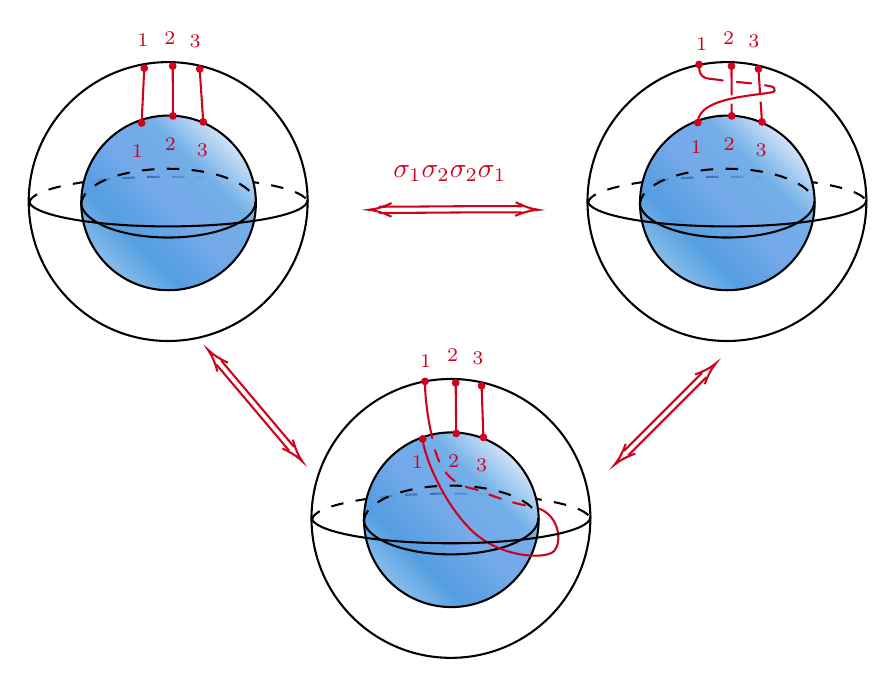
\begin{tikzpicture}[x=0.75pt,y=0.75pt,yscale=-1,xscale=1]
%uncomment if require: \path (0,310); %set diagram left start at 0, and has height of 310

%Shape: Arc [id:dp09992935330239217] 
\draw  [draw opacity=0][dash pattern={on 4.5pt off 4.5pt}] (128.51,85.86) .. controls (128.5,85.78) and (128.5,85.69) .. (128.5,85.6) .. controls (128.5,78.63) and (158.49,72.98) .. (195.49,72.98) .. controls (229.97,72.98) and (258.36,77.89) .. (262.08,84.2) -- (195.49,85.6) -- cycle ; \draw  [dash pattern={on 4.5pt off 4.5pt}] (128.51,85.86) .. controls (128.5,85.78) and (128.5,85.69) .. (128.5,85.6) .. controls (128.5,78.63) and (158.49,72.98) .. (195.49,72.98) .. controls (229.97,72.98) and (258.36,77.89) .. (262.08,84.2) ;  
%Shape: Ellipse [id:dp5022609554858339] 
\path  [shading=_nb0qb04h6,_3ktbl1rd2,path fading= _has4rknf2 ,fading transform={xshift=2}] (153.42,85.6) .. controls (153.42,62.37) and (172.25,43.53) .. (195.49,43.53) .. controls (218.73,43.53) and (237.57,62.37) .. (237.57,85.6) .. controls (237.57,108.84) and (218.73,127.68) .. (195.49,127.68) .. controls (172.25,127.68) and (153.42,108.84) .. (153.42,85.6) -- cycle ; % for fading 
 \draw   (153.42,85.6) .. controls (153.42,62.37) and (172.25,43.53) .. (195.49,43.53) .. controls (218.73,43.53) and (237.57,62.37) .. (237.57,85.6) .. controls (237.57,108.84) and (218.73,127.68) .. (195.49,127.68) .. controls (172.25,127.68) and (153.42,108.84) .. (153.42,85.6) -- cycle ; % for border 

%Shape: Ellipse [id:dp1138552774786783] 
\draw  [color={rgb, 255:red, 0; green, 0; blue, 0 }  ,draw opacity=1 ] (128.12,84.96) .. controls (128.12,47.85) and (158.2,17.77) .. (195.3,17.77) .. controls (232.41,17.77) and (262.49,47.85) .. (262.49,84.96) .. controls (262.49,122.06) and (232.41,152.14) .. (195.3,152.14) .. controls (158.2,152.14) and (128.12,122.06) .. (128.12,84.96) -- cycle ;
%Shape: Arc [id:dp2652675230393713] 
\draw  [draw opacity=0] (237.41,84.8) .. controls (237.41,84.85) and (237.41,84.9) .. (237.41,84.96) .. controls (237.41,94.53) and (218.56,102.29) .. (195.3,102.29) .. controls (172.78,102.29) and (154.38,95) .. (153.26,85.85) -- (195.3,84.96) -- cycle ; \draw   (237.41,84.8) .. controls (237.41,84.85) and (237.41,84.9) .. (237.41,84.96) .. controls (237.41,94.53) and (218.56,102.29) .. (195.3,102.29) .. controls (172.78,102.29) and (154.38,95) .. (153.26,85.85) ;  
%Shape: Arc [id:dp626190661691258] 
\draw  [draw opacity=0][dash pattern={on 4.5pt off 4.5pt}] (153.42,86.65) .. controls (153.42,86.6) and (153.42,86.55) .. (153.42,86.49) .. controls (153.42,76.92) and (172.27,69.16) .. (195.52,69.16) .. controls (218.05,69.16) and (236.44,76.44) .. (237.57,85.6) -- (195.52,86.49) -- cycle ; \draw  [dash pattern={on 4.5pt off 4.5pt}] (153.42,86.65) .. controls (153.42,86.6) and (153.42,86.55) .. (153.42,86.49) .. controls (153.42,76.92) and (172.27,69.16) .. (195.52,69.16) .. controls (218.05,69.16) and (236.44,76.44) .. (237.57,85.6) ;  
%Shape: Arc [id:dp2712356628787216] 
\draw  [draw opacity=0] (262.47,84.05) .. controls (262.48,84.14) and (262.49,84.22) .. (262.49,84.31) .. controls (262.49,91.28) and (232.4,96.93) .. (195.28,96.93) .. controls (160.71,96.93) and (132.23,92.03) .. (128.5,85.72) -- (195.28,84.31) -- cycle ; \draw   (262.47,84.05) .. controls (262.48,84.14) and (262.49,84.22) .. (262.49,84.31) .. controls (262.49,91.28) and (232.4,96.93) .. (195.28,96.93) .. controls (160.71,96.93) and (132.23,92.03) .. (128.5,85.72) ;  
%Curve Lines [id:da2789416130532578] 
\draw [color={rgb, 255:red, 208; green, 2; blue, 27 }  ,draw opacity=1 ]   (300.22,87.44) .. controls (295.44,87.44) and (296.78,87.44) .. (298.15,87.44) .. controls (306.06,87.44) and (315.12,87.37) .. (324.36,87.29) .. controls (326,87.28) and (327.64,87.27) .. (329.28,87.26) .. controls (336.91,87.2) and (344.55,87.15) .. (351.64,87.15) .. controls (359.22,87.15) and (366.17,87.21) .. (365.93,87.24)(300.21,90.44) .. controls (295.43,90.44) and (296.77,90.44) .. (298.15,90.44) .. controls (306.07,90.44) and (315.14,90.37) .. (324.39,90.29) .. controls (326.02,90.28) and (327.66,90.27) .. (329.3,90.26) .. controls (336.93,90.2) and (344.56,90.15) .. (351.64,90.15) .. controls (359.19,90.15) and (366.11,90.21) .. (365.77,90.24) ;
\draw [shift={(373.57,88.92)}, rotate = 181.94] [color={rgb, 255:red, 208; green, 2; blue, 27 }  ,draw opacity=1 ][line width=0.75]    (10.93,-3.29) .. controls (6.95,-1.4) and (3.31,-0.3) .. (0,0) .. controls (3.31,0.3) and (6.95,1.4) .. (10.93,3.29)   ;
\draw [shift={(291.99,88.92)}, rotate = 0.35] [color={rgb, 255:red, 208; green, 2; blue, 27 }  ,draw opacity=1 ][line width=0.75]    (10.93,-3.29) .. controls (6.95,-1.4) and (3.31,-0.3) .. (0,0) .. controls (3.31,0.3) and (6.95,1.4) .. (10.93,3.29)   ;

%Shape: Arc [id:dp9806762711371362] 
\draw  [draw opacity=0][dash pattern={on 4.5pt off 4.5pt}] (397.72,85.86) .. controls (397.71,85.78) and (397.71,85.69) .. (397.71,85.6) .. controls (397.71,78.63) and (427.7,72.98) .. (464.71,72.98) .. controls (499.18,72.98) and (527.58,77.89) .. (531.29,84.2) -- (464.71,85.6) -- cycle ; \draw  [dash pattern={on 4.5pt off 4.5pt}] (397.72,85.86) .. controls (397.71,85.78) and (397.71,85.69) .. (397.71,85.6) .. controls (397.71,78.63) and (427.7,72.98) .. (464.71,72.98) .. controls (499.18,72.98) and (527.58,77.89) .. (531.29,84.2) ;  
%Shape: Ellipse [id:dp7715704526733906] 
\path  [shading=_cjw6mg0w8,_ygtebnsje,path fading= _nnlfu2l9g ,fading transform={xshift=2}] (422.63,85.6) .. controls (422.63,62.37) and (441.47,43.53) .. (464.71,43.53) .. controls (487.94,43.53) and (506.78,62.37) .. (506.78,85.6) .. controls (506.78,108.84) and (487.94,127.68) .. (464.71,127.68) .. controls (441.47,127.68) and (422.63,108.84) .. (422.63,85.6) -- cycle ; % for fading 
 \draw   (422.63,85.6) .. controls (422.63,62.37) and (441.47,43.53) .. (464.71,43.53) .. controls (487.94,43.53) and (506.78,62.37) .. (506.78,85.6) .. controls (506.78,108.84) and (487.94,127.68) .. (464.71,127.68) .. controls (441.47,127.68) and (422.63,108.84) .. (422.63,85.6) -- cycle ; % for border 

%Shape: Ellipse [id:dp6012980525384373] 
\draw  [color={rgb, 255:red, 0; green, 0; blue, 0 }  ,draw opacity=1 ] (397.34,84.96) .. controls (397.34,47.85) and (427.41,17.77) .. (464.52,17.77) .. controls (501.62,17.77) and (531.7,47.85) .. (531.7,84.96) .. controls (531.7,122.06) and (501.62,152.14) .. (464.52,152.14) .. controls (427.41,152.14) and (397.34,122.06) .. (397.34,84.96) -- cycle ;
%Shape: Arc [id:dp5355877678219287] 
\draw  [draw opacity=0] (506.62,84.8) .. controls (506.62,84.85) and (506.62,84.9) .. (506.62,84.96) .. controls (506.62,94.53) and (487.77,102.29) .. (464.52,102.29) .. controls (441.99,102.29) and (423.59,95) .. (422.47,85.85) -- (464.52,84.96) -- cycle ; \draw   (506.62,84.8) .. controls (506.62,84.85) and (506.62,84.9) .. (506.62,84.96) .. controls (506.62,94.53) and (487.77,102.29) .. (464.52,102.29) .. controls (441.99,102.29) and (423.59,95) .. (422.47,85.85) ;  
%Shape: Arc [id:dp37890892566571455] 
\draw  [draw opacity=0][dash pattern={on 4.5pt off 4.5pt}] (422.63,86.65) .. controls (422.63,86.6) and (422.63,86.55) .. (422.63,86.49) .. controls (422.63,76.92) and (441.48,69.16) .. (464.73,69.16) .. controls (487.26,69.16) and (505.66,76.44) .. (506.78,85.6) -- (464.73,86.49) -- cycle ; \draw  [dash pattern={on 4.5pt off 4.5pt}] (422.63,86.65) .. controls (422.63,86.6) and (422.63,86.55) .. (422.63,86.49) .. controls (422.63,76.92) and (441.48,69.16) .. (464.73,69.16) .. controls (487.26,69.16) and (505.66,76.44) .. (506.78,85.6) ;  
%Shape: Arc [id:dp1519720326100238] 
\draw  [draw opacity=0] (531.69,84.05) .. controls (531.7,84.14) and (531.7,84.22) .. (531.7,84.31) .. controls (531.7,91.28) and (501.61,96.93) .. (464.5,96.93) .. controls (429.92,96.93) and (401.45,92.03) .. (397.71,85.72) -- (464.5,84.31) -- cycle ; \draw   (531.69,84.05) .. controls (531.7,84.14) and (531.7,84.22) .. (531.7,84.31) .. controls (531.7,91.28) and (501.61,96.93) .. (464.5,96.93) .. controls (429.92,96.93) and (401.45,92.03) .. (397.71,85.72) ;  
%Curve Lines [id:da9865463652711379] 
\draw [color={rgb, 255:red, 208; green, 2; blue, 27 }  ,draw opacity=1 ][line width=0.75] [line join = round][line cap = round]   (450.49,46.92) .. controls (450.49,32.93) and (487.49,33.92) .. (487.49,31.59) .. controls (487.49,29.25) and (486.08,29.62) .. (482.82,28.92) ;
\draw [shift={(450.49,46.92)}, rotate = 270] [color={rgb, 255:red, 208; green, 2; blue, 27 }  ,draw opacity=1 ][fill={rgb, 255:red, 208; green, 2; blue, 27 }  ,fill opacity=1 ][line width=0.75] [line join = round][line cap = round]     (0, 0) circle [x radius= 1.34, y radius= 1.34]   ;
%Curve Lines [id:da4910039491295255] 
\draw [color={rgb, 255:red, 208; green, 2; blue, 27 }  ,draw opacity=1 ][line width=0.75] [line join = round][line cap = round]   (476.25,28.02) .. controls (473.91,27.79) and (471.58,27.56) .. (469.25,27.33) ;
%Curve Lines [id:da500237227046332] 
\draw [color={rgb, 255:red, 208; green, 2; blue, 27 }  ,draw opacity=1 ][line width=0.75] [line join = round][line cap = round]   (462.49,26.63) .. controls (455.03,25.23) and (451.07,27.03) .. (451.07,18.93) ;
\draw [shift={(451.07,18.93)}, rotate = 270] [color={rgb, 255:red, 208; green, 2; blue, 27 }  ,draw opacity=1 ][fill={rgb, 255:red, 208; green, 2; blue, 27 }  ,fill opacity=1 ][line width=0.75] [line join = round][line cap = round]     (0, 0) circle [x radius= 1.34, y radius= 1.34]   ;
%Shape: Arc [id:dp04669225929070464] 
\draw  [draw opacity=0][dash pattern={on 4.5pt off 4.5pt}] (264.75,238.52) .. controls (264.74,238.43) and (264.73,238.35) .. (264.73,238.26) .. controls (264.73,231.29) and (294.73,225.64) .. (331.73,225.64) .. controls (366.21,225.64) and (394.6,230.54) .. (398.31,236.85) -- (331.73,238.26) -- cycle ; \draw  [dash pattern={on 4.5pt off 4.5pt}] (264.75,238.52) .. controls (264.74,238.43) and (264.73,238.35) .. (264.73,238.26) .. controls (264.73,231.29) and (294.73,225.64) .. (331.73,225.64) .. controls (366.21,225.64) and (394.6,230.54) .. (398.31,236.85) ;  
%Shape: Ellipse [id:dp9291040830872814] 
\path  [shading=_qirw9k7hq,_imklbjwpz,path fading= _oc1vcgmvg ,fading transform={xshift=2}] (289.66,238.26) .. controls (289.66,215.02) and (308.49,196.18) .. (331.73,196.18) .. controls (354.97,196.18) and (373.81,215.02) .. (373.81,238.26) .. controls (373.81,261.5) and (354.97,280.33) .. (331.73,280.33) .. controls (308.49,280.33) and (289.66,261.5) .. (289.66,238.26) -- cycle ; % for fading 
 \draw   (289.66,238.26) .. controls (289.66,215.02) and (308.49,196.18) .. (331.73,196.18) .. controls (354.97,196.18) and (373.81,215.02) .. (373.81,238.26) .. controls (373.81,261.5) and (354.97,280.33) .. (331.73,280.33) .. controls (308.49,280.33) and (289.66,261.5) .. (289.66,238.26) -- cycle ; % for border 

%Shape: Ellipse [id:dp5148861882664881] 
\draw  [color={rgb, 255:red, 0; green, 0; blue, 0 }  ,draw opacity=1 ] (264.36,237.61) .. controls (264.36,200.51) and (294.44,170.43) .. (331.54,170.43) .. controls (368.65,170.43) and (398.73,200.51) .. (398.73,237.61) .. controls (398.73,274.72) and (368.65,304.8) .. (331.54,304.8) .. controls (294.44,304.8) and (264.36,274.72) .. (264.36,237.61) -- cycle ;
%Shape: Arc [id:dp7396011144157884] 
\draw  [draw opacity=0] (373.64,237.45) .. controls (373.65,237.51) and (373.65,237.56) .. (373.65,237.61) .. controls (373.65,247.18) and (354.8,254.94) .. (331.54,254.94) .. controls (309.01,254.94) and (290.62,247.66) .. (289.49,238.5) -- (331.54,237.61) -- cycle ; \draw   (373.64,237.45) .. controls (373.65,237.51) and (373.65,237.56) .. (373.65,237.61) .. controls (373.65,247.18) and (354.8,254.94) .. (331.54,254.94) .. controls (309.01,254.94) and (290.62,247.66) .. (289.49,238.5) ;  
%Shape: Arc [id:dp757316946645815] 
\draw  [draw opacity=0][dash pattern={on 4.5pt off 4.5pt}] (289.66,239.31) .. controls (289.65,239.26) and (289.65,239.2) .. (289.65,239.15) .. controls (289.65,229.58) and (308.5,221.82) .. (331.76,221.82) .. controls (354.29,221.82) and (372.68,229.1) .. (373.81,238.26) -- (331.76,239.15) -- cycle ; \draw  [dash pattern={on 4.5pt off 4.5pt}] (289.66,239.31) .. controls (289.65,239.26) and (289.65,239.2) .. (289.65,239.15) .. controls (289.65,229.58) and (308.5,221.82) .. (331.76,221.82) .. controls (354.29,221.82) and (372.68,229.1) .. (373.81,238.26) ;  
%Curve Lines [id:da5498171971577632] 
\draw [color={rgb, 255:red, 208; green, 2; blue, 27 }  ,draw opacity=1 ][line width=0.75] [line join = round][line cap = round]   (317.91,199.33) .. controls (318.73,207.49) and (327.18,229.1) .. (341.05,242.96) .. controls (354.92,256.83) and (377.76,257.65) .. (381.43,253.16) .. controls (385.1,248.67) and (383.63,236.66) .. (374.25,232.99) ;
\draw [shift={(317.91,199.33)}, rotate = 84.29] [color={rgb, 255:red, 208; green, 2; blue, 27 }  ,draw opacity=1 ][fill={rgb, 255:red, 208; green, 2; blue, 27 }  ,fill opacity=1 ][line width=0.75] [line join = round][line cap = round]     (0, 0) circle [x radius= 1.34, y radius= 1.34]   ;
%Curve Lines [id:da2758655601652622] 
\draw [color={rgb, 255:red, 208; green, 2; blue, 27 }  ,draw opacity=1 ][line width=0.75] [line join = round][line cap = round] [dash pattern={on 4.5pt off 4.5pt}]  (367.25,231.32) .. controls (359.67,229.77) and (350.07,226.36) .. (345.58,224.32) .. controls (341.09,222.28) and (326.58,223.65) .. (322.29,197.69) ;
%Curve Lines [id:da14444386151047484] 
\draw [color={rgb, 255:red, 208; green, 2; blue, 27 }  ,draw opacity=1 ][line width=0.75] [line join = round][line cap = round]   (322.29,197.69) .. controls (320.58,190.32) and (319.02,179.74) .. (319.02,171.58) ;
\draw [shift={(319.02,171.58)}, rotate = 270] [color={rgb, 255:red, 208; green, 2; blue, 27 }  ,draw opacity=1 ][fill={rgb, 255:red, 208; green, 2; blue, 27 }  ,fill opacity=1 ][line width=0.75] [line join = round][line cap = round]     (0, 0) circle [x radius= 1.34, y radius= 1.34]   ;
%Shape: Arc [id:dp6413900583710832] 
\draw  [draw opacity=0] (398.71,236.71) .. controls (398.72,236.79) and (398.73,236.88) .. (398.73,236.97) .. controls (398.73,243.94) and (368.64,249.59) .. (331.52,249.59) .. controls (296.95,249.59) and (268.47,244.68) .. (264.74,238.38) -- (331.52,236.97) -- cycle ; \draw   (398.71,236.71) .. controls (398.72,236.79) and (398.73,236.88) .. (398.73,236.97) .. controls (398.73,243.94) and (368.64,249.59) .. (331.52,249.59) .. controls (296.95,249.59) and (268.47,244.68) .. (264.74,238.38) ;  
%Straight Lines [id:da6629690084069055] 
\draw [color={rgb, 255:red, 208; green, 2; blue, 27 }  ,draw opacity=1 ]   (454.63,169.59) -- (417.05,207.18)(452.51,167.47) -- (414.92,205.06) ;
\draw [shift={(410.33,211.78)}, rotate = 315] [color={rgb, 255:red, 208; green, 2; blue, 27 }  ,draw opacity=1 ][line width=0.75]    (10.93,-3.29) .. controls (6.95,-1.4) and (3.31,-0.3) .. (0,0) .. controls (3.31,0.3) and (6.95,1.4) .. (10.93,3.29)   ;
\draw [shift={(459.23,162.87)}, rotate = 135] [color={rgb, 255:red, 208; green, 2; blue, 27 }  ,draw opacity=1 ][line width=0.75]    (10.93,-3.29) .. controls (6.95,-1.4) and (3.31,-0.3) .. (0,0) .. controls (3.31,0.3) and (6.95,1.4) .. (10.93,3.29)   ;
%Straight Lines [id:da8162131984506948] 
\draw [color={rgb, 255:red, 208; green, 2; blue, 27 }  ,draw opacity=1 ]   (220.8,161.49) -- (255.91,203.06)(218.51,163.43) -- (253.62,205) ;
\draw [shift={(259.93,210.14)}, rotate = 229.81] [color={rgb, 255:red, 208; green, 2; blue, 27 }  ,draw opacity=1 ][line width=0.75]    (10.93,-3.29) .. controls (6.95,-1.4) and (3.31,-0.3) .. (0,0) .. controls (3.31,0.3) and (6.95,1.4) .. (10.93,3.29)   ;
\draw [shift={(214.49,156.35)}, rotate = 49.81] [color={rgb, 255:red, 208; green, 2; blue, 27 }  ,draw opacity=1 ][line width=0.75]    (10.93,-3.29) .. controls (6.95,-1.4) and (3.31,-0.3) .. (0,0) .. controls (3.31,0.3) and (6.95,1.4) .. (10.93,3.29)   ;

% Text Node
\draw (302.28,66.24) node [anchor=north west][inner sep=0.75pt]  [color={rgb, 255:red, 208; green, 2; blue, 27 }  ,opacity=1 ]  {$\sigma _{1} \sigma _{2} \sigma _{2} \sigma _{1}$};
% Text Node
\draw (178.96,2.66) node [anchor=north west][inner sep=0.75pt]  [font=\scriptsize,color={rgb, 255:red, 208; green, 2; blue, 27 }  ,opacity=1 ]  {$1$};
% Text Node
\draw (191.93,1.68) node [anchor=north west][inner sep=0.75pt]  [font=\scriptsize,color={rgb, 255:red, 208; green, 2; blue, 27 }  ,opacity=1 ]  {$2$};
% Text Node
\draw (204.09,3.07) node [anchor=north west][inner sep=0.75pt]  [font=\scriptsize,color={rgb, 255:red, 208; green, 2; blue, 27 }  ,opacity=1 ]  {$3$};
% Text Node
\draw (176.35,56.07) node [anchor=north west][inner sep=0.75pt]  [font=\scriptsize,color={rgb, 255:red, 208; green, 2; blue, 27 }  ,opacity=1 ]  {$1$};
% Text Node
\draw (192.18,52.68) node [anchor=north west][inner sep=0.75pt]  [font=\scriptsize,color={rgb, 255:red, 208; green, 2; blue, 27 }  ,opacity=1 ]  {$2$};
% Text Node
\draw (207.6,55.58) node [anchor=north west][inner sep=0.75pt]  [font=\scriptsize,color={rgb, 255:red, 208; green, 2; blue, 27 }  ,opacity=1 ]  {$3$};
% Text Node
\draw (448.18,4.66) node [anchor=north west][inner sep=0.75pt]  [font=\scriptsize,color={rgb, 255:red, 208; green, 2; blue, 27 }  ,opacity=1 ]  {$1$};
% Text Node
\draw (461.15,1.68) node [anchor=north west][inner sep=0.75pt]  [font=\scriptsize,color={rgb, 255:red, 208; green, 2; blue, 27 }  ,opacity=1 ]  {$2$};
% Text Node
\draw (473.3,3.07) node [anchor=north west][inner sep=0.75pt]  [font=\scriptsize,color={rgb, 255:red, 208; green, 2; blue, 27 }  ,opacity=1 ]  {$3$};
% Text Node
\draw (445.57,54.07) node [anchor=north west][inner sep=0.75pt]  [font=\scriptsize,color={rgb, 255:red, 208; green, 2; blue, 27 }  ,opacity=1 ]  {$1$};
% Text Node
\draw (461.39,52.68) node [anchor=north west][inner sep=0.75pt]  [font=\scriptsize,color={rgb, 255:red, 208; green, 2; blue, 27 }  ,opacity=1 ]  {$2$};
% Text Node
\draw (476.81,55.58) node [anchor=north west][inner sep=0.75pt]  [font=\scriptsize,color={rgb, 255:red, 208; green, 2; blue, 27 }  ,opacity=1 ]  {$3$};
% Text Node
\draw (315.2,157.31) node [anchor=north west][inner sep=0.75pt]  [font=\scriptsize,color={rgb, 255:red, 208; green, 2; blue, 27 }  ,opacity=1 ]  {$1$};
% Text Node
\draw (328.17,154.33) node [anchor=north west][inner sep=0.75pt]  [font=\scriptsize,color={rgb, 255:red, 208; green, 2; blue, 27 }  ,opacity=1 ]  {$2$};
% Text Node
\draw (340.33,155.72) node [anchor=north west][inner sep=0.75pt]  [font=\scriptsize,color={rgb, 255:red, 208; green, 2; blue, 27 }  ,opacity=1 ]  {$3$};
% Text Node
\draw (311.26,206.06) node [anchor=north west][inner sep=0.75pt]  [font=\scriptsize,color={rgb, 255:red, 208; green, 2; blue, 27 }  ,opacity=1 ]  {$1$};
% Text Node
\draw (328.75,205.67) node [anchor=north west][inner sep=0.75pt]  [font=\scriptsize,color={rgb, 255:red, 208; green, 2; blue, 27 }  ,opacity=1 ]  {$2$};
% Text Node
\draw (342.17,207.57) node [anchor=north west][inner sep=0.75pt]  [font=\scriptsize,color={rgb, 255:red, 208; green, 2; blue, 27 }  ,opacity=1 ]  {$3$};
% Connection
\draw [color={rgb, 255:red, 208; green, 2; blue, 27 }  ,draw opacity=1 ]   (183.8,20.66) -- (182.51,47.07) ;
\draw [shift={(182.51,47.07)}, rotate = 92.8] [color={rgb, 255:red, 208; green, 2; blue, 27 }  ,draw opacity=1 ][fill={rgb, 255:red, 208; green, 2; blue, 27 }  ,fill opacity=1 ][line width=0.75]      (0, 0) circle [x radius= 1.34, y radius= 1.34]   ;
\draw [shift={(183.8,20.66)}, rotate = 92.8] [color={rgb, 255:red, 208; green, 2; blue, 27 }  ,draw opacity=1 ][fill={rgb, 255:red, 208; green, 2; blue, 27 }  ,fill opacity=1 ][line width=0.75]      (0, 0) circle [x radius= 1.34, y radius= 1.34]   ;
% Connection
\draw [color={rgb, 255:red, 208; green, 2; blue, 27 }  ,draw opacity=1 ]   (197.5,19.68) -- (197.61,43.68) ;
\draw [shift={(197.61,43.68)}, rotate = 89.73] [color={rgb, 255:red, 208; green, 2; blue, 27 }  ,draw opacity=1 ][fill={rgb, 255:red, 208; green, 2; blue, 27 }  ,fill opacity=1 ][line width=0.75]      (0, 0) circle [x radius= 1.34, y radius= 1.34]   ;
\draw [shift={(197.5,19.68)}, rotate = 89.73] [color={rgb, 255:red, 208; green, 2; blue, 27 }  ,draw opacity=1 ][fill={rgb, 255:red, 208; green, 2; blue, 27 }  ,fill opacity=1 ][line width=0.75]      (0, 0) circle [x radius= 1.34, y radius= 1.34]   ;
% Connection
\draw [color={rgb, 255:red, 208; green, 2; blue, 27 }  ,draw opacity=1 ]   (210.49,21.07) -- (212.2,46.58) ;
\draw [shift={(212.2,46.58)}, rotate = 86.18] [color={rgb, 255:red, 208; green, 2; blue, 27 }  ,draw opacity=1 ][fill={rgb, 255:red, 208; green, 2; blue, 27 }  ,fill opacity=1 ][line width=0.75]      (0, 0) circle [x radius= 1.34, y radius= 1.34]   ;
\draw [shift={(210.49,21.07)}, rotate = 86.18] [color={rgb, 255:red, 208; green, 2; blue, 27 }  ,draw opacity=1 ][fill={rgb, 255:red, 208; green, 2; blue, 27 }  ,fill opacity=1 ][line width=0.75]      (0, 0) circle [x radius= 1.34, y radius= 1.34]   ;
% Connection
\draw [color={rgb, 255:red, 208; green, 2; blue, 27 }  ,draw opacity=1 ]   (479.7,21.07) -- (480.49,32.85)(480.76,36.84) -- (481.41,46.58) ;
\draw [shift={(481.41,46.58)}, rotate = 86.18] [color={rgb, 255:red, 208; green, 2; blue, 27 }  ,draw opacity=1 ][fill={rgb, 255:red, 208; green, 2; blue, 27 }  ,fill opacity=1 ][line width=0.75]      (0, 0) circle [x radius= 1.34, y radius= 1.34]   ;
\draw [shift={(479.7,21.07)}, rotate = 86.18] [color={rgb, 255:red, 208; green, 2; blue, 27 }  ,draw opacity=1 ][fill={rgb, 255:red, 208; green, 2; blue, 27 }  ,fill opacity=1 ][line width=0.75]      (0, 0) circle [x radius= 1.34, y radius= 1.34]   ;
% Connection
\draw [color={rgb, 255:red, 208; green, 2; blue, 27 }  ,draw opacity=1 ]   (466.71,19.68) -- (466.78,33.76)(466.8,37.76) -- (466.83,43.68) ;
\draw [shift={(466.83,43.68)}, rotate = 89.73] [color={rgb, 255:red, 208; green, 2; blue, 27 }  ,draw opacity=1 ][fill={rgb, 255:red, 208; green, 2; blue, 27 }  ,fill opacity=1 ][line width=0.75]      (0, 0) circle [x radius= 1.34, y radius= 1.34]   ;
\draw [shift={(466.71,19.68)}, rotate = 89.73] [color={rgb, 255:red, 208; green, 2; blue, 27 }  ,draw opacity=1 ][fill={rgb, 255:red, 208; green, 2; blue, 27 }  ,fill opacity=1 ][line width=0.75]      (0, 0) circle [x radius= 1.34, y radius= 1.34]   ;
% Connection
\draw [color={rgb, 255:red, 208; green, 2; blue, 27 }  ,draw opacity=1 ]   (346.31,173.72) -- (347.19,198.57) ;
\draw [shift={(347.19,198.57)}, rotate = 87.97] [color={rgb, 255:red, 208; green, 2; blue, 27 }  ,draw opacity=1 ][fill={rgb, 255:red, 208; green, 2; blue, 27 }  ,fill opacity=1 ][line width=0.75]      (0, 0) circle [x radius= 1.34, y radius= 1.34]   ;
\draw [shift={(346.31,173.72)}, rotate = 87.97] [color={rgb, 255:red, 208; green, 2; blue, 27 }  ,draw opacity=1 ][fill={rgb, 255:red, 208; green, 2; blue, 27 }  ,fill opacity=1 ][line width=0.75]      (0, 0) circle [x radius= 1.34, y radius= 1.34]   ;
% Connection
\draw [color={rgb, 255:red, 208; green, 2; blue, 27 }  ,draw opacity=1 ]   (333.82,172.33) -- (334.1,196.67) ;
\draw [shift={(334.1,196.67)}, rotate = 89.35] [color={rgb, 255:red, 208; green, 2; blue, 27 }  ,draw opacity=1 ][fill={rgb, 255:red, 208; green, 2; blue, 27 }  ,fill opacity=1 ][line width=0.75]      (0, 0) circle [x radius= 1.34, y radius= 1.34]   ;
\draw [shift={(333.82,172.33)}, rotate = 89.35] [color={rgb, 255:red, 208; green, 2; blue, 27 }  ,draw opacity=1 ][fill={rgb, 255:red, 208; green, 2; blue, 27 }  ,fill opacity=1 ][line width=0.75]      (0, 0) circle [x radius= 1.34, y radius= 1.34]   ;
\end{tikzpicture}
\caption{Effect of  $\sigma _{1} \sigma _{2} \sigma _{2} \sigma _{1}$.}
\label{fig:s1s2s2s1}
\end{figure}
This means the line can get cross the sphere and return to trivial configuration.

\section{About the Symmetric Group}
Show that \eqref{eq:definingRelationsOfBraidGroup} also hold for the generators of the symmetric group $S_{M}$ on $M$ particles, where $\sigma _{i}$ exchanges particle $i$ and $i+1$. In the symmetric group we have the additional condition that $\sigma _{i}^{2} =1$. Prove the statement used in section 3.4.1 that there are only two one-dimensional representations of the symmetric group. Hint: The proof is just a few lines. Use $\rho ( \sigma _{i}) \rho ( \sigma _{j}) =\rho ( \sigma _{i} \sigma _{j})$ where $\rho $ is a representation.

\paragraph{Answer}
(a) For the element in symmetric group $S_{M}$, we can write $\sigma _{i}$ as $( i,i+1)$. Then
\begin{equation*}
\sigma _{i} \sigma _{j} =( i,i+1)( j,j+1) =( j,j+1)( i,i+1) =\sigma _{j} \sigma _{i} ,\quad |i-j| >1,
\end{equation*}
is trivial. The first one gives:
\begin{equation*}
\begin{aligned}
\sigma _{i} \sigma _{i+1} \sigma _{i} & =( i,i+1)( i+1,i+2)( i,i+1)\\
 & =( i,i+1,i+2)( i,i+1)\\
 & =( i+2,i,i+1)( i,i+1)\\
 & =( i+2,i)
\end{aligned}
\end{equation*}
while
\begin{equation*}
\begin{aligned}
\sigma _{i+1} \sigma _{i} \sigma _{i+1} & =( i+1,i+2)( i,i+1)( i+1,i+2)\\
 & =( i+2,i+1,i)( i+1,i+2)\\
 & =( i,i+2,i+1)( i+1,i+2)\\
 & =( i,i+2) =\sigma _{i} \sigma _{i+1} \sigma _{i} ,
\end{aligned}
\end{equation*}
which also holds.

(b) Suppose $\rho ( \sigma _{1}) =c$, which means
\begin{equation*}
\rho ( \sigma _{1}) \rho ( \sigma _{1}) =c^{2} =\rho ( \sigma _{1} \sigma _{1}) =\rho ( I) =1,
\end{equation*}
thus $c^{2} =1$ have only two possibilities $c=\pm 1$. Suppose there exist $i$, such that $\rho ( \sigma _{i}) =1$ while $\rho ( \sigma _{i+1}) =-1$, then according to \eqref{eq:definingRelationsOfBraidGroup}:
\begin{equation*}
\rho ( \sigma _{i} \sigma _{i+1} \sigma _{i}) =-1\neq 1=\rho ( \sigma _{i} \sigma _{i+1} \sigma _{i}) .
\end{equation*}
So $\rho ( \sigma _{i})$ and $\rho ( \sigma _{i+1})$ have the same sign, either $1$ or $-1$, then all $\rho ( \sigma _{i})$ have the same sign. We also know any permutation can be generate by $\sigma _{i} ,i\in \{1,\cdots ,M\}$, we can see there are only two kinds of 1-d representation of $S_{M}$. 

\section{Ising Anyons and Majorana Fermions}
The most commonly discussed type of nonabelian anyon is the Ising anyon (we will discuss this in more depth later). Ising anyons occurs in the Moore-Read quantum Hall state $(\nu =5/2)$, as well as in any chiral $p$-wave superconductor and in recently experimentally relevant so called "Majorana" systems.

The nonabelian statistics of these anyons may be described in terms of Majorana fermions by attaching a Majorana operator to each anyon. The Hamiltonian for these Majoranas is zero - they are completely noninteracting. In case you haven't seen them before, Majorana Fermions $\gamma _{j}$ satisfy the anticommutation relation
\begin{equation*}
\{\gamma _{i} ,\gamma _{j}\} \equiv \gamma _{i} \gamma _{j} +\gamma _{j} \gamma _{i} =2\delta _{ij}
\end{equation*}
as well as being self conjugate $\gamma _{i}^{\dagger } =\gamma _{i}$.
\begin{enumerate}
\item Show that the ground state degeneracy of a system with $2N$ Majoranas is $2^{N}$ if the Hamiltonian is zero. Thus conclude that each \textit{pair} of Ising anyons is a two-state system. Hint: Construct a regular (Dirac) fermion operator from two Majorana fermion operators. For example,\begin{equation*}
c^{\dagger } =\frac{1}{2}( \gamma _{1} +\mathrm{i} \gamma _{2})
\end{equation*}will then satisfy the usual fermion anti-commutation $\{c,c^{\dagger } \}=cc^{\dagger } +c^{\dagger } c=\mathds{1}$. (If you haven't run into fermion creation operators yet, you might want to read up on this first!) There is more discussion of this transformation in later exercises $9.7$ and $10.2$.
\item When anyon $i$ is exchanged clockwise with anyon $j$, the unitary transformation that occurs on the ground state is\begin{equation}
U_{ij} =\frac{\mathrm{e}^{\mathrm{i} \alpha }}{\sqrt{2}}[ 1+\gamma _{i} \gamma _{j}] ,i< j.
\label{eq:representationOfBraidGroup}
\end{equation}for some real value of $\alpha $. Show that these unitary operators form a representation of the braid group. (Refer back to the previous problem, "About the Braid Group"). In other words we must show that replacing $\sigma _{i}$ with $U_{i,i+1}$ in \eqref{eq:definingRelationsOfBraidGroup} yields equalities. This representation is $2^{N}$ dimensional since the ground state degeneracy is $2^{N}$.
\item Consider the operator\begin{equation*}
\gamma ^{\mathrm{FIVE}} =(\mathrm{i} )^{N} \gamma _{1} \gamma _{2} \dotsc \gamma _{2N}
\end{equation*}(the notation five is in analogy with the $\gamma ^{5}$ of the Dirac gamma matrices). Show that the eigenvalues of $\gamma ^{\text{FIVE }}$ are $\pm 1$. Further show that this eigenvalue remains unchanged under any braid operation. Conclude that we actually have two $2^{N-1}$ dimensional representations of the braid group. We will assume that any particular system of Ising anyons is in one of these two representations.
\item Thus, 4 Ising anyons on a sphere comprise a single 2-state system, or a qubit. Show that by only braiding these four Ising anyons one cannot obtain all possible unitary operation on this qubit. Indeed, braiding Ising anyons is not sufficient to build a quantum computer. [Part (d) is not required to solve parts (e) and (f)]
\item (bit harder)Now consider $2N$ Ising anyons on a sphere (See above problem "About the braid group" for information about the braid group on a sphere). Show that in order for either one of the $2^{N-1}$ dimensional representations of the braid group to satisfy the sphere relation, \eqref{eq:definingRelationOfBraidGroupOnSphere}, one must choose the right abelian phase $\alpha $ in \eqref{eq:representationOfBraidGroup}. Determine this phase.
\item (a bit harder) The value you just determined is not quite right. It should look a bit unnatural as the abelian phase associated with a braid depends on the number of anyons in the system. Go back to \eqref{eq:definingRelationOfBraidGroupOnSphere} and insert an additional abelian phase on the right hand side which will make the final result of part (e) independent of the number of anyons in the system. In fact, there should be such an additional factor - to figure out where it comes from, go back and look again at the geometric "proof" of \eqref{eq:definingRelationOfBraidGroupOnSphere}. Note that the proof involves a self-twist of one of the anyon world lines. The additional phase you added is associated with one particle twisting around itself. The relation between self-rotation of a single particle and exchange of two particles is a generalized spin-statistics theorem.
\end{enumerate}

\paragraph{Answer}
We can use two Majorana fermions to construct a normal Dirac fermion by the transformation
\begin{equation*}
c_{i}^{\dagger } =\frac{1}{2}( \gamma _{2i-1} +\mathrm{i} \gamma _{2i}) ,\quad c_{i} =\frac{1}{2}( \gamma _{2i-1} -\mathrm{i} \gamma _{2i}) ,
\end{equation*}
where $i=1,\cdots ,N$. We can check:
\begin{equation*}
\begin{aligned}
\{c_{i} ,c_{j}^{\dagger } \} & =c_{i} c_{j}^{\dagger } +c_{j}^{\dagger } c_{i} =\frac{1}{4}( \gamma _{2i-1} -\mathrm{i} \gamma _{2i})( \gamma _{2j-1} +\mathrm{i} \gamma _{2j}) +\frac{1}{4}( \gamma _{2j-1} +\mathrm{i} \gamma _{2j})( \gamma _{2i-1} -\mathrm{i} \gamma _{2i})\\
 & =\frac{1}{4}( \gamma _{2i-1} \gamma _{2j-1} -\mathrm{i} \gamma _{2i} \gamma _{2j-1} +\mathrm{i} \gamma _{2i-1} \gamma _{2j} +\gamma _{2i} \gamma _{2j} +( i\leftrightarrow j,\mathrm{i} \leftrightarrow -\mathrm{i}))\\
 & =\delta _{ij} .
\end{aligned}
\end{equation*}
Therefore, the fermion number operator is given by $\sum _{i=1}^{N} n_{i} =\sum _{i=1}^{N} c_{i}^{\dagger } c_{i} =\sum _{i}^{N}( 1+\mathrm{i} \gamma _{2i} \gamma _{2i-1}) /2$. Obviously it is a projection operator $n_{i}^{2} =n_{i}$ so it only has eigenvalue 1 or 0, i.e. the occupied and empty state. Therefore, the ground state of the system has the degeneracy of $2^{N}$ because there are $N$ fermions. 



(b) We just need to show the map $\sigma _{i} \mapsto U_{i,i+1}$ induce an isomorphism. Here we prove the second equality first:
\begin{equation*}
\begin{aligned}
\sigma _{i} \sigma _{j} & \mapsto U_{i,i+1} U_{j,j+1}\\
 & =\frac{\mathrm{e}^{2\mathrm{i} \alpha }}{2}( 1+\gamma _{i} \gamma _{i+1})( 1+\gamma _{j} \gamma _{j+1})\\
 & =\frac{\mathrm{e}^{2\mathrm{i} \alpha }}{2}( 1+\gamma _{j} \gamma _{j+1} +\gamma _{i} \gamma _{i+1} +\gamma _{i} \gamma _{i+1} \gamma _{j} \gamma _{j+1}) .
\end{aligned}
\end{equation*}
While for
\begin{equation*}
\begin{aligned}
\sigma _{j} \sigma _{i} & \mapsto U_{j,j+1} U_{i,i+1}\\
 & =\frac{\mathrm{e}^{2\mathrm{i} \alpha }}{2}( 1+\gamma _{j} \gamma _{j+1})( 1+\gamma _{i} \gamma _{i+1})\\
 & =\frac{\mathrm{e}^{2\mathrm{i} \alpha }}{2}( 1+\gamma _{i} \gamma _{i+1} +\gamma _{j} \gamma _{j+1} +\gamma _{j} \gamma _{j+1} \gamma _{i} \gamma _{i+1}) .
\end{aligned}
\end{equation*}
According to the anti-commutation relation:
\begin{equation*}
\{\gamma _{i} ,\gamma _{j}\} =2\delta _{ij} =0=\gamma _{i} \gamma _{j} +\gamma _{j} \gamma _{i} \Rightarrow \gamma _{i} \gamma _{j} =-\gamma _{j} \gamma _{i} ,
\end{equation*}
So $\gamma _{j} \gamma _{j+1} \gamma _{i} \gamma _{i+1} =-\gamma _{j} \gamma _{i} \gamma _{j+1} \gamma _{i+1} =\gamma _{i} \gamma _{j} \gamma _{j+1} \gamma _{i+1} =-\gamma _{i} \gamma _{j} \gamma _{i+1} \gamma _{j+1} =\gamma _{i} \gamma _{i+1} \gamma _{j} \gamma _{j+1}$. Therefore we have
\begin{equation*}
U_{i,i+1} U_{j,j+1} =U_{j,j+1} U_{i,i+1} .
\end{equation*}
For the first identity:
\begin{equation*}
\begin{aligned}
\sigma _{i} \sigma _{i+1} \sigma _{i} & \mapsto U_{i,i+1} U_{i+1,i+2} U_{i,i+1}\\
 & =\frac{\mathrm{e}^{3\mathrm{i} \alpha }}{2\sqrt{2}}( 1+\gamma _{i} \gamma _{i+1})( 1+\gamma _{i+1} \gamma _{i+2})( 1+\gamma _{i} \gamma _{i+1})\\
 & =\frac{\mathrm{e}^{3\mathrm{i} \alpha }}{2\sqrt{2}}( 1+\gamma _{i} \gamma _{i+1} +\gamma _{i+1} \gamma _{i+2} +\gamma _{i} \gamma _{i+1} \gamma _{i+1} \gamma _{i+2})( 1+\gamma _{i} \gamma _{i+1}) .
\end{aligned}
\end{equation*}
According to the anti-commutation relation:
\begin{equation*}
\{\gamma _{i} ,\gamma _{i}\} =2\delta _{ii} =2=2\gamma _{i} \gamma _{i} ,
\end{equation*}
So
\begin{equation*}
\begin{aligned}
\sigma _{i} \sigma _{i+1} \sigma _{i} \mapsto  & \frac{\mathrm{e}^{3\mathrm{i} \alpha }}{2\sqrt{2}}( 1+\gamma _{i} \gamma _{i+1} +\gamma _{i+1} \gamma _{i+2} +\gamma _{i} \gamma _{i+2})( 1+\gamma _{i} \gamma _{i+1})\\
 & =\frac{\mathrm{e}^{3\mathrm{i} \alpha }}{\sqrt{2}}( \gamma _{i} \gamma _{i+1} +\gamma _{i+1} \gamma _{i+2}) .
\end{aligned}
\end{equation*}
For the second half:
\begin{equation*}
\begin{aligned}
\sigma _{i+1} \sigma _{i} \sigma _{i+1} & \mapsto U_{i+1,i+2} U_{i,i+1} U_{i+1,i+2}\\
 & =\frac{\mathrm{e}^{3\mathrm{i} \alpha }}{2\sqrt{2}}( 1+\gamma _{i+1} \gamma _{i+2})( 1+\gamma _{i} \gamma _{i+1})( 1+\gamma _{i+1} \gamma _{i+2})\\
 & =\frac{\mathrm{e}^{3\mathrm{i} \alpha }}{2\sqrt{2}}( 1+\gamma _{i} \gamma _{i+1} +\gamma _{i+1} \gamma _{i+2} +\gamma _{i+2} \gamma _{i})( 1+\gamma _{i+1} \gamma _{i+2})\\
 & =\frac{\mathrm{e}^{3\mathrm{i} \alpha }}{\sqrt{2}}( \gamma _{i} \gamma _{i+1} +\gamma _{i+1} \gamma _{i+2}) .
\end{aligned}
\end{equation*}
So we have checked
\begin{equation*}
U_{i,i+1} U_{i+1,i+2} U_{i,i+1} =U_{i+1,i+2} U_{i,i+1} U_{i+1,i+2} .
\end{equation*}
Therefore, since $\sigma _{i}$ are the generator of the braid group, $\sigma _{i} \mapsto U_{i,j}$ induce an isomorphism, thus a representation. 



(c) We can easily see
\begin{equation*}
\begin{aligned}
(\gamma ^{\mathrm{FIVE}} )^{2} & =\gamma _{1} \gamma _{2} \dotsc \gamma _{2N} \gamma _{1} \gamma _{2} \dotsc \gamma _{2N}\\
 & =( -1)^{N}( -1)^{( 2N-1) +( 2N-2) +\cdots +1}\\
 & =( -1)^{N}( -1)^{( 2N-1+1)( 2N-1) /2} =1.
\end{aligned}
\end{equation*}
So $\gamma ^{\mathrm{FIVE}}$ have eigenvalue $\pm 1$. Next, to prove eigenvalue remains unchanged under any braid operation $U_{i,j}$, we consider
\begin{equation*}
\begin{aligned}
[\gamma ^{\mathrm{FIVE}} ,U_{ij} ] & =\frac{\mathrm{e}^{\mathrm{i} \alpha }(\mathrm{i})^{N}}{\sqrt{2}} [\gamma _{1} \gamma _{2} \cdots \gamma _{i} \cdots \gamma _{j} \cdots \gamma _{2N} ,\gamma _{i} \gamma _{j} ]\\
 & =\frac{\mathrm{e}^{\mathrm{i} \alpha }(\mathrm{i})^{N}}{\sqrt{2}}( \gamma _{1} \gamma _{2} \cdots \gamma _{i} \cdots \gamma _{j} \cdots \gamma _{2N} \gamma _{i} \gamma _{j} -\gamma _{i} \gamma _{j} \gamma _{1} \gamma _{2} \cdots \gamma _{i} \cdots \gamma _{j} \cdots \gamma _{2N})\\
 & =\frac{\mathrm{e}^{\mathrm{i} \alpha }(\mathrm{i})^{N}}{\sqrt{2}} (\gamma _{1} \gamma _{2} \cdots \gamma _{i} \cdots \gamma _{j} \cdots \gamma _{2N} \gamma _{i} \gamma _{j} -( -1)^{( 2N-1) \cdot 2} \gamma _{1} \gamma _{2} \cdots \gamma _{i} \cdots \gamma _{j} \cdots \gamma _{2N} \gamma _{i} \gamma _{j} )\\
 & =0.
\end{aligned}
\end{equation*}
So the eigenvalue remains unchanged. Thus the overall parity of this system is conserved, which means we have $2^{N-1}$ dimensional Hilbert space. 



(d) With four Ising anyons, we can construct two creation-annihilation operator $c_{1} ,c_{1}^{\dagger } ,c_{2} ,c_{2}^{\dagger }$. We label the state by $\ket{n_{1} ,n_{2}} =\ket{n_{1}} \otimes \ket{n_{2}}$. We have two possible parity, with parity $1$, the states are $\ket{0,0} ,\ket{1,1}$; and with parity $-1$, the states are $\ket{0,1} ,\ket{1,0}$. Although in each qubit, we have only two states, i.e. the Hilbert space should be two dimensional. This means we in fact should set $\ket{0,0} =( 1,0) ,\ket{1,1} =( 1,0)$ for the first case and similar for the second, however, we can still use the tensor product Hilbert space in four dimensional, and for each system, we just use half of it. So we can consider the first fermion:
\begin{equation*}
\begin{aligned}
c_{1}^{\dagger }\ket{0} & =\ket{1} =\frac{1}{2}( \gamma _{1} +\mathrm{i} \gamma _{2})\ket{1}\\
c_{1}^{\dagger }\ket{1} & =0,
\end{aligned}
\end{equation*}
which means under basis $\ket{0} =( 1,0) ,\ket{1} =( 0,1)$, the matrix elements of $c_{1}^{\dagger }$ are:
\begin{equation*}
c_{1}^{\dagger } =\frac{1}{2}( \gamma _{1} +\mathrm{i} \gamma _{2}) =\begin{pmatrix}
0 & 0\\
1 & 0
\end{pmatrix} ,
\end{equation*}
similarly:
\begin{equation*}
c_{1} =\frac{1}{2}( \gamma _{1} -\mathrm{i} \gamma _{2}) =\begin{pmatrix}
0 & 1\\
0 & 0
\end{pmatrix} .
\end{equation*}
Then
\begin{equation*}
\gamma _{1} =\begin{pmatrix}
0 & 1\\
1 & 0
\end{pmatrix} ,\quad \gamma _{2} =\begin{pmatrix}
0 & \mathrm{i}\\
-\mathrm{i} & 0
\end{pmatrix} .
\end{equation*}
Thus, we can specify the effect on $U_{ij}$ on each state:
\begin{equation*}
U_{12}\ket{n_{1} ,n_{2}} =\frac{\mathrm{e}^{\mathrm{i} \alpha }}{\sqrt{2}}( 1+\gamma _{i} \gamma _{j})\ket{n_{1} ,n_{2}} =\frac{\mathrm{e}^{\mathrm{i} \alpha }}{\sqrt{2}} (1+( -1)^{n_{1} +1}\mathrm{i} )\ket{n_{1} ,n_{2}} ,
\end{equation*}
which means the braiding inside each pair gives an overall factor. Now consider
\begin{equation*}
U_{23}\ket{n_{1} ,n_{2}} =\frac{\mathrm{e}^{\mathrm{i} \alpha }}{\sqrt{2}} (\ket{n_{1} ,n_{2}} +\mathrm{i}( -1)^{n_{1}}\ket{n_{1} ,n_{2}} ).
\end{equation*}
Therefore, we can see the braiding between Ising anyons, i.e. $U_{ij}$ cannot make the unitary operatoration such as "magic gate" like
\begin{equation*}
U=\begin{pmatrix}
1 & 0\\
0 & \mathrm{e}^{\mathrm{i} \theta }
\end{pmatrix} ,
\end{equation*}
so it cannot obtain all possible unitary operation on this qubit. 



(e) (Unsolved!) With $\sigma _{i} \mapsto U_{i,i+1}$, the relation \eqref{eq:definingRelationOfBraidGroupOnSphere} can be written as:
\begin{equation*}
\prod _{i=1}^{2N-1} U_{i,i+1} =\prod _{i=1}^{2N-1} U_{i,i+1}^{\dagger }
\end{equation*}
because $U_{i,i+1}$ is a unitary transformation(which can be checked by its definition easily). Then according to its definition:
\begin{equation*}
\mathrm{e}^{\mathrm{i}( 2N-1) \alpha }\prod _{i=1}^{2N-1}( 1+\gamma _{i} \gamma _{i+1}) =\mathrm{e}^{-\mathrm{i}( 2N-1) \alpha }\prod _{i=1}^{2N-1}( 1-\gamma _{i} \gamma _{i+1}) .
\end{equation*}
Let's list the above identity with small $N$. For $N=1$:
\begin{equation*}
\mathrm{e}^{\mathrm{i} \alpha }( 1+\gamma _{1} \gamma _{2}) =\mathrm{e}^{-\mathrm{i} \alpha }( 1-\gamma _{1} \gamma _{2}) .
\end{equation*}
If $\gamma _{1} \gamma _{2}$ have eigenvalue $-\mathrm{i}$, i.e. with parity $1$,then $\alpha =\pi /4$, if $\gamma _{1} \gamma _{2}$ have eigenvalue $\mathrm{i}$, i.e. with parity $-1$, then $\alpha =3\pi /4$.

For $N=2$:
\begin{equation*}
\begin{aligned}
\mathrm{LHS} & \mathrm{=e}^{\mathrm{i} 3\alpha }( 1+\gamma _{1} \gamma _{2})( 1+\gamma _{2} \gamma _{3})( 1+\gamma _{3} \gamma _{4})\\
 & =\mathrm{e}^{\mathrm{i} 3\alpha }( 1+\gamma _{1} \gamma _{2} +\gamma _{2} \gamma _{3} +\gamma _{1} \gamma _{3} +\gamma _{3} \gamma _{4} +\gamma _{2} \gamma _{4} +\gamma _{1} \gamma _{4} +\gamma _{1} \gamma _{2} \gamma _{3} \gamma _{4})\\
\mathrm{RHS} & =\mathrm{e}^{-\mathrm{i} 3\alpha }( 1-\gamma _{1} \gamma _{2})( 1-\gamma _{2} \gamma _{3})( 1-\gamma _{3} \gamma _{4})\\
 & =\mathrm{e}^{-\mathrm{i} 3\alpha }( 1-\gamma _{1} \gamma _{2} -\gamma _{2} \gamma _{3} +\gamma _{1} \gamma _{3} -\gamma _{3} \gamma _{4} +\gamma _{2} \gamma _{4} -\gamma _{1} \gamma _{4} +\gamma _{1} \gamma _{2} \gamma _{3} \gamma _{4}) .
\end{aligned}
\end{equation*}
This is an over-determined equation, we just need the condition that



For $N=3$:
\begin{equation*}
\begin{aligned}
\mathrm{LHS} & =\mathrm{e}^{\mathrm{i} 5\alpha }( 1+\gamma _{1} \gamma _{2})( 1+\gamma _{2} \gamma _{3})( 1+\gamma _{3} \gamma _{4})( 1+\gamma _{4} \gamma _{5})( 1+\gamma _{5} \gamma _{6})\\
 & =\mathrm{e}^{\mathrm{i} 3\alpha }( 1+\gamma _{1} \gamma _{2} +\gamma _{2} \gamma _{3} +\gamma _{1} \gamma _{3} +\gamma _{3} \gamma _{4} +\gamma _{2} \gamma _{4} +\gamma _{1} \gamma _{4} +\gamma _{1} \gamma _{2} \gamma _{3} \gamma _{4})( 1+\gamma _{4} \gamma _{5})( 1+\gamma _{5} \gamma _{6})\\
 & =1+\gamma _{1} \gamma _{2} +\gamma _{2} \gamma _{3} +\gamma _{1} \gamma _{3} +\gamma _{3} \gamma _{4} +\gamma _{2} \gamma _{4} +\gamma _{1} \gamma _{4} +\gamma _{3} \gamma _{5} +\gamma _{2} \gamma _{5} +\gamma _{1} \gamma _{5} +\gamma _{4} \gamma _{5}\\
 & +\gamma _{1} \gamma _{2} \gamma _{3} \gamma _{4} +\gamma _{1} \gamma _{2} \gamma _{4} \gamma _{5} +\gamma _{2} \gamma _{3} \gamma _{4} \gamma _{5} +\gamma _{1} \gamma _{3} \gamma _{4} \gamma _{5} +\gamma _{1} \gamma _{2} \gamma _{3} \gamma _{5}\\
 & +\gamma _{5} \gamma _{6} +\gamma _{1} \gamma _{2} \gamma _{5} \gamma _{6} +\gamma _{2} \gamma _{3} \gamma _{5} \gamma _{6} +\gamma _{1} \gamma _{3} \gamma _{5} \gamma _{6} +\gamma _{3} \gamma _{4} \gamma _{5} \gamma _{6} +\gamma _{2} \gamma _{4} \gamma _{5} \gamma _{6} +\gamma _{1} \gamma _{4} \gamma _{5} \gamma _{6}\\
 & +\gamma _{3} \gamma _{6} +\gamma _{2} \gamma _{6} +\gamma _{1} \gamma _{6} +\gamma _{4} \gamma _{6}\\
 & +\gamma _{1} \gamma _{2} \gamma _{3} \gamma _{4} \gamma _{5} \gamma _{6} +\gamma _{1} \gamma _{2} \gamma _{4} \gamma _{6} +\gamma _{2} \gamma _{3} \gamma _{4} \gamma _{6} +\gamma _{1} \gamma _{3} \gamma _{4} \gamma _{6} +\gamma _{1} \gamma _{2} \gamma _{3} \gamma _{6}
\end{aligned}
\end{equation*}
If we only consider the $\gamma ^{\text{FIVE}}$ term:
\begin{equation*}
\mathrm{e}^{\mathrm{i}( 2N-1) \alpha } (1+( -\mathrm{i})^{N} \gamma ^{\text{FIVE}} )=\mathrm{e}^{-\mathrm{i}( 2N-1) \alpha } (1+(\mathrm{i})^{N} \gamma ^{\text{FIVE}} ),
\end{equation*}
whcih means 
\begin{equation*}
\alpha =\frac{\pi }{4}\frac{N}{2N-1}
\end{equation*}
for even parity, and 
\begin{equation*}
\alpha =\frac{\pi }{4}\frac{N+2}{2N-1}
\end{equation*}
for odd parity.

This isn't over. I will be back.

\section{Small Numbers of Anyons on a Sphere}
On the plane, the braid group of two particles is an infinite group (the group of integers describing the number of twists!). However, this is not true on a sphere.

First review the problem "About the Braid Group" about braiding on a sphere.
\begin{enumerate}
\item Now consider the case of two particles on a sphere. Determine the full structure of the braid group. Show it is a well known finite discrete group. What group is it?
\item (Harder) Now consider three particles on a sphere. Determine the full structure of the braid group. Show that it is a finite discrete group. [Even Harder] What group is it? It is "well known" only to people who know a lot of group theory. But you can google to find information about it on the web with some work. It may be useful to list all the subgroups of the group and the multiplication table of the group elements.
\item Suppose we have two (or three) anyons on a sphere. Suppose the ground state is two-fold degenerate (or more generally $N$-fold degenerate for some finite $N$ ). Since the braid group is discrete, conclude that no type of anyon statistics can allow us to do arbitrary $SU(2)$ (or $SU(N)$ ) rotations on this degenerate ground state by braiding.
\end{enumerate}

\paragraph{Answer}
We have only one generator $\sigma _{1}$ and the equation \eqref{eq:definingRelationOfBraidGroupOnSphere} tells us that
\begin{equation*}
\sigma _{1}^{2} =I
\end{equation*}
which means that $B_{2} (S^{2} )\cong \mathbb{Z}_{2}$.

(b) Since this is a finite group, every element have a finite order. So the simplest way is to apply an element as many times as possible to feel the group structure. Consider $\sigma _{1}$(same as $\sigma _{2}$) first, as the Fig.\ref{fig:seriesOfSigma1} shows. 
\begin{figure}[h!]
\centering
\tikzset {_nd7rhp6wc/.code = {\pgfsetadditionalshadetransform{ \pgftransformshift{\pgfpoint{0 bp } { 0 bp }  }  \pgftransformrotate{-135 }  \pgftransformscale{2 }  }}}
\pgfdeclarehorizontalshading{_x4b2ox5cs}{150bp}{rgb(0bp)=(0.82,0.89,0.97);
rgb(37.5bp)=(0.82,0.89,0.97);
rgb(43.5bp)=(0.45,0.69,0.91);
rgb(50bp)=(0.29,0.56,0.89);
rgb(57.25bp)=(0.33,0.62,0.88);
rgb(62.5bp)=(0.53,0.74,0.92);
rgb(100bp)=(0.53,0.74,0.92)}
\tikzset{_tyerc5znq/.code = {\pgfsetadditionalshadetransform{\pgftransformshift{\pgfpoint{0 bp } { 0 bp }  }  \pgftransformrotate{-135 }  \pgftransformscale{2 } }}}
\pgfdeclarehorizontalshading{_2i7xr04qu} {150bp} {color(0bp)=(transparent!0);
color(37.5bp)=(transparent!0);
color(43.5bp)=(transparent!0);
color(50bp)=(transparent!24);
color(57.25bp)=(transparent!0);
color(62.5bp)=(transparent!0);
color(100bp)=(transparent!0) } 
\pgfdeclarefading{_8ufflyhw4}{\tikz \fill[shading=_2i7xr04qu,_tyerc5znq] (0,0) rectangle (50bp,50bp); } 

% Gradient Info
  
\tikzset {_yvtms168e/.code = {\pgfsetadditionalshadetransform{ \pgftransformshift{\pgfpoint{0 bp } { 0 bp }  }  \pgftransformrotate{-135 }  \pgftransformscale{2 }  }}}
\pgfdeclarehorizontalshading{_vwz4qum48}{150bp}{rgb(0bp)=(0.82,0.89,0.97);
rgb(37.5bp)=(0.82,0.89,0.97);
rgb(43.5bp)=(0.45,0.69,0.91);
rgb(50bp)=(0.29,0.56,0.89);
rgb(57.25bp)=(0.33,0.62,0.88);
rgb(62.5bp)=(0.53,0.74,0.92);
rgb(100bp)=(0.53,0.74,0.92)}
\tikzset{_hn9dx9mj9/.code = {\pgfsetadditionalshadetransform{\pgftransformshift{\pgfpoint{0 bp } { 0 bp }  }  \pgftransformrotate{-135 }  \pgftransformscale{2 } }}}
\pgfdeclarehorizontalshading{_0mx5xf5th} {150bp} {color(0bp)=(transparent!0);
color(37.5bp)=(transparent!0);
color(43.5bp)=(transparent!0);
color(50bp)=(transparent!24);
color(57.25bp)=(transparent!0);
color(62.5bp)=(transparent!0);
color(100bp)=(transparent!0) } 
\pgfdeclarefading{_9jnbb612z}{\tikz \fill[shading=_0mx5xf5th,_hn9dx9mj9] (0,0) rectangle (50bp,50bp); } 

% Gradient Info
  
\tikzset {_5s5vn34uc/.code = {\pgfsetadditionalshadetransform{ \pgftransformshift{\pgfpoint{0 bp } { 0 bp }  }  \pgftransformrotate{-135 }  \pgftransformscale{2 }  }}}
\pgfdeclarehorizontalshading{_vfr8fvt38}{150bp}{rgb(0bp)=(0.82,0.89,0.97);
rgb(37.5bp)=(0.82,0.89,0.97);
rgb(43.5bp)=(0.45,0.69,0.91);
rgb(50bp)=(0.29,0.56,0.89);
rgb(57.25bp)=(0.33,0.62,0.88);
rgb(62.5bp)=(0.53,0.74,0.92);
rgb(100bp)=(0.53,0.74,0.92)}
\tikzset{_1nifwqava/.code = {\pgfsetadditionalshadetransform{\pgftransformshift{\pgfpoint{0 bp } { 0 bp }  }  \pgftransformrotate{-135 }  \pgftransformscale{2 } }}}
\pgfdeclarehorizontalshading{_lkkoff3xi} {150bp} {color(0bp)=(transparent!0);
color(37.5bp)=(transparent!0);
color(43.5bp)=(transparent!0);
color(50bp)=(transparent!24);
color(57.25bp)=(transparent!0);
color(62.5bp)=(transparent!0);
color(100bp)=(transparent!0) } 
\pgfdeclarefading{_0q53gqdu7}{\tikz \fill[shading=_lkkoff3xi,_1nifwqava] (0,0) rectangle (50bp,50bp); } 

% Gradient Info
  
\tikzset {_t602pfluu/.code = {\pgfsetadditionalshadetransform{ \pgftransformshift{\pgfpoint{0 bp } { 0 bp }  }  \pgftransformrotate{-135 }  \pgftransformscale{2 }  }}}
\pgfdeclarehorizontalshading{_zq6gr1ktq}{150bp}{rgb(0bp)=(0.82,0.89,0.97);
rgb(37.5bp)=(0.82,0.89,0.97);
rgb(43.5bp)=(0.45,0.69,0.91);
rgb(50bp)=(0.29,0.56,0.89);
rgb(57.25bp)=(0.33,0.62,0.88);
rgb(62.5bp)=(0.53,0.74,0.92);
rgb(100bp)=(0.53,0.74,0.92)}
\tikzset{_sit7gnpgz/.code = {\pgfsetadditionalshadetransform{\pgftransformshift{\pgfpoint{0 bp } { 0 bp }  }  \pgftransformrotate{-135 }  \pgftransformscale{2 } }}}
\pgfdeclarehorizontalshading{_o7xrnqopr} {150bp} {color(0bp)=(transparent!0);
color(37.5bp)=(transparent!0);
color(43.5bp)=(transparent!0);
color(50bp)=(transparent!24);
color(57.25bp)=(transparent!0);
color(62.5bp)=(transparent!0);
color(100bp)=(transparent!0) } 
\pgfdeclarefading{_tfgy5szke}{\tikz \fill[shading=_o7xrnqopr,_sit7gnpgz] (0,0) rectangle (50bp,50bp); } 

% Gradient Info
  
\tikzset {_tdpxlbu31/.code = {\pgfsetadditionalshadetransform{ \pgftransformshift{\pgfpoint{0 bp } { 0 bp }  }  \pgftransformrotate{-135 }  \pgftransformscale{2 }  }}}
\pgfdeclarehorizontalshading{_p3n07yvia}{150bp}{rgb(0bp)=(0.82,0.89,0.97);
rgb(37.5bp)=(0.82,0.89,0.97);
rgb(43.5bp)=(0.45,0.69,0.91);
rgb(50bp)=(0.29,0.56,0.89);
rgb(57.25bp)=(0.33,0.62,0.88);
rgb(62.5bp)=(0.53,0.74,0.92);
rgb(100bp)=(0.53,0.74,0.92)}
\tikzset{_dkucrh3y3/.code = {\pgfsetadditionalshadetransform{\pgftransformshift{\pgfpoint{0 bp } { 0 bp }  }  \pgftransformrotate{-135 }  \pgftransformscale{2 } }}}
\pgfdeclarehorizontalshading{_6xfj2e2xs} {150bp} {color(0bp)=(transparent!0);
color(37.5bp)=(transparent!0);
color(43.5bp)=(transparent!0);
color(50bp)=(transparent!24);
color(57.25bp)=(transparent!0);
color(62.5bp)=(transparent!0);
color(100bp)=(transparent!0) } 
\pgfdeclarefading{_cgc6bj5u2}{\tikz \fill[shading=_6xfj2e2xs,_dkucrh3y3] (0,0) rectangle (50bp,50bp); } 

% Gradient Info
  
\tikzset {_ljnt52mjn/.code = {\pgfsetadditionalshadetransform{ \pgftransformshift{\pgfpoint{0 bp } { 0 bp }  }  \pgftransformrotate{-135 }  \pgftransformscale{2 }  }}}
\pgfdeclarehorizontalshading{_yi08ue4qu}{150bp}{rgb(0bp)=(0.82,0.89,0.97);
rgb(37.5bp)=(0.82,0.89,0.97);
rgb(43.5bp)=(0.45,0.69,0.91);
rgb(50bp)=(0.29,0.56,0.89);
rgb(57.25bp)=(0.33,0.62,0.88);
rgb(62.5bp)=(0.53,0.74,0.92);
rgb(100bp)=(0.53,0.74,0.92)}
\tikzset{_obamb18dc/.code = {\pgfsetadditionalshadetransform{\pgftransformshift{\pgfpoint{0 bp } { 0 bp }  }  \pgftransformrotate{-135 }  \pgftransformscale{2 } }}}
\pgfdeclarehorizontalshading{_36golz9ci} {150bp} {color(0bp)=(transparent!0);
color(37.5bp)=(transparent!0);
color(43.5bp)=(transparent!0);
color(50bp)=(transparent!24);
color(57.25bp)=(transparent!0);
color(62.5bp)=(transparent!0);
color(100bp)=(transparent!0) } 
\pgfdeclarefading{_x12ux2416}{\tikz \fill[shading=_36golz9ci,_obamb18dc] (0,0) rectangle (50bp,50bp); } 

% Gradient Info
  
\tikzset {_xctq6wp81/.code = {\pgfsetadditionalshadetransform{ \pgftransformshift{\pgfpoint{0 bp } { 0 bp }  }  \pgftransformrotate{-135 }  \pgftransformscale{2 }  }}}
\pgfdeclarehorizontalshading{_56eryxytu}{150bp}{rgb(0bp)=(0.82,0.89,0.97);
rgb(37.5bp)=(0.82,0.89,0.97);
rgb(43.5bp)=(0.45,0.69,0.91);
rgb(50bp)=(0.29,0.56,0.89);
rgb(57.25bp)=(0.33,0.62,0.88);
rgb(62.5bp)=(0.53,0.74,0.92);
rgb(100bp)=(0.53,0.74,0.92)}
\tikzset{_f4gyer2st/.code = {\pgfsetadditionalshadetransform{\pgftransformshift{\pgfpoint{0 bp } { 0 bp }  }  \pgftransformrotate{-135 }  \pgftransformscale{2 } }}}
\pgfdeclarehorizontalshading{_slouxh3cs} {150bp} {color(0bp)=(transparent!0);
color(37.5bp)=(transparent!0);
color(43.5bp)=(transparent!0);
color(50bp)=(transparent!24);
color(57.25bp)=(transparent!0);
color(62.5bp)=(transparent!0);
color(100bp)=(transparent!0) } 
\pgfdeclarefading{_2vmw315b0}{\tikz \fill[shading=_slouxh3cs,_f4gyer2st] (0,0) rectangle (50bp,50bp); } 

% Gradient Info
  
\tikzset {_4g3uqcksg/.code = {\pgfsetadditionalshadetransform{ \pgftransformshift{\pgfpoint{0 bp } { 0 bp }  }  \pgftransformrotate{-135 }  \pgftransformscale{2 }  }}}
\pgfdeclarehorizontalshading{_xx81ccb0w}{150bp}{rgb(0bp)=(0.82,0.89,0.97);
rgb(37.5bp)=(0.82,0.89,0.97);
rgb(43.5bp)=(0.45,0.69,0.91);
rgb(50bp)=(0.29,0.56,0.89);
rgb(57.25bp)=(0.33,0.62,0.88);
rgb(62.5bp)=(0.53,0.74,0.92);
rgb(100bp)=(0.53,0.74,0.92)}
\tikzset{_k1r9ylq77/.code = {\pgfsetadditionalshadetransform{\pgftransformshift{\pgfpoint{0 bp } { 0 bp }  }  \pgftransformrotate{-135 }  \pgftransformscale{2 } }}}
\pgfdeclarehorizontalshading{_9ta4j9ii2} {150bp} {color(0bp)=(transparent!0);
color(37.5bp)=(transparent!0);
color(43.5bp)=(transparent!0);
color(50bp)=(transparent!24);
color(57.25bp)=(transparent!0);
color(62.5bp)=(transparent!0);
color(100bp)=(transparent!0) } 
\pgfdeclarefading{_gtfxcf442}{\tikz \fill[shading=_9ta4j9ii2,_k1r9ylq77] (0,0) rectangle (50bp,50bp); } 
\tikzset{every picture/.style={line width=0.75pt}} %set default line width to 0.75pt        

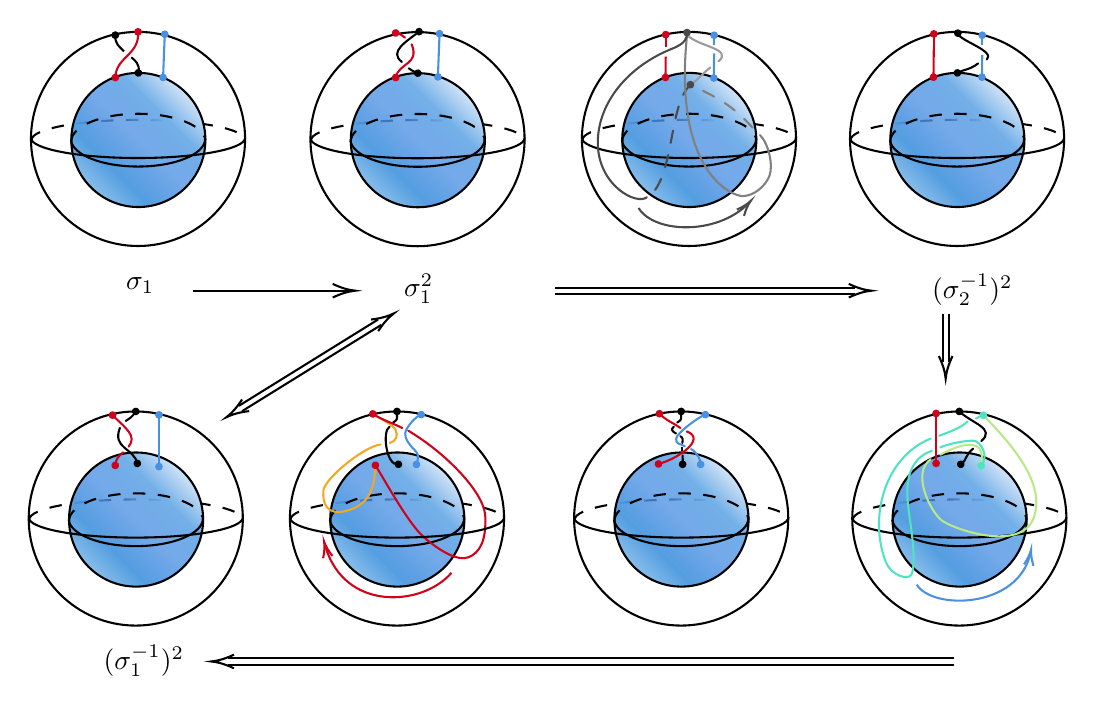
\begin{tikzpicture}[x=0.75pt,y=0.75pt,yscale=-1,xscale=1]
%uncomment if require: \path (0,319); %set diagram left start at 0, and has height of 319

%Shape: Arc [id:dp6282205597384629] 
\draw  [draw opacity=0][dash pattern={on 4.5pt off 4.5pt}] (82.13,54.54) .. controls (82.13,54.47) and (82.12,54.41) .. (82.12,54.34) .. controls (82.12,48.99) and (105.15,44.65) .. (133.56,44.65) .. controls (160.04,44.65) and (181.84,48.42) .. (184.69,53.26) -- (133.56,54.34) -- cycle ; \draw  [dash pattern={on 4.5pt off 4.5pt}] (82.13,54.54) .. controls (82.13,54.47) and (82.12,54.41) .. (82.12,54.34) .. controls (82.12,48.99) and (105.15,44.65) .. (133.56,44.65) .. controls (160.04,44.65) and (181.84,48.42) .. (184.69,53.26) ;  
%Shape: Ellipse [id:dp8895834986117281] 
\path  [shading=_x4b2ox5cs,_nd7rhp6wc,path fading= _8ufflyhw4 ,fading transform={xshift=2}] (101.26,54.34) .. controls (101.26,36.5) and (115.72,22.03) .. (133.56,22.03) .. controls (151.41,22.03) and (165.87,36.5) .. (165.87,54.34) .. controls (165.87,72.18) and (151.41,86.65) .. (133.56,86.65) .. controls (115.72,86.65) and (101.26,72.18) .. (101.26,54.34) -- cycle ; % for fading 
 \draw   (101.26,54.34) .. controls (101.26,36.5) and (115.72,22.03) .. (133.56,22.03) .. controls (151.41,22.03) and (165.87,36.5) .. (165.87,54.34) .. controls (165.87,72.18) and (151.41,86.65) .. (133.56,86.65) .. controls (115.72,86.65) and (101.26,72.18) .. (101.26,54.34) -- cycle ; % for border 

%Shape: Ellipse [id:dp6111171092391365] 
\draw  [color={rgb, 255:red, 0; green, 0; blue, 0 }  ,draw opacity=1 ] (81.84,53.84) .. controls (81.84,25.36) and (104.93,2.26) .. (133.42,2.26) .. controls (161.91,2.26) and (185,25.36) .. (185,53.84) .. controls (185,82.33) and (161.91,105.43) .. (133.42,105.43) .. controls (104.93,105.43) and (81.84,82.33) .. (81.84,53.84) -- cycle ;
%Shape: Arc [id:dp4164707760000881] 
\draw  [draw opacity=0] (165.75,53.72) .. controls (165.75,53.76) and (165.75,53.8) .. (165.75,53.84) .. controls (165.75,61.19) and (151.27,67.15) .. (133.42,67.15) .. controls (116.12,67.15) and (102,61.56) .. (101.13,54.53) -- (133.42,53.84) -- cycle ; \draw   (165.75,53.72) .. controls (165.75,53.76) and (165.75,53.8) .. (165.75,53.84) .. controls (165.75,61.19) and (151.27,67.15) .. (133.42,67.15) .. controls (116.12,67.15) and (102,61.56) .. (101.13,54.53) ;  
%Shape: Arc [id:dp7740913856639409] 
\draw  [draw opacity=0][dash pattern={on 4.5pt off 4.5pt}] (101.26,55.15) .. controls (101.26,55.11) and (101.26,55.06) .. (101.26,55.02) .. controls (101.26,47.67) and (115.73,41.72) .. (133.58,41.72) .. controls (150.88,41.72) and (165.01,47.31) .. (165.87,54.34) -- (133.58,55.02) -- cycle ; \draw  [dash pattern={on 4.5pt off 4.5pt}] (101.26,55.15) .. controls (101.26,55.11) and (101.26,55.06) .. (101.26,55.02) .. controls (101.26,47.67) and (115.73,41.72) .. (133.58,41.72) .. controls (150.88,41.72) and (165.01,47.31) .. (165.87,54.34) ;  
%Shape: Arc [id:dp116926871868964] 
\draw  [draw opacity=0] (184.99,53.15) .. controls (185,53.22) and (185,53.28) .. (185,53.35) .. controls (185,58.7) and (161.9,63.04) .. (133.4,63.04) .. controls (106.86,63.04) and (84.99,59.27) .. (82.12,54.43) -- (133.4,53.35) -- cycle ; \draw   (184.99,53.15) .. controls (185,53.22) and (185,53.28) .. (185,53.35) .. controls (185,58.7) and (161.9,63.04) .. (133.4,63.04) .. controls (106.86,63.04) and (84.99,59.27) .. (82.12,54.43) ;  
%Curve Lines [id:da2450231190260379] 
\draw [color={rgb, 255:red, 208; green, 2; blue, 27 }  ,draw opacity=1 ]   (122.49,24.25) .. controls (122.69,14.23) and (134.29,13.43) .. (133.42,2.26) ;
\draw [shift={(133.42,2.26)}, rotate = 265.56] [color={rgb, 255:red, 208; green, 2; blue, 27 }  ,draw opacity=1 ][fill={rgb, 255:red, 208; green, 2; blue, 27 }  ,fill opacity=1 ][line width=0.75]      (0, 0) circle [x radius= 1.34, y radius= 1.34]   ;
\draw [shift={(122.49,24.25)}, rotate = 271.15] [color={rgb, 255:red, 208; green, 2; blue, 27 }  ,draw opacity=1 ][fill={rgb, 255:red, 208; green, 2; blue, 27 }  ,fill opacity=1 ][line width=0.75]      (0, 0) circle [x radius= 1.34, y radius= 1.34]   ;
%Curve Lines [id:da25147895664806996] 
\draw [color={rgb, 255:red, 0; green, 0; blue, 0 }  ,draw opacity=1 ]   (133.56,22.03) .. controls (134.71,17.65) and (131.48,15.65) .. (130.15,14.54) ;
\draw [shift={(133.56,22.03)}, rotate = 284.61] [color={rgb, 255:red, 0; green, 0; blue, 0 }  ,draw opacity=1 ][fill={rgb, 255:red, 0; green, 0; blue, 0 }  ,fill opacity=1 ][line width=0.75]      (0, 0) circle [x radius= 1.34, y radius= 1.34]   ;
%Straight Lines [id:da9689682157901094] 
\draw [color={rgb, 255:red, 74; green, 144; blue, 226 }  ,draw opacity=1 ]   (146.29,3.43) -- (145.49,24.23) ;
\draw [shift={(145.49,24.23)}, rotate = 92.2] [color={rgb, 255:red, 74; green, 144; blue, 226 }  ,draw opacity=1 ][fill={rgb, 255:red, 74; green, 144; blue, 226 }  ,fill opacity=1 ][line width=0.75]      (0, 0) circle [x radius= 1.34, y radius= 1.34]   ;
\draw [shift={(146.29,3.43)}, rotate = 92.2] [color={rgb, 255:red, 74; green, 144; blue, 226 }  ,draw opacity=1 ][fill={rgb, 255:red, 74; green, 144; blue, 226 }  ,fill opacity=1 ][line width=0.75]      (0, 0) circle [x radius= 1.34, y radius= 1.34]   ;
%Curve Lines [id:da5223663141208712] 
\draw [color={rgb, 255:red, 0; green, 0; blue, 0 }  ,draw opacity=1 ]   (126.71,11.65) .. controls (124.82,9.76) and (122.15,8.21) .. (122.47,3.83) ;
\draw [shift={(122.47,3.83)}, rotate = 274.12] [color={rgb, 255:red, 0; green, 0; blue, 0 }  ,draw opacity=1 ][fill={rgb, 255:red, 0; green, 0; blue, 0 }  ,fill opacity=1 ][line width=0.75]      (0, 0) circle [x radius= 1.34, y radius= 1.34]   ;

%Shape: Arc [id:dp9206463095642927] 
\draw  [draw opacity=0][dash pattern={on 4.5pt off 4.5pt}] (216.79,54.65) .. controls (216.78,54.58) and (216.78,54.52) .. (216.78,54.45) .. controls (216.78,49.1) and (239.81,44.76) .. (268.22,44.76) .. controls (294.69,44.76) and (316.49,48.53) .. (319.35,53.37) -- (268.22,54.45) -- cycle ; \draw  [dash pattern={on 4.5pt off 4.5pt}] (216.79,54.65) .. controls (216.78,54.58) and (216.78,54.52) .. (216.78,54.45) .. controls (216.78,49.1) and (239.81,44.76) .. (268.22,44.76) .. controls (294.69,44.76) and (316.49,48.53) .. (319.35,53.37) ;  
%Shape: Ellipse [id:dp08680266137166615] 
\path  [shading=_vwz4qum48,_yvtms168e,path fading= _9jnbb612z ,fading transform={xshift=2}] (235.91,54.45) .. controls (235.91,36.61) and (250.38,22.15) .. (268.22,22.15) .. controls (286.06,22.15) and (300.53,36.61) .. (300.53,54.45) .. controls (300.53,72.29) and (286.06,86.76) .. (268.22,86.76) .. controls (250.38,86.76) and (235.91,72.29) .. (235.91,54.45) -- cycle ; % for fading 
 \draw   (235.91,54.45) .. controls (235.91,36.61) and (250.38,22.15) .. (268.22,22.15) .. controls (286.06,22.15) and (300.53,36.61) .. (300.53,54.45) .. controls (300.53,72.29) and (286.06,86.76) .. (268.22,86.76) .. controls (250.38,86.76) and (235.91,72.29) .. (235.91,54.45) -- cycle ; % for border 

%Shape: Ellipse [id:dp8720144194883483] 
\draw  [color={rgb, 255:red, 0; green, 0; blue, 0 }  ,draw opacity=1 ] (216.49,53.96) .. controls (216.49,25.47) and (239.59,2.37) .. (268.08,2.37) .. controls (296.57,2.37) and (319.66,25.47) .. (319.66,53.96) .. controls (319.66,82.45) and (296.57,105.54) .. (268.08,105.54) .. controls (239.59,105.54) and (216.49,82.45) .. (216.49,53.96) -- cycle ;
%Shape: Arc [id:dp6390750904664404] 
\draw  [draw opacity=0] (300.4,53.83) .. controls (300.4,53.87) and (300.4,53.92) .. (300.4,53.96) .. controls (300.4,61.31) and (285.93,67.26) .. (268.08,67.26) .. controls (250.78,67.26) and (236.65,61.67) .. (235.79,54.64) -- (268.08,53.96) -- cycle ; \draw   (300.4,53.83) .. controls (300.4,53.87) and (300.4,53.92) .. (300.4,53.96) .. controls (300.4,61.31) and (285.93,67.26) .. (268.08,67.26) .. controls (250.78,67.26) and (236.65,61.67) .. (235.79,54.64) ;  
%Shape: Arc [id:dp11716060403017647] 
\draw  [draw opacity=0][dash pattern={on 4.5pt off 4.5pt}] (235.92,55.26) .. controls (235.91,55.22) and (235.91,55.18) .. (235.91,55.13) .. controls (235.91,47.79) and (250.39,41.83) .. (268.24,41.83) .. controls (285.54,41.83) and (299.66,47.42) .. (300.53,54.45) -- (268.24,55.13) -- cycle ; \draw  [dash pattern={on 4.5pt off 4.5pt}] (235.92,55.26) .. controls (235.91,55.22) and (235.91,55.18) .. (235.91,55.13) .. controls (235.91,47.79) and (250.39,41.83) .. (268.24,41.83) .. controls (285.54,41.83) and (299.66,47.42) .. (300.53,54.45) ;  
%Shape: Arc [id:dp7657597635058822] 
\draw  [draw opacity=0] (319.65,53.26) .. controls (319.66,53.33) and (319.66,53.39) .. (319.66,53.46) .. controls (319.66,58.81) and (296.56,63.15) .. (268.06,63.15) .. controls (241.51,63.15) and (219.65,59.39) .. (216.78,54.54) -- (268.06,53.46) -- cycle ; \draw   (319.65,53.26) .. controls (319.66,53.33) and (319.66,53.39) .. (319.66,53.46) .. controls (319.66,58.81) and (296.56,63.15) .. (268.06,63.15) .. controls (241.51,63.15) and (219.65,59.39) .. (216.78,54.54) ;  
%Curve Lines [id:da5706636066925512] 
\draw [color={rgb, 255:red, 208; green, 2; blue, 27 }  ,draw opacity=1 ][line width=0.75] [line join = round][line cap = round]   (257.54,24.27) .. controls (259.16,16.84) and (269.15,18.29) .. (265.28,8.28) ;
\draw [shift={(257.54,24.27)}, rotate = 282.26] [color={rgb, 255:red, 208; green, 2; blue, 27 }  ,draw opacity=1 ][fill={rgb, 255:red, 208; green, 2; blue, 27 }  ,fill opacity=1 ][line width=0.75] [line join = round][line cap = round]     (0, 0) circle [x radius= 1.34, y radius= 1.34]   ;
%Curve Lines [id:da0372859684656528] 
\draw [color={rgb, 255:red, 208; green, 2; blue, 27 }  ,draw opacity=1 ][line width=0.75] [line join = round][line cap = round]   (257.53,2.79) .. controls (259.79,3.12) and (259.79,3.44) .. (262.05,5.05) ;
\draw [shift={(257.53,2.79)}, rotate = 8.13] [color={rgb, 255:red, 208; green, 2; blue, 27 }  ,draw opacity=1 ][fill={rgb, 255:red, 208; green, 2; blue, 27 }  ,fill opacity=1 ][line width=0.75] [line join = round][line cap = round]     (0, 0) circle [x radius= 1.34, y radius= 1.34]   ;
%Curve Lines [id:da06526178641094971] 
\draw [color={rgb, 255:red, 0; green, 0; blue, 0 }  ,draw opacity=1 ][line width=0.75] [line join = round][line cap = round]   (268.83,2.15) .. controls (262.79,6.9) and (254.04,11.77) .. (260.54,16.77) ;
\draw [shift={(268.83,2.15)}, rotate = 141.82] [color={rgb, 255:red, 0; green, 0; blue, 0 }  ,draw opacity=1 ][fill={rgb, 255:red, 0; green, 0; blue, 0 }  ,fill opacity=1 ][line width=0.75] [line join = round][line cap = round]     (0, 0) circle [x radius= 1.34, y radius= 1.34]   ;
%Curve Lines [id:da6853065147577009] 
\draw [color={rgb, 255:red, 0; green, 0; blue, 0 }  ,draw opacity=1 ][line width=0.75] [line join = round][line cap = round]   (263.82,19.81) .. controls (265.36,20.89) and (266.75,21.66) .. (268.22,22.15) ;
\draw [shift={(268.22,22.15)}, rotate = 18.41] [color={rgb, 255:red, 0; green, 0; blue, 0 }  ,draw opacity=1 ][fill={rgb, 255:red, 0; green, 0; blue, 0 }  ,fill opacity=1 ][line width=0.75] [line join = round][line cap = round]     (0, 0) circle [x radius= 1.34, y radius= 1.34]   ;
%Straight Lines [id:da6772465792684526] 
\draw [color={rgb, 255:red, 74; green, 144; blue, 226 }  ,draw opacity=1 ]   (278.69,3.14) -- (277.89,23.94) ;
\draw [shift={(277.89,23.94)}, rotate = 92.2] [color={rgb, 255:red, 74; green, 144; blue, 226 }  ,draw opacity=1 ][fill={rgb, 255:red, 74; green, 144; blue, 226 }  ,fill opacity=1 ][line width=0.75]      (0, 0) circle [x radius= 1.34, y radius= 1.34]   ;
\draw [shift={(278.69,3.14)}, rotate = 92.2] [color={rgb, 255:red, 74; green, 144; blue, 226 }  ,draw opacity=1 ][fill={rgb, 255:red, 74; green, 144; blue, 226 }  ,fill opacity=1 ][line width=0.75]      (0, 0) circle [x radius= 1.34, y radius= 1.34]   ;

%Shape: Arc [id:dp9669372062427977] 
\draw  [draw opacity=0][dash pattern={on 4.5pt off 4.5pt}] (347.57,54.54) .. controls (347.57,54.47) and (347.56,54.41) .. (347.56,54.34) .. controls (347.56,48.99) and (370.59,44.65) .. (399,44.65) .. controls (425.48,44.65) and (447.28,48.42) .. (450.13,53.26) -- (399,54.34) -- cycle ; \draw  [dash pattern={on 4.5pt off 4.5pt}] (347.57,54.54) .. controls (347.57,54.47) and (347.56,54.41) .. (347.56,54.34) .. controls (347.56,48.99) and (370.59,44.65) .. (399,44.65) .. controls (425.48,44.65) and (447.28,48.42) .. (450.13,53.26) ;  
%Shape: Ellipse [id:dp008634254648815842] 
\path  [shading=_vfr8fvt38,_5s5vn34uc,path fading= _0q53gqdu7 ,fading transform={xshift=2}] (366.7,54.34) .. controls (366.7,36.5) and (381.16,22.03) .. (399,22.03) .. controls (416.85,22.03) and (431.31,36.5) .. (431.31,54.34) .. controls (431.31,72.18) and (416.85,86.65) .. (399,86.65) .. controls (381.16,86.65) and (366.7,72.18) .. (366.7,54.34) -- cycle ; % for fading 
 \draw   (366.7,54.34) .. controls (366.7,36.5) and (381.16,22.03) .. (399,22.03) .. controls (416.85,22.03) and (431.31,36.5) .. (431.31,54.34) .. controls (431.31,72.18) and (416.85,86.65) .. (399,86.65) .. controls (381.16,86.65) and (366.7,72.18) .. (366.7,54.34) -- cycle ; % for border 

%Shape: Ellipse [id:dp5505585043246461] 
\draw  [color={rgb, 255:red, 0; green, 0; blue, 0 }  ,draw opacity=1 ] (347.28,53.84) .. controls (347.28,25.36) and (370.37,2.26) .. (398.86,2.26) .. controls (427.35,2.26) and (450.44,25.36) .. (450.44,53.84) .. controls (450.44,82.33) and (427.35,105.43) .. (398.86,105.43) .. controls (370.37,105.43) and (347.28,82.33) .. (347.28,53.84) -- cycle ;
%Shape: Arc [id:dp030685011817712216] 
\draw  [draw opacity=0] (431.19,53.72) .. controls (431.19,53.76) and (431.19,53.8) .. (431.19,53.84) .. controls (431.19,61.19) and (416.71,67.15) .. (398.86,67.15) .. controls (381.56,67.15) and (367.44,61.56) .. (366.57,54.53) -- (398.86,53.84) -- cycle ; \draw   (431.19,53.72) .. controls (431.19,53.76) and (431.19,53.8) .. (431.19,53.84) .. controls (431.19,61.19) and (416.71,67.15) .. (398.86,67.15) .. controls (381.56,67.15) and (367.44,61.56) .. (366.57,54.53) ;  
%Shape: Arc [id:dp8673619428313148] 
\draw  [draw opacity=0][dash pattern={on 4.5pt off 4.5pt}] (366.7,55.15) .. controls (366.7,55.11) and (366.7,55.06) .. (366.7,55.02) .. controls (366.7,47.67) and (381.17,41.72) .. (399.02,41.72) .. controls (416.32,41.72) and (430.45,47.31) .. (431.31,54.34) -- (399.02,55.02) -- cycle ; \draw  [dash pattern={on 4.5pt off 4.5pt}] (366.7,55.15) .. controls (366.7,55.11) and (366.7,55.06) .. (366.7,55.02) .. controls (366.7,47.67) and (381.17,41.72) .. (399.02,41.72) .. controls (416.32,41.72) and (430.45,47.31) .. (431.31,54.34) ;  
%Shape: Arc [id:dp2483249782885839] 
\draw  [draw opacity=0] (450.43,53.15) .. controls (450.44,53.22) and (450.44,53.28) .. (450.44,53.35) .. controls (450.44,58.7) and (427.34,63.04) .. (398.84,63.04) .. controls (372.3,63.04) and (350.43,59.27) .. (347.56,54.43) -- (398.84,53.35) -- cycle ; \draw   (450.43,53.15) .. controls (450.44,53.22) and (450.44,53.28) .. (450.44,53.35) .. controls (450.44,58.7) and (427.34,63.04) .. (398.84,63.04) .. controls (372.3,63.04) and (350.43,59.27) .. (347.56,54.43) ;  
%Curve Lines [id:da13677975656691022] 
\draw [color={rgb, 255:red, 74; green, 74; blue, 74 }  ,draw opacity=1 ][line width=0.75] [line join = round][line cap = round]   (390.18,10.6) .. controls (367.86,19.71) and (354.02,38.37) .. (354.99,57.43) .. controls (355.95,76.48) and (373.39,85.84) .. (378.56,81.97) ;
%Straight Lines [id:da5910787041087182] 
\draw [color={rgb, 255:red, 208; green, 2; blue, 27 }  ,draw opacity=1 ]   (387.54,24.22) -- (387.66,14.22) ;
\draw [shift={(387.54,24.22)}, rotate = 270.72] [color={rgb, 255:red, 208; green, 2; blue, 27 }  ,draw opacity=1 ][fill={rgb, 255:red, 208; green, 2; blue, 27 }  ,fill opacity=1 ][line width=0.75]      (0, 0) circle [x radius= 1.34, y radius= 1.34]   ;
%Straight Lines [id:da3039712875657117] 
\draw [color={rgb, 255:red, 208; green, 2; blue, 27 }  ,draw opacity=1 ]   (387.66,9.38) -- (387.66,3.59) ;
\draw [shift={(387.66,3.59)}, rotate = 270] [color={rgb, 255:red, 208; green, 2; blue, 27 }  ,draw opacity=1 ][fill={rgb, 255:red, 208; green, 2; blue, 27 }  ,fill opacity=1 ][line width=0.75]      (0, 0) circle [x radius= 1.34, y radius= 1.34]   ;
%Curve Lines [id:da13005280298726696] 
\draw [color={rgb, 255:red, 128; green, 128; blue, 128 }  ,draw opacity=1 ][line width=0.75] [line join = round][line cap = round] [dash pattern={on 4.5pt off 4.5pt}]  (429.54,48.45) .. controls (417.91,35.54) and (409.19,32.63) .. (399.55,27.72) ;
%Curve Lines [id:da8611148227503174] 
\draw [color={rgb, 255:red, 155; green, 155; blue, 155 }  ,draw opacity=1 ][line width=0.75] [line join = round][line cap = round]   (397.93,3.82) .. controls (404.07,9.63) and (420.17,10.35) .. (413.07,16.48) ;
%Curve Lines [id:da7314247219037404] 
\draw [color={rgb, 255:red, 155; green, 155; blue, 155 }  ,draw opacity=1 ][line width=0.75] [line join = round][line cap = round]   (399.55,27.72) .. controls (402.53,26.02) and (405,22.62) .. (409.19,19.39) ;
%Straight Lines [id:da37050607501791477] 
\draw [color={rgb, 255:red, 74; green, 144; blue, 226 }  ,draw opacity=1 ]   (410.84,24.47) -- (410.97,12.61) ;
\draw [shift={(410.84,24.47)}, rotate = 270.6] [color={rgb, 255:red, 74; green, 144; blue, 226 }  ,draw opacity=1 ][fill={rgb, 255:red, 74; green, 144; blue, 226 }  ,fill opacity=1 ][line width=0.75]      (0, 0) circle [x radius= 1.34, y radius= 1.34]   ;
%Straight Lines [id:da08001827523500515] 
\draw [color={rgb, 255:red, 74; green, 144; blue, 226 }  ,draw opacity=1 ]   (410.97,8.73) -- (410.97,3.89) ;
\draw [shift={(410.97,3.89)}, rotate = 270] [color={rgb, 255:red, 74; green, 144; blue, 226 }  ,draw opacity=1 ][fill={rgb, 255:red, 74; green, 144; blue, 226 }  ,fill opacity=1 ][line width=0.75]      (0, 0) circle [x radius= 1.34, y radius= 1.34]   ;
%Curve Lines [id:da08052341557121045] 
\draw [color={rgb, 255:red, 74; green, 74; blue, 74 }  ,draw opacity=1 ][line width=0.75] [line join = round][line cap = round] [dash pattern={on 4.5pt off 4.5pt}]  (399.55,27.72) .. controls (389.54,37.08) and (391.8,67.11) .. (381.79,79.39) ;
\draw [shift={(399.55,27.72)}, rotate = 136.91] [color={rgb, 255:red, 74; green, 74; blue, 74 }  ,draw opacity=1 ][fill={rgb, 255:red, 74; green, 74; blue, 74 }  ,fill opacity=1 ][line width=0.75] [line join = round][line cap = round]     (0, 0) circle [x radius= 1.34, y radius= 1.34]   ;
%Curve Lines [id:da8760765644978001] 
\draw [color={rgb, 255:red, 128; green, 128; blue, 128 }  ,draw opacity=1 ][line width=0.75] [line join = round][line cap = round]   (397.93,3.82) .. controls (391.11,69.44) and (419.53,81.71) .. (425.02,81.39) .. controls (430.51,81.07) and (435.67,76.55) .. (437.61,71.7) .. controls (439.55,66.86) and (437.36,56.27) .. (433.09,52) ;
%Curve Lines [id:da9250196330646012] 
\draw [color={rgb, 255:red, 74; green, 74; blue, 74 }  ,draw opacity=1 ][line width=0.75] [line join = round][line cap = round]   (397.91,2.59) .. controls (397.91,5.17) and (397.57,7.76) .. (390.18,10.6) ;
\draw [shift={(397.91,2.59)}, rotate = 90] [color={rgb, 255:red, 74; green, 74; blue, 74 }  ,draw opacity=1 ][fill={rgb, 255:red, 74; green, 74; blue, 74 }  ,fill opacity=1 ][line width=0.75] [line join = round][line cap = round]     (0, 0) circle [x radius= 1.34, y radius= 1.34]   ;
%Curve Lines [id:da5707590126364628] 
\draw [color={rgb, 255:red, 74; green, 74; blue, 74 }  ,draw opacity=1 ]   (374.58,87.13) .. controls (382.15,99.4) and (412.25,100.28) .. (427.31,85.09) ;
\draw [shift={(428.67,83.64)}, rotate = 131.05] [color={rgb, 255:red, 74; green, 74; blue, 74 }  ,draw opacity=1 ][line width=0.75]    (7.65,-2.3) .. controls (4.86,-0.97) and (2.31,-0.21) .. (0,0) .. controls (2.31,0.21) and (4.86,0.98) .. (7.65,2.3)   ;

%Shape: Arc [id:dp5783810318119713] 
\draw  [draw opacity=0][dash pattern={on 4.5pt off 4.5pt}] (476.74,54.54) .. controls (476.73,54.47) and (476.73,54.41) .. (476.73,54.34) .. controls (476.73,48.99) and (499.76,44.65) .. (528.17,44.65) .. controls (554.64,44.65) and (576.45,48.42) .. (579.3,53.26) -- (528.17,54.34) -- cycle ; \draw  [dash pattern={on 4.5pt off 4.5pt}] (476.74,54.54) .. controls (476.73,54.47) and (476.73,54.41) .. (476.73,54.34) .. controls (476.73,48.99) and (499.76,44.65) .. (528.17,44.65) .. controls (554.64,44.65) and (576.45,48.42) .. (579.3,53.26) ;  
%Shape: Ellipse [id:dp6935822155155171] 
\path  [shading=_zq6gr1ktq,_t602pfluu,path fading= _tfgy5szke ,fading transform={xshift=2}] (495.86,54.34) .. controls (495.86,36.5) and (510.33,22.03) .. (528.17,22.03) .. controls (546.01,22.03) and (560.48,36.5) .. (560.48,54.34) .. controls (560.48,72.18) and (546.01,86.65) .. (528.17,86.65) .. controls (510.33,86.65) and (495.86,72.18) .. (495.86,54.34) -- cycle ; % for fading 
 \draw   (495.86,54.34) .. controls (495.86,36.5) and (510.33,22.03) .. (528.17,22.03) .. controls (546.01,22.03) and (560.48,36.5) .. (560.48,54.34) .. controls (560.48,72.18) and (546.01,86.65) .. (528.17,86.65) .. controls (510.33,86.65) and (495.86,72.18) .. (495.86,54.34) -- cycle ; % for border 

%Shape: Ellipse [id:dp7138862104028538] 
\draw  [color={rgb, 255:red, 0; green, 0; blue, 0 }  ,draw opacity=1 ] (476.44,53.84) .. controls (476.44,25.36) and (499.54,2.26) .. (528.03,2.26) .. controls (556.52,2.26) and (579.61,25.36) .. (579.61,53.84) .. controls (579.61,82.33) and (556.52,105.43) .. (528.03,105.43) .. controls (499.54,105.43) and (476.44,82.33) .. (476.44,53.84) -- cycle ;
%Shape: Arc [id:dp3289496095270341] 
\draw  [draw opacity=0] (560.35,53.72) .. controls (560.35,53.76) and (560.35,53.8) .. (560.35,53.84) .. controls (560.35,61.19) and (545.88,67.15) .. (528.03,67.15) .. controls (510.73,67.15) and (496.6,61.56) .. (495.74,54.53) -- (528.03,53.84) -- cycle ; \draw   (560.35,53.72) .. controls (560.35,53.76) and (560.35,53.8) .. (560.35,53.84) .. controls (560.35,61.19) and (545.88,67.15) .. (528.03,67.15) .. controls (510.73,67.15) and (496.6,61.56) .. (495.74,54.53) ;  
%Shape: Arc [id:dp767271179059482] 
\draw  [draw opacity=0][dash pattern={on 4.5pt off 4.5pt}] (495.87,55.15) .. controls (495.86,55.11) and (495.86,55.06) .. (495.86,55.02) .. controls (495.86,47.67) and (510.34,41.72) .. (528.19,41.72) .. controls (545.49,41.72) and (559.61,47.31) .. (560.48,54.34) -- (528.19,55.02) -- cycle ; \draw  [dash pattern={on 4.5pt off 4.5pt}] (495.87,55.15) .. controls (495.86,55.11) and (495.86,55.06) .. (495.86,55.02) .. controls (495.86,47.67) and (510.34,41.72) .. (528.19,41.72) .. controls (545.49,41.72) and (559.61,47.31) .. (560.48,54.34) ;  
%Shape: Arc [id:dp2821452433255107] 
\draw  [draw opacity=0] (579.6,53.15) .. controls (579.61,53.22) and (579.61,53.28) .. (579.61,53.35) .. controls (579.61,58.7) and (556.51,63.04) .. (528.01,63.04) .. controls (501.46,63.04) and (479.6,59.27) .. (476.73,54.43) -- (528.01,53.35) -- cycle ; \draw   (579.6,53.15) .. controls (579.61,53.22) and (579.61,53.28) .. (579.61,53.35) .. controls (579.61,58.7) and (556.51,63.04) .. (528.01,63.04) .. controls (501.46,63.04) and (479.6,59.27) .. (476.73,54.43) ;  
%Straight Lines [id:da7838481985878138] 
\draw [color={rgb, 255:red, 208; green, 2; blue, 27 }  ,draw opacity=1 ]   (516.66,24.09) -- (516.83,9.38) ;
\draw [shift={(516.66,24.09)}, rotate = 270.68] [color={rgb, 255:red, 208; green, 2; blue, 27 }  ,draw opacity=1 ][fill={rgb, 255:red, 208; green, 2; blue, 27 }  ,fill opacity=1 ][line width=0.75]      (0, 0) circle [x radius= 1.34, y radius= 1.34]   ;
%Straight Lines [id:da140994506205246] 
\draw [color={rgb, 255:red, 208; green, 2; blue, 27 }  ,draw opacity=1 ]   (516.83,9.38) -- (516.83,3.24) ;
\draw [shift={(516.83,3.24)}, rotate = 270] [color={rgb, 255:red, 208; green, 2; blue, 27 }  ,draw opacity=1 ][fill={rgb, 255:red, 208; green, 2; blue, 27 }  ,fill opacity=1 ][line width=0.75]      (0, 0) circle [x radius= 1.34, y radius= 1.34]   ;
%Curve Lines [id:da9314111484035377] 
\draw [color={rgb, 255:red, 0; green, 0; blue, 0 }  ,draw opacity=1 ][line width=0.75] [line join = round][line cap = round]   (528.4,2.89) .. controls (528.41,6.22) and (546.78,11.47) .. (542.41,15.59) ;
\draw [shift={(528.4,2.89)}, rotate = 89.9] [color={rgb, 255:red, 0; green, 0; blue, 0 }  ,draw opacity=1 ][fill={rgb, 255:red, 0; green, 0; blue, 0 }  ,fill opacity=1 ][line width=0.75] [line join = round][line cap = round]     (0, 0) circle [x radius= 1.34, y radius= 1.34]   ;
%Curve Lines [id:da18502436820817203] 
\draw [color={rgb, 255:red, 0; green, 0; blue, 0 }  ,draw opacity=1 ][line width=0.75] [line join = round][line cap = round]   (528.17,22.03) .. controls (531.15,20.33) and (533.96,20.7) .. (538.16,17.47) ;
\draw [shift={(528.17,22.03)}, rotate = 330.26] [color={rgb, 255:red, 0; green, 0; blue, 0 }  ,draw opacity=1 ][fill={rgb, 255:red, 0; green, 0; blue, 0 }  ,fill opacity=1 ][line width=0.75] [line join = round][line cap = round]     (0, 0) circle [x radius= 1.34, y radius= 1.34]   ;
%Straight Lines [id:da15856837189261697] 
\draw [color={rgb, 255:red, 74; green, 144; blue, 226 }  ,draw opacity=1 ]   (540.03,24.09) -- (540.16,13.47) ;
\draw [shift={(540.03,24.09)}, rotate = 270.67] [color={rgb, 255:red, 74; green, 144; blue, 226 }  ,draw opacity=1 ][fill={rgb, 255:red, 74; green, 144; blue, 226 }  ,fill opacity=1 ][line width=0.75]      (0, 0) circle [x radius= 1.34, y radius= 1.34]   ;
%Straight Lines [id:da25035384663554416] 
\draw [color={rgb, 255:red, 74; green, 144; blue, 226 }  ,draw opacity=1 ]   (540.14,8.73) -- (540.14,3.89) ;
\draw [shift={(540.14,3.89)}, rotate = 270] [color={rgb, 255:red, 74; green, 144; blue, 226 }  ,draw opacity=1 ][fill={rgb, 255:red, 74; green, 144; blue, 226 }  ,fill opacity=1 ][line width=0.75]      (0, 0) circle [x radius= 1.34, y radius= 1.34]   ;

%Shape: Arc [id:dp2193480814229003] 
\draw  [draw opacity=0][dash pattern={on 4.5pt off 4.5pt}] (477.83,237.42) .. controls (477.82,237.35) and (477.82,237.29) .. (477.82,237.22) .. controls (477.82,231.87) and (500.85,227.53) .. (529.26,227.53) .. controls (555.73,227.53) and (577.53,231.3) .. (580.39,236.14) -- (529.26,237.22) -- cycle ; \draw  [dash pattern={on 4.5pt off 4.5pt}] (477.83,237.42) .. controls (477.82,237.35) and (477.82,237.29) .. (477.82,237.22) .. controls (477.82,231.87) and (500.85,227.53) .. (529.26,227.53) .. controls (555.73,227.53) and (577.53,231.3) .. (580.39,236.14) ;  
%Shape: Ellipse [id:dp9513847917634946] 
\path  [shading=_p3n07yvia,_tdpxlbu31,path fading= _cgc6bj5u2 ,fading transform={xshift=2}] (496.95,237.22) .. controls (496.95,219.38) and (511.42,204.91) .. (529.26,204.91) .. controls (547.1,204.91) and (561.57,219.38) .. (561.57,237.22) .. controls (561.57,255.06) and (547.1,269.53) .. (529.26,269.53) .. controls (511.42,269.53) and (496.95,255.06) .. (496.95,237.22) -- cycle ; % for fading 
 \draw   (496.95,237.22) .. controls (496.95,219.38) and (511.42,204.91) .. (529.26,204.91) .. controls (547.1,204.91) and (561.57,219.38) .. (561.57,237.22) .. controls (561.57,255.06) and (547.1,269.53) .. (529.26,269.53) .. controls (511.42,269.53) and (496.95,255.06) .. (496.95,237.22) -- cycle ; % for border 

%Shape: Ellipse [id:dp11450717923244902] 
\draw  [color={rgb, 255:red, 0; green, 0; blue, 0 }  ,draw opacity=1 ] (477.53,236.72) .. controls (477.53,208.23) and (500.63,185.14) .. (529.12,185.14) .. controls (557.61,185.14) and (580.7,208.23) .. (580.7,236.72) .. controls (580.7,265.21) and (557.61,288.31) .. (529.12,288.31) .. controls (500.63,288.31) and (477.53,265.21) .. (477.53,236.72) -- cycle ;
%Shape: Arc [id:dp8786473340348733] 
\draw  [draw opacity=0] (561.44,236.6) .. controls (561.44,236.64) and (561.44,236.68) .. (561.44,236.72) .. controls (561.44,244.07) and (546.97,250.03) .. (529.12,250.03) .. controls (511.82,250.03) and (497.69,244.44) .. (496.83,237.41) -- (529.12,236.72) -- cycle ; \draw   (561.44,236.6) .. controls (561.44,236.64) and (561.44,236.68) .. (561.44,236.72) .. controls (561.44,244.07) and (546.97,250.03) .. (529.12,250.03) .. controls (511.82,250.03) and (497.69,244.44) .. (496.83,237.41) ;  
%Shape: Arc [id:dp297427975389128] 
\draw  [draw opacity=0][dash pattern={on 4.5pt off 4.5pt}] (496.96,238.03) .. controls (496.95,237.98) and (496.95,237.94) .. (496.95,237.9) .. controls (496.95,230.55) and (511.43,224.6) .. (529.28,224.6) .. controls (546.58,224.6) and (560.7,230.19) .. (561.57,237.22) -- (529.28,237.9) -- cycle ; \draw  [dash pattern={on 4.5pt off 4.5pt}] (496.96,238.03) .. controls (496.95,237.98) and (496.95,237.94) .. (496.95,237.9) .. controls (496.95,230.55) and (511.43,224.6) .. (529.28,224.6) .. controls (546.58,224.6) and (560.7,230.19) .. (561.57,237.22) ;  
%Shape: Arc [id:dp6512740899097842] 
\draw  [draw opacity=0] (580.69,236.03) .. controls (580.7,236.1) and (580.7,236.16) .. (580.7,236.23) .. controls (580.7,241.58) and (557.6,245.92) .. (529.1,245.92) .. controls (502.55,245.92) and (480.69,242.15) .. (477.82,237.31) -- (529.1,236.23) -- cycle ; \draw   (580.69,236.03) .. controls (580.7,236.1) and (580.7,236.16) .. (580.7,236.23) .. controls (580.7,241.58) and (557.6,245.92) .. (529.1,245.92) .. controls (502.55,245.92) and (480.69,242.15) .. (477.82,237.31) ;  
%Straight Lines [id:da010972011984689445] 
\draw [color={rgb, 255:red, 208; green, 2; blue, 27 }  ,draw opacity=1 ]   (517.92,210.17) -- (517.92,192.26) ;
\draw [shift={(517.92,210.17)}, rotate = 270] [color={rgb, 255:red, 208; green, 2; blue, 27 }  ,draw opacity=1 ][fill={rgb, 255:red, 208; green, 2; blue, 27 }  ,fill opacity=1 ][line width=0.75]      (0, 0) circle [x radius= 1.34, y radius= 1.34]   ;
%Straight Lines [id:da2417870283015502] 
\draw [color={rgb, 255:red, 208; green, 2; blue, 27 }  ,draw opacity=1 ]   (517.92,192.26) -- (517.92,186.12) ;
\draw [shift={(517.92,186.12)}, rotate = 270] [color={rgb, 255:red, 208; green, 2; blue, 27 }  ,draw opacity=1 ][fill={rgb, 255:red, 208; green, 2; blue, 27 }  ,fill opacity=1 ][line width=0.75]      (0, 0) circle [x radius= 1.34, y radius= 1.34]   ;
%Curve Lines [id:da14399982801112743] 
\draw [color={rgb, 255:red, 0; green, 0; blue, 0 }  ,draw opacity=1 ][line width=0.75] [line join = round][line cap = round]   (529.12,185.14) .. controls (535.25,190.95) and (546.78,193.33) .. (539.67,199.47) ;
\draw [shift={(529.12,185.14)}, rotate = 43.45] [color={rgb, 255:red, 0; green, 0; blue, 0 }  ,draw opacity=1 ][fill={rgb, 255:red, 0; green, 0; blue, 0 }  ,fill opacity=1 ][line width=0.75] [line join = round][line cap = round]     (0, 0) circle [x radius= 1.34, y radius= 1.34]   ;
%Curve Lines [id:da8834595657290718] 
\draw [color={rgb, 255:red, 0; green, 0; blue, 0 }  ,draw opacity=1 ][line width=0.75] [line join = round][line cap = round]   (529.81,210.6) .. controls (532.79,208.89) and (531.6,206.28) .. (535.79,203.05) ;
\draw [shift={(529.81,210.6)}, rotate = 330.26] [color={rgb, 255:red, 0; green, 0; blue, 0 }  ,draw opacity=1 ][fill={rgb, 255:red, 0; green, 0; blue, 0 }  ,fill opacity=1 ][line width=0.75] [line join = round][line cap = round]     (0, 0) circle [x radius= 1.34, y radius= 1.34]   ;
%Curve Lines [id:da21316146124189128] 
\draw [color={rgb, 255:red, 80; green, 227; blue, 194 }  ,draw opacity=1 ][line width=0.75] [line join = round][line cap = round]   (533.1,189.86) .. controls (530.41,193.09) and (522.07,195.78) .. (519.38,196.86) ;
%Curve Lines [id:da3497508229683557] 
\draw [color={rgb, 255:red, 80; green, 227; blue, 194 }  ,draw opacity=1 ][line width=0.75] [line join = round][line cap = round]   (515.34,198.2) .. controls (492.95,207.16) and (485.25,236.54) .. (493.82,257.94) .. controls (496.31,264.19) and (504.58,266.56) .. (505.99,263.78) ;
%Curve Lines [id:da5159968039962499] 
\draw [color={rgb, 255:red, 80; green, 227; blue, 194 }  ,draw opacity=1 ][line width=0.75] [line join = round][line cap = round]   (505.99,263.78) .. controls (508.88,257.94) and (505.39,238.84) .. (504.85,233.73) .. controls (504.31,228.61) and (500.54,209.24) .. (515.88,204.12) ;
%Curve Lines [id:da3595287211271989] 
\draw [color={rgb, 255:red, 184; green, 233; blue, 134 }  ,draw opacity=1 ][line width=0.75] [line join = round][line cap = round]   (519.92,206.01) .. controls (531.22,199.82) and (542.25,197.67) .. (539.62,211.31) ;
%Curve Lines [id:da12919854792020558] 
\draw [color={rgb, 255:red, 184; green, 233; blue, 134 }  ,draw opacity=1 ][line width=0.75] [line join = round][line cap = round]   (540.7,186.96) .. controls (551.48,198.27) and (571,218.24) .. (565.13,235.88) .. controls (559.25,253.51) and (525.84,241.8) .. (520.46,237.49) .. controls (515.07,233.19) and (505.92,214.62) .. (515.34,208.16) ;
%Curve Lines [id:da5371296352684112] 
\draw [color={rgb, 255:red, 80; green, 227; blue, 194 }  ,draw opacity=1 ][line width=0.75] [line join = round][line cap = round]   (519.92,202.51) .. controls (522.55,200.97) and (533.2,198.81) .. (536.33,199.28) .. controls (539.46,199.75) and (543.6,206.55) .. (539.62,211.31) ;
\draw [shift={(539.62,211.31)}, rotate = 129.84] [color={rgb, 255:red, 80; green, 227; blue, 194 }  ,draw opacity=1 ][fill={rgb, 255:red, 80; green, 227; blue, 194 }  ,fill opacity=1 ][line width=0.75] [line join = round][line cap = round]     (0, 0) circle [x radius= 1.34, y radius= 1.34]   ;
%Curve Lines [id:da9552466106127524] 
\draw [color={rgb, 255:red, 80; green, 227; blue, 194 }  ,draw opacity=1 ][line width=0.75] [line join = round][line cap = round]   (540.7,186.96) .. controls (539.68,186.96) and (538.29,188.16) .. (537.07,188.57) ;
\draw [shift={(540.7,186.96)}, rotate = 180] [color={rgb, 255:red, 80; green, 227; blue, 194 }  ,draw opacity=1 ][fill={rgb, 255:red, 80; green, 227; blue, 194 }  ,fill opacity=1 ][line width=0.75] [line join = round][line cap = round]     (0, 0) circle [x radius= 1.34, y radius= 1.34]   ;

%Shape: Arc [id:dp958020378956921] 
\draw  [draw opacity=0][dash pattern={on 4.5pt off 4.5pt}] (343.82,237.42) .. controls (343.81,237.35) and (343.81,237.29) .. (343.81,237.22) .. controls (343.81,231.87) and (366.84,227.53) .. (395.25,227.53) .. controls (421.72,227.53) and (443.52,231.3) .. (446.37,236.14) -- (395.25,237.22) -- cycle ; \draw  [dash pattern={on 4.5pt off 4.5pt}] (343.82,237.42) .. controls (343.81,237.35) and (343.81,237.29) .. (343.81,237.22) .. controls (343.81,231.87) and (366.84,227.53) .. (395.25,227.53) .. controls (421.72,227.53) and (443.52,231.3) .. (446.37,236.14) ;  
%Shape: Ellipse [id:dp8891684768888104] 
\path  [shading=_yi08ue4qu,_ljnt52mjn,path fading= _x12ux2416 ,fading transform={xshift=2}] (362.94,237.22) .. controls (362.94,219.38) and (377.41,204.91) .. (395.25,204.91) .. controls (413.09,204.91) and (427.56,219.38) .. (427.56,237.22) .. controls (427.56,255.06) and (413.09,269.53) .. (395.25,269.53) .. controls (377.41,269.53) and (362.94,255.06) .. (362.94,237.22) -- cycle ; % for fading 
 \draw   (362.94,237.22) .. controls (362.94,219.38) and (377.41,204.91) .. (395.25,204.91) .. controls (413.09,204.91) and (427.56,219.38) .. (427.56,237.22) .. controls (427.56,255.06) and (413.09,269.53) .. (395.25,269.53) .. controls (377.41,269.53) and (362.94,255.06) .. (362.94,237.22) -- cycle ; % for border 

%Shape: Ellipse [id:dp6664207859337201] 
\draw  [color={rgb, 255:red, 0; green, 0; blue, 0 }  ,draw opacity=1 ] (343.52,236.72) .. controls (343.52,208.23) and (366.62,185.14) .. (395.11,185.14) .. controls (423.59,185.14) and (446.69,208.23) .. (446.69,236.72) .. controls (446.69,265.21) and (423.59,288.31) .. (395.11,288.31) .. controls (366.62,288.31) and (343.52,265.21) .. (343.52,236.72) -- cycle ;
%Shape: Arc [id:dp13127844437500258] 
\draw  [draw opacity=0] (427.43,236.6) .. controls (427.43,236.64) and (427.43,236.68) .. (427.43,236.72) .. controls (427.43,244.07) and (412.96,250.03) .. (395.11,250.03) .. controls (377.81,250.03) and (363.68,244.44) .. (362.82,237.41) -- (395.11,236.72) -- cycle ; \draw   (427.43,236.6) .. controls (427.43,236.64) and (427.43,236.68) .. (427.43,236.72) .. controls (427.43,244.07) and (412.96,250.03) .. (395.11,250.03) .. controls (377.81,250.03) and (363.68,244.44) .. (362.82,237.41) ;  
%Shape: Arc [id:dp16432686199719182] 
\draw  [draw opacity=0][dash pattern={on 4.5pt off 4.5pt}] (362.94,238.03) .. controls (362.94,237.98) and (362.94,237.94) .. (362.94,237.9) .. controls (362.94,230.55) and (377.42,224.6) .. (395.27,224.6) .. controls (412.57,224.6) and (426.69,230.19) .. (427.56,237.22) -- (395.27,237.9) -- cycle ; \draw  [dash pattern={on 4.5pt off 4.5pt}] (362.94,238.03) .. controls (362.94,237.98) and (362.94,237.94) .. (362.94,237.9) .. controls (362.94,230.55) and (377.42,224.6) .. (395.27,224.6) .. controls (412.57,224.6) and (426.69,230.19) .. (427.56,237.22) ;  
%Shape: Arc [id:dp49137717031547856] 
\draw  [draw opacity=0] (446.68,236.03) .. controls (446.69,236.1) and (446.69,236.16) .. (446.69,236.23) .. controls (446.69,241.58) and (423.59,245.92) .. (395.09,245.92) .. controls (368.54,245.92) and (346.68,242.15) .. (343.81,237.31) -- (395.09,236.23) -- cycle ; \draw   (446.68,236.03) .. controls (446.69,236.1) and (446.69,236.16) .. (446.69,236.23) .. controls (446.69,241.58) and (423.59,245.92) .. (395.09,245.92) .. controls (368.54,245.92) and (346.68,242.15) .. (343.81,237.31) ;  
%Curve Lines [id:da3639181903311217] 
\draw [color={rgb, 255:red, 0; green, 0; blue, 0 }  ,draw opacity=1 ][line width=0.75] [line join = round][line cap = round]   (395.11,185.14) .. controls (394.96,188.76) and (395.84,188.9) .. (393.2,190.52) ;
\draw [shift={(395.11,185.14)}, rotate = 92.29] [color={rgb, 255:red, 0; green, 0; blue, 0 }  ,draw opacity=1 ][fill={rgb, 255:red, 0; green, 0; blue, 0 }  ,fill opacity=1 ][line width=0.75] [line join = round][line cap = round]     (0, 0) circle [x radius= 1.34, y radius= 1.34]   ;
%Curve Lines [id:da015182272999871627] 
\draw [color={rgb, 255:red, 0; green, 0; blue, 0 }  ,draw opacity=1 ][line width=0.75] [line join = round][line cap = round]   (395.79,210.6) .. controls (395.69,206.98) and (395.94,212.92) .. (395.82,206.31) ;
\draw [shift={(395.79,210.6)}, rotate = 268.39] [color={rgb, 255:red, 0; green, 0; blue, 0 }  ,draw opacity=1 ][fill={rgb, 255:red, 0; green, 0; blue, 0 }  ,fill opacity=1 ][line width=0.75] [line join = round][line cap = round]     (0, 0) circle [x radius= 1.34, y radius= 1.34]   ;
%Curve Lines [id:da6128985593923537] 
\draw [color={rgb, 255:red, 208; green, 2; blue, 27 }  ,draw opacity=1 ][line width=0.75] [line join = round][line cap = round]   (384.16,210.44) .. controls (393.15,208.13) and (407.69,198.44) .. (397.77,194.75) ;
\draw [shift={(384.16,210.44)}, rotate = 345.62] [color={rgb, 255:red, 208; green, 2; blue, 27 }  ,draw opacity=1 ][fill={rgb, 255:red, 208; green, 2; blue, 27 }  ,fill opacity=1 ][line width=0.75] [line join = round][line cap = round]     (0, 0) circle [x radius= 1.34, y radius= 1.34]   ;
%Curve Lines [id:da7847888878963316] 
\draw [color={rgb, 255:red, 208; green, 2; blue, 27 }  ,draw opacity=1 ][line width=0.75] [line join = round][line cap = round]   (384.62,186.22) .. controls (388.08,189.68) and (391.31,190.6) .. (394.77,193.14) ;
\draw [shift={(384.62,186.22)}, rotate = 45] [color={rgb, 255:red, 208; green, 2; blue, 27 }  ,draw opacity=1 ][fill={rgb, 255:red, 208; green, 2; blue, 27 }  ,fill opacity=1 ][line width=0.75] [line join = round][line cap = round]     (0, 0) circle [x radius= 1.34, y radius= 1.34]   ;
%Curve Lines [id:da036054893039886515] 
\draw [color={rgb, 255:red, 74; green, 144; blue, 226 }  ,draw opacity=1 ][line width=0.75] [line join = round][line cap = round]   (406.76,186.68) .. controls (404.36,187.23) and (392.92,195.44) .. (392.69,198.21) .. controls (392.46,200.98) and (394.31,200.52) .. (396.85,201.9) ;
\draw [shift={(406.76,186.68)}, rotate = 167] [color={rgb, 255:red, 74; green, 144; blue, 226 }  ,draw opacity=1 ][fill={rgb, 255:red, 74; green, 144; blue, 226 }  ,fill opacity=1 ][line width=0.75] [line join = round][line cap = round]     (0, 0) circle [x radius= 1.34, y radius= 1.34]   ;
%Curve Lines [id:da4160151088774431] 
\draw [color={rgb, 255:red, 74; green, 144; blue, 226 }  ,draw opacity=1 ][line width=0.75] [line join = round][line cap = round]   (399.84,203.29) .. controls (402.61,204.44) and (404.81,209.27) .. (404.46,210.67) ;
\draw [shift={(404.46,210.67)}, rotate = 104.04] [color={rgb, 255:red, 74; green, 144; blue, 226 }  ,draw opacity=1 ][fill={rgb, 255:red, 74; green, 144; blue, 226 }  ,fill opacity=1 ][line width=0.75] [line join = round][line cap = round]     (0, 0) circle [x radius= 1.34, y radius= 1.34]   ;
%Curve Lines [id:da6153240198054679] 
\draw [color={rgb, 255:red, 0; green, 0; blue, 0 }  ,draw opacity=1 ][line width=0.75] [line join = round][line cap = round]   (394.67,196.98) .. controls (396.28,198.3) and (395.84,198.59) .. (395.69,200.29) ;
%Straight Lines [id:da6356863180517809] 
\draw    (395.69,202.31) -- (395.69,204.01) ;
%Curve Lines [id:da43862704161491073] 
\draw [color={rgb, 255:red, 0; green, 0; blue, 0 }  ,draw opacity=1 ][line width=0.75] [line join = round][line cap = round]   (391.59,192.43) .. controls (389.97,193.75) and (390.7,194.78) .. (392.61,195.74) ;
%Shape: Arc [id:dp5633147847686892] 
\draw  [draw opacity=0][dash pattern={on 4.5pt off 4.5pt}] (206.9,237.42) .. controls (206.89,237.35) and (206.89,237.29) .. (206.89,237.22) .. controls (206.89,231.87) and (229.92,227.53) .. (258.33,227.53) .. controls (284.8,227.53) and (306.61,231.3) .. (309.46,236.14) -- (258.33,237.22) -- cycle ; \draw  [dash pattern={on 4.5pt off 4.5pt}] (206.9,237.42) .. controls (206.89,237.35) and (206.89,237.29) .. (206.89,237.22) .. controls (206.89,231.87) and (229.92,227.53) .. (258.33,227.53) .. controls (284.8,227.53) and (306.61,231.3) .. (309.46,236.14) ;  
%Shape: Ellipse [id:dp6026839103228829] 
\path  [shading=_56eryxytu,_xctq6wp81,path fading= _2vmw315b0 ,fading transform={xshift=2}] (226.03,237.22) .. controls (226.03,219.38) and (240.49,204.91) .. (258.33,204.91) .. controls (276.17,204.91) and (290.64,219.38) .. (290.64,237.22) .. controls (290.64,255.06) and (276.17,269.53) .. (258.33,269.53) .. controls (240.49,269.53) and (226.03,255.06) .. (226.03,237.22) -- cycle ; % for fading 
 \draw   (226.03,237.22) .. controls (226.03,219.38) and (240.49,204.91) .. (258.33,204.91) .. controls (276.17,204.91) and (290.64,219.38) .. (290.64,237.22) .. controls (290.64,255.06) and (276.17,269.53) .. (258.33,269.53) .. controls (240.49,269.53) and (226.03,255.06) .. (226.03,237.22) -- cycle ; % for border 

%Shape: Ellipse [id:dp7578611115444678] 
\draw  [color={rgb, 255:red, 0; green, 0; blue, 0 }  ,draw opacity=1 ] (206.6,236.72) .. controls (206.6,208.23) and (229.7,185.14) .. (258.19,185.14) .. controls (286.68,185.14) and (309.77,208.23) .. (309.77,236.72) .. controls (309.77,265.21) and (286.68,288.31) .. (258.19,288.31) .. controls (229.7,288.31) and (206.6,265.21) .. (206.6,236.72) -- cycle ;
%Shape: Arc [id:dp8434450103204563] 
\draw  [draw opacity=0] (290.51,236.6) .. controls (290.51,236.64) and (290.52,236.68) .. (290.52,236.72) .. controls (290.52,244.07) and (276.04,250.03) .. (258.19,250.03) .. controls (240.89,250.03) and (226.76,244.44) .. (225.9,237.41) -- (258.19,236.72) -- cycle ; \draw   (290.51,236.6) .. controls (290.51,236.64) and (290.52,236.68) .. (290.52,236.72) .. controls (290.52,244.07) and (276.04,250.03) .. (258.19,250.03) .. controls (240.89,250.03) and (226.76,244.44) .. (225.9,237.41) ;  
%Shape: Arc [id:dp34524503981604093] 
\draw  [draw opacity=0][dash pattern={on 4.5pt off 4.5pt}] (226.03,238.03) .. controls (226.02,237.98) and (226.02,237.94) .. (226.02,237.9) .. controls (226.02,230.55) and (240.5,224.6) .. (258.35,224.6) .. controls (275.65,224.6) and (289.77,230.19) .. (290.64,237.22) -- (258.35,237.9) -- cycle ; \draw  [dash pattern={on 4.5pt off 4.5pt}] (226.03,238.03) .. controls (226.02,237.98) and (226.02,237.94) .. (226.02,237.9) .. controls (226.02,230.55) and (240.5,224.6) .. (258.35,224.6) .. controls (275.65,224.6) and (289.77,230.19) .. (290.64,237.22) ;  
%Curve Lines [id:da6660837107515938] 
\draw [color={rgb, 255:red, 0; green, 0; blue, 0 }  ,draw opacity=1 ][line width=0.75] [line join = round][line cap = round]   (258.19,185.14) .. controls (258.04,188.76) and (258.92,188.9) .. (256.28,190.52) ;
\draw [shift={(258.19,185.14)}, rotate = 92.29] [color={rgb, 255:red, 0; green, 0; blue, 0 }  ,draw opacity=1 ][fill={rgb, 255:red, 0; green, 0; blue, 0 }  ,fill opacity=1 ][line width=0.75] [line join = round][line cap = round]     (0, 0) circle [x radius= 1.34, y radius= 1.34]   ;
%Curve Lines [id:da11110388421497186] 
\draw [color={rgb, 255:red, 74; green, 144; blue, 226 }  ,draw opacity=1 ][line width=0.75] [line join = round][line cap = round]   (269.85,186.68) .. controls (267.44,187.23) and (262.38,192.88) .. (262.15,195.64) .. controls (261.92,198.41) and (264.13,201.21) .. (266.82,203.9) ;
\draw [shift={(269.85,186.68)}, rotate = 167] [color={rgb, 255:red, 74; green, 144; blue, 226 }  ,draw opacity=1 ][fill={rgb, 255:red, 74; green, 144; blue, 226 }  ,fill opacity=1 ][line width=0.75] [line join = round][line cap = round]     (0, 0) circle [x radius= 1.34, y radius= 1.34]   ;
%Curve Lines [id:da41321967506817225] 
\draw [color={rgb, 255:red, 74; green, 144; blue, 226 }  ,draw opacity=1 ][line width=0.75] [line join = round][line cap = round]   (266.82,203.9) .. controls (268.43,205.51) and (268.79,206.59) .. (267.54,210.67) ;
\draw [shift={(267.54,210.67)}, rotate = 107.07] [color={rgb, 255:red, 74; green, 144; blue, 226 }  ,draw opacity=1 ][fill={rgb, 255:red, 74; green, 144; blue, 226 }  ,fill opacity=1 ][line width=0.75] [line join = round][line cap = round]     (0, 0) circle [x radius= 1.34, y radius= 1.34]   ;
%Curve Lines [id:da13917724327014036] 
\draw [color={rgb, 255:red, 0; green, 0; blue, 0 }  ,draw opacity=1 ][line width=0.75] [line join = round][line cap = round]   (254.67,192.43) .. controls (250.85,194.39) and (253,211.79) .. (258.88,210.6) ;
\draw [shift={(258.88,210.6)}, rotate = 348.51] [color={rgb, 255:red, 0; green, 0; blue, 0 }  ,draw opacity=1 ][fill={rgb, 255:red, 0; green, 0; blue, 0 }  ,fill opacity=1 ][line width=0.75] [line join = round][line cap = round]     (0, 0) circle [x radius= 1.34, y radius= 1.34]   ;
%Curve Lines [id:da8237128968887724] 
\draw [color={rgb, 255:red, 245; green, 166; blue, 35 }  ,draw opacity=1 ][line width=0.75] [line join = round][line cap = round]   (247.8,211.07) .. controls (247.34,221.77) and (245.29,229.55) .. (234.71,232.78) .. controls (224.12,236.01) and (222.33,229.24) .. (222.69,223.45) .. controls (223.04,217.66) and (242.06,202.1) .. (250.31,201.03) ;
%Curve Lines [id:da6441980998890082] 
\draw [color={rgb, 255:red, 245; green, 166; blue, 35 }  ,draw opacity=1 ][line width=0.75] [line join = round][line cap = round]   (254.62,200.31) .. controls (257.85,199.59) and (258.88,196.76) .. (257.49,194.03) .. controls (256.1,191.3) and (249.95,188.65) .. (246.19,185.96) ;
%Curve Lines [id:da9782001433770495] 
\draw [color={rgb, 255:red, 208; green, 2; blue, 27 }  ,draw opacity=1 ][line width=0.75] [line join = round][line cap = round]   (246.55,186.32) .. controls (249.78,188.71) and (258.75,191.88) .. (260.72,193.13) ;
\draw [shift={(246.55,186.32)}, rotate = 36.53] [color={rgb, 255:red, 208; green, 2; blue, 27 }  ,draw opacity=1 ][fill={rgb, 255:red, 208; green, 2; blue, 27 }  ,fill opacity=1 ][line width=0.75] [line join = round][line cap = round]     (0, 0) circle [x radius= 1.34, y radius= 1.34]   ;
%Curve Lines [id:da7312279817135092] 
\draw [color={rgb, 255:red, 208; green, 2; blue, 27 }  ,draw opacity=1 ][line width=0.75] [line join = round][line cap = round]   (263.59,194.39) .. controls (281.14,204.81) and (300.19,223.81) .. (300.72,235.65) .. controls (301.26,247.49) and (298.03,253.23) .. (292.65,255.39) .. controls (287.27,257.54) and (278.16,251.84) .. (271.12,245.7) .. controls (264.09,239.55) and (253.94,221.19) .. (247.8,211.07) ;
\draw [shift={(247.8,211.07)}, rotate = 238.76] [color={rgb, 255:red, 208; green, 2; blue, 27 }  ,draw opacity=1 ][fill={rgb, 255:red, 208; green, 2; blue, 27 }  ,fill opacity=1 ][line width=0.75] [line join = round][line cap = round]     (0, 0) circle [x radius= 1.34, y radius= 1.34]   ;
%Shape: Arc [id:dp15260426993268505] 
\draw  [draw opacity=0] (309.76,236.03) .. controls (309.77,236.1) and (309.77,236.16) .. (309.77,236.23) .. controls (309.77,241.58) and (286.67,245.92) .. (258.17,245.92) .. controls (231.62,245.92) and (209.76,242.15) .. (206.89,237.31) -- (258.17,236.23) -- cycle ; \draw   (309.76,236.03) .. controls (309.77,236.1) and (309.77,236.16) .. (309.77,236.23) .. controls (309.77,241.58) and (286.67,245.92) .. (258.17,245.92) .. controls (231.62,245.92) and (209.76,242.15) .. (206.89,237.31) ;  

%Shape: Arc [id:dp5424547327949598] 
\draw  [draw opacity=0][dash pattern={on 4.5pt off 4.5pt}] (81.04,237.42) .. controls (81.04,237.35) and (81.03,237.29) .. (81.03,237.22) .. controls (81.03,231.87) and (104.06,227.53) .. (132.47,227.53) .. controls (158.95,227.53) and (180.75,231.3) .. (183.6,236.14) -- (132.47,237.22) -- cycle ; \draw  [dash pattern={on 4.5pt off 4.5pt}] (81.04,237.42) .. controls (81.04,237.35) and (81.03,237.29) .. (81.03,237.22) .. controls (81.03,231.87) and (104.06,227.53) .. (132.47,227.53) .. controls (158.95,227.53) and (180.75,231.3) .. (183.6,236.14) ;  
%Shape: Ellipse [id:dp8044938079890351] 
\path  [shading=_xx81ccb0w,_4g3uqcksg,path fading= _gtfxcf442 ,fading transform={xshift=2}] (100.17,237.22) .. controls (100.17,219.38) and (114.63,204.91) .. (132.47,204.91) .. controls (150.32,204.91) and (164.78,219.38) .. (164.78,237.22) .. controls (164.78,255.06) and (150.32,269.53) .. (132.47,269.53) .. controls (114.63,269.53) and (100.17,255.06) .. (100.17,237.22) -- cycle ; % for fading 
 \draw   (100.17,237.22) .. controls (100.17,219.38) and (114.63,204.91) .. (132.47,204.91) .. controls (150.32,204.91) and (164.78,219.38) .. (164.78,237.22) .. controls (164.78,255.06) and (150.32,269.53) .. (132.47,269.53) .. controls (114.63,269.53) and (100.17,255.06) .. (100.17,237.22) -- cycle ; % for border 

%Shape: Ellipse [id:dp18528573599882603] 
\draw  [color={rgb, 255:red, 0; green, 0; blue, 0 }  ,draw opacity=1 ] (80.75,236.72) .. controls (80.75,208.23) and (103.84,185.14) .. (132.33,185.14) .. controls (160.82,185.14) and (183.91,208.23) .. (183.91,236.72) .. controls (183.91,265.21) and (160.82,288.31) .. (132.33,288.31) .. controls (103.84,288.31) and (80.75,265.21) .. (80.75,236.72) -- cycle ;
%Shape: Arc [id:dp34960922407140416] 
\draw  [draw opacity=0] (164.66,236.6) .. controls (164.66,236.64) and (164.66,236.68) .. (164.66,236.72) .. controls (164.66,244.07) and (150.18,250.03) .. (132.33,250.03) .. controls (115.03,250.03) and (100.91,244.44) .. (100.04,237.41) -- (132.33,236.72) -- cycle ; \draw   (164.66,236.6) .. controls (164.66,236.64) and (164.66,236.68) .. (164.66,236.72) .. controls (164.66,244.07) and (150.18,250.03) .. (132.33,250.03) .. controls (115.03,250.03) and (100.91,244.44) .. (100.04,237.41) ;  
%Shape: Arc [id:dp10786884163904897] 
\draw  [draw opacity=0][dash pattern={on 4.5pt off 4.5pt}] (100.17,238.03) .. controls (100.17,237.98) and (100.17,237.94) .. (100.17,237.9) .. controls (100.17,230.55) and (114.64,224.6) .. (132.49,224.6) .. controls (149.79,224.6) and (163.92,230.19) .. (164.78,237.22) -- (132.49,237.9) -- cycle ; \draw  [dash pattern={on 4.5pt off 4.5pt}] (100.17,238.03) .. controls (100.17,237.98) and (100.17,237.94) .. (100.17,237.9) .. controls (100.17,230.55) and (114.64,224.6) .. (132.49,224.6) .. controls (149.79,224.6) and (163.92,230.19) .. (164.78,237.22) ;  
%Shape: Arc [id:dp6137356609093656] 
\draw  [draw opacity=0] (183.9,236.03) .. controls (183.91,236.1) and (183.91,236.16) .. (183.91,236.23) .. controls (183.91,241.58) and (160.81,245.92) .. (132.31,245.92) .. controls (105.77,245.92) and (83.9,242.15) .. (81.03,237.31) -- (132.31,236.23) -- cycle ; \draw   (183.9,236.03) .. controls (183.91,236.1) and (183.91,236.16) .. (183.91,236.23) .. controls (183.91,241.58) and (160.81,245.92) .. (132.31,245.92) .. controls (105.77,245.92) and (83.9,242.15) .. (81.03,237.31) ;  
%Curve Lines [id:da028587878596731287] 
\draw [color={rgb, 255:red, 0; green, 0; blue, 0 }  ,draw opacity=1 ][line width=0.75] [line join = round][line cap = round]   (133.08,210.17) .. controls (131.47,202.74) and (120.81,203.06) .. (124.69,193.05) ;
\draw [shift={(133.08,210.17)}, rotate = 257.74] [color={rgb, 255:red, 0; green, 0; blue, 0 }  ,draw opacity=1 ][fill={rgb, 255:red, 0; green, 0; blue, 0 }  ,fill opacity=1 ][line width=0.75] [line join = round][line cap = round]     (0, 0) circle [x radius= 1.34, y radius= 1.34]   ;
%Curve Lines [id:da5194054985108894] 
\draw [color={rgb, 255:red, 0; green, 0; blue, 0 }  ,draw opacity=1 ][line width=0.75] [line join = round][line cap = round]   (132.33,185.14) .. controls (131.07,187.44) and (129.13,188.73) .. (127.51,189.7) ;
\draw [shift={(132.33,185.14)}, rotate = 118.78] [color={rgb, 255:red, 0; green, 0; blue, 0 }  ,draw opacity=1 ][fill={rgb, 255:red, 0; green, 0; blue, 0 }  ,fill opacity=1 ][line width=0.75] [line join = round][line cap = round]     (0, 0) circle [x radius= 1.34, y radius= 1.34]   ;
%Curve Lines [id:da03505749039969319] 
\draw [color={rgb, 255:red, 208; green, 2; blue, 27 }  ,draw opacity=1 ][line width=0.75] [line join = round][line cap = round]   (121.13,186.92) .. controls (127.59,193.37) and (133.08,196.93) .. (128.88,202.09) ;
\draw [shift={(121.13,186.92)}, rotate = 45] [color={rgb, 255:red, 208; green, 2; blue, 27 }  ,draw opacity=1 ][fill={rgb, 255:red, 208; green, 2; blue, 27 }  ,fill opacity=1 ][line width=0.75] [line join = round][line cap = round]     (0, 0) circle [x radius= 1.34, y radius= 1.34]   ;
%Curve Lines [id:da5415947468354085] 
\draw [color={rgb, 255:red, 208; green, 2; blue, 27 }  ,draw opacity=1 ][line width=0.75] [line join = round][line cap = round]   (126.22,204.88) .. controls (122.99,207.46) and (122.75,208.87) .. (122.43,211.13) ;
\draw [shift={(122.43,211.13)}, rotate = 98.13] [color={rgb, 255:red, 208; green, 2; blue, 27 }  ,draw opacity=1 ][fill={rgb, 255:red, 208; green, 2; blue, 27 }  ,fill opacity=1 ][line width=0.75] [line join = round][line cap = round]     (0, 0) circle [x radius= 1.34, y radius= 1.34]   ;
%Straight Lines [id:da3703071906061386] 
\draw [color={rgb, 255:red, 74; green, 144; blue, 226 }  ,draw opacity=1 ]   (143.5,211.72) -- (143.5,186.8) ;
\draw [shift={(143.5,186.8)}, rotate = 270] [color={rgb, 255:red, 74; green, 144; blue, 226 }  ,draw opacity=1 ][fill={rgb, 255:red, 74; green, 144; blue, 226 }  ,fill opacity=1 ][line width=0.75]      (0, 0) circle [x radius= 1.34, y radius= 1.34]   ;
\draw [shift={(143.5,211.72)}, rotate = 270] [color={rgb, 255:red, 74; green, 144; blue, 226 }  ,draw opacity=1 ][fill={rgb, 255:red, 74; green, 144; blue, 226 }  ,fill opacity=1 ][line width=0.75]      (0, 0) circle [x radius= 1.34, y radius= 1.34]   ;

%Straight Lines [id:da2697157304612532] 
\draw    (334.44,125.47) -- (478.78,125.47)(334.44,128.47) -- (478.78,128.47) ;
\draw [shift={(486.78,126.97)}, rotate = 180] [color={rgb, 255:red, 0; green, 0; blue, 0 }  ][line width=0.75]    (10.93,-3.29) .. controls (6.95,-1.4) and (3.31,-0.3) .. (0,0) .. controls (3.31,0.3) and (6.95,1.4) .. (10.93,3.29)   ;
%Straight Lines [id:da790770832257067] 
\draw    (524.04,138.27) -- (524.04,161.37)(521.04,138.27) -- (521.04,161.37) ;
\draw [shift={(522.54,169.37)}, rotate = 270] [color={rgb, 255:red, 0; green, 0; blue, 0 }  ][line width=0.75]    (10.93,-3.29) .. controls (6.95,-1.4) and (3.31,-0.3) .. (0,0) .. controls (3.31,0.3) and (6.95,1.4) .. (10.93,3.29)   ;
%Straight Lines [id:da08772771989791028] 
\draw    (526.7,307.1) -- (176.7,307.1)(526.7,304.1) -- (176.7,304.1) ;
\draw [shift={(168.7,305.6)}, rotate = 360] [color={rgb, 255:red, 0; green, 0; blue, 0 }  ][line width=0.75]    (10.93,-3.29) .. controls (6.95,-1.4) and (3.31,-0.3) .. (0,0) .. controls (3.31,0.3) and (6.95,1.4) .. (10.93,3.29)   ;
%Straight Lines [id:da22754734038948188] 
\draw    (160.06,126.97) -- (236.13,126.97) ;
\draw [shift={(238.13,126.97)}, rotate = 180] [color={rgb, 255:red, 0; green, 0; blue, 0 }  ][line width=0.75]    (10.93,-3.29) .. controls (6.95,-1.4) and (3.31,-0.3) .. (0,0) .. controls (3.31,0.3) and (6.95,1.4) .. (10.93,3.29)   ;
%Straight Lines [id:da10369386653983681] 
\draw    (250.69,143.38) -- (183.55,185)(249.11,140.83) -- (181.97,182.45) ;
\draw [shift={(175.97,187.94)}, rotate = 328.2] [color={rgb, 255:red, 0; green, 0; blue, 0 }  ][line width=0.75]    (10.93,-3.29) .. controls (6.95,-1.4) and (3.31,-0.3) .. (0,0) .. controls (3.31,0.3) and (6.95,1.4) .. (10.93,3.29)   ;
\draw [shift={(256.7,137.89)}, rotate = 148.2] [color={rgb, 255:red, 0; green, 0; blue, 0 }  ][line width=0.75]    (10.93,-3.29) .. controls (6.95,-1.4) and (3.31,-0.3) .. (0,0) .. controls (3.31,0.3) and (6.95,1.4) .. (10.93,3.29)   ;
%Curve Lines [id:da4666336004636815] 
\draw [color={rgb, 255:red, 74; green, 144; blue, 226 }  ,draw opacity=1 ]   (508.59,268.58) .. controls (516.24,280.98) and (557.69,280.18) .. (563.4,253.3) ;
\draw [shift={(563.7,251.62)}, rotate = 98.58] [color={rgb, 255:red, 74; green, 144; blue, 226 }  ,draw opacity=1 ][line width=0.75]    (7.65,-2.3) .. controls (4.86,-0.97) and (2.31,-0.21) .. (0,0) .. controls (2.31,0.21) and (4.86,0.98) .. (7.65,2.3)   ;
%Curve Lines [id:da4769963298065303] 
\draw [color={rgb, 255:red, 208; green, 2; blue, 27 }  ,draw opacity=1 ]   (223.6,249.84) .. controls (232.69,281.66) and (270.19,279.27) .. (284.43,262.92) ;
\draw [shift={(223.07,247.85)}, rotate = 76.61] [color={rgb, 255:red, 208; green, 2; blue, 27 }  ,draw opacity=1 ][line width=0.75]    (7.65,-2.3) .. controls (4.86,-0.97) and (2.31,-0.21) .. (0,0) .. controls (2.31,0.21) and (4.86,0.98) .. (7.65,2.3)   ;

% Text Node
\draw (126.13,118.97) node [anchor=north west][inner sep=0.75pt]    {$\sigma _{1}$};
% Text Node
\draw (260.14,117.47) node [anchor=north west][inner sep=0.75pt]    {$\sigma _{1}^{2}$};
% Text Node
\draw (514.55,117.47) node [anchor=north west][inner sep=0.75pt]    {$(\sigma _{2}^{-1} )^{2}$};
% Text Node
\draw (115.34,296.1) node [anchor=north west][inner sep=0.75pt]    {$(\sigma _{1}^{-1} )^{2}$};
\end{tikzpicture}
\label{fig:seriesOfSigma1}
\caption{The action of a series of $\sigma_1$.}
\end{figure}

From continuous deformation, we can see
\begin{equation*}
\sigma _{1}^{2} =\sigma _{2}^{-2} =\sigma _{1}^{-2} =\sigma _{2}^{2} .
\end{equation*}
Thus,
\begin{equation*}
\sigma _{1}^{3} =\sigma _{1}^{-1} ,\quad \sigma _{1}^{4} =I.
\end{equation*}
So we have found three subgroups:
\begin{equation*}
\{I\},\{I,\sigma _{1}^{2} =\sigma _{2}^{2} \},\{I,\sigma _{1} ,\sigma _{1}^{2} ,\sigma _{1}^{-1} \},\{I,\sigma _{2} ,\sigma _{2}^{2} ,\sigma _{2}^{-1} \}.
\end{equation*}
Now we try other elements. We try the scheme(this is arbitrary) that apply $\sigma _{1}$ first, then $\sigma _{2}$, then $\sigma _{1}$, then $\sigma _{2}$... to get identity. This is from relation \eqref{eq:definingRelationsOfBraidGroup}. For simplicity, we call $\sigma _{1} \sigma _{2} =a,\sigma _{1} \sigma _{2} \sigma _{1} =x$. Then we try to list all elements:

\begin{figure}[h!]
\centering
\tikzset{every picture/.style={line width=0.75pt}} %set default line width to 0.75pt        

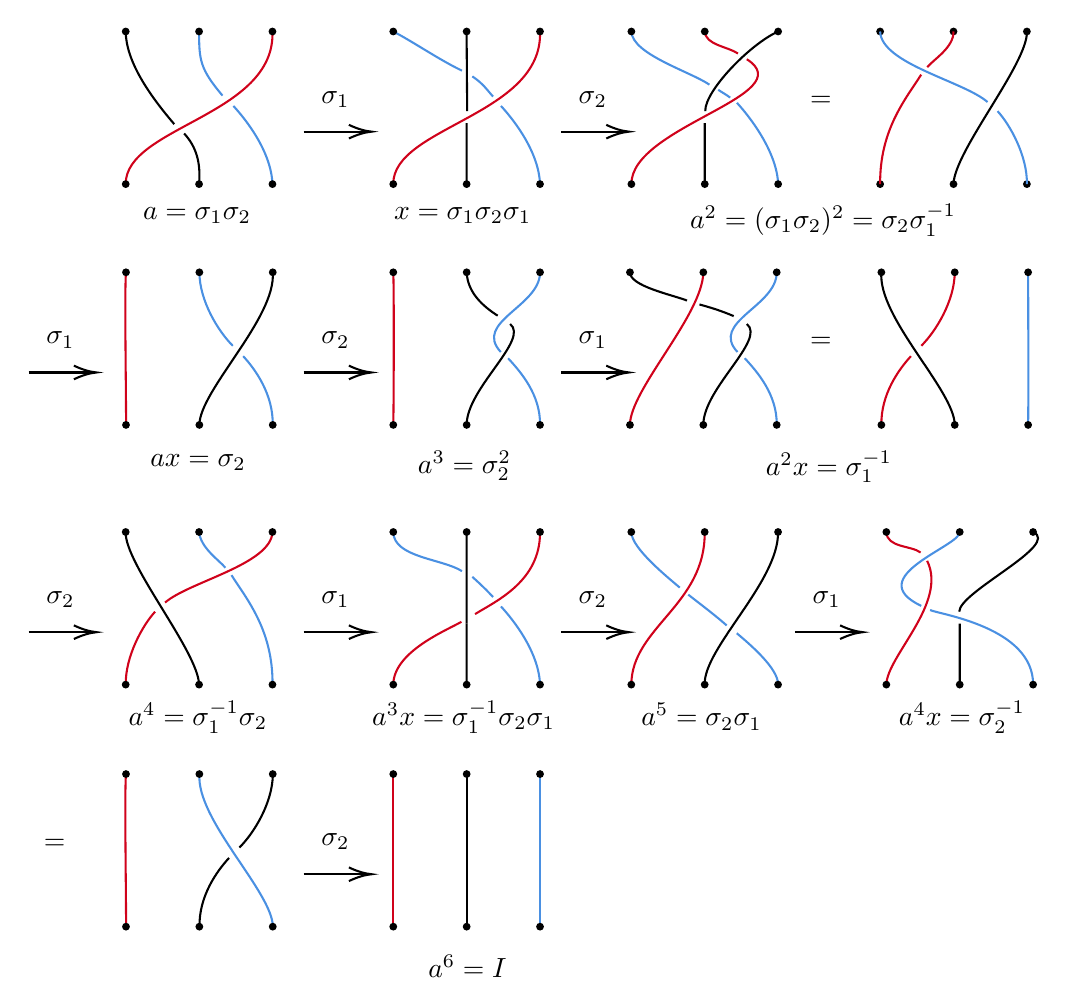
\begin{tikzpicture}[x=0.75pt,y=0.75pt,yscale=-1,xscale=1]
%uncomment if require: \path (0,465); %set diagram left start at 0, and has height of 465

%Curve Lines [id:da5252413504435514] 
\draw [color={rgb, 255:red, 74; green, 144; blue, 226 }  ,draw opacity=1 ]   (183.63,435.03) .. controls (183.52,418.41) and (146.52,383.41) .. (148.28,361.5) ;
%Curve Lines [id:da9147181023777695] 
\draw [color={rgb, 255:red, 0; green, 0; blue, 0 }  ,draw opacity=1 ]   (167.52,396.91) .. controls (174.5,389.96) and (183.52,375.41) .. (183.63,361.5) ;
%Curve Lines [id:da348533536026542] 
\draw [color={rgb, 255:red, 208; green, 2; blue, 27 }  ,draw opacity=1 ]   (112.87,435.03) .. controls (113.07,427.89) and (112.07,369.89) .. (112.87,361.5) ;
%Curve Lines [id:da6444362513322441] 
\draw [color={rgb, 255:red, 0; green, 0; blue, 0 }  ,draw opacity=1 ]   (148.28,435.03) .. controls (148.02,420.41) and (156.52,408.41) .. (162.52,401.91) ;
%Straight Lines [id:da28235646594889285] 
\draw    (112.87,361.5) ;
\draw [shift={(112.87,361.5)}, rotate = 0] [color={rgb, 255:red, 0; green, 0; blue, 0 }  ][fill={rgb, 255:red, 0; green, 0; blue, 0 }  ][line width=0.75]      (0, 0) circle [x radius= 1.34, y radius= 1.34]   ;
%Straight Lines [id:da11451267538632881] 
\draw    (148.22,361.5) ;
\draw [shift={(148.22,361.5)}, rotate = 0] [color={rgb, 255:red, 0; green, 0; blue, 0 }  ][fill={rgb, 255:red, 0; green, 0; blue, 0 }  ][line width=0.75]      (0, 0) circle [x radius= 1.34, y radius= 1.34]   ;
%Straight Lines [id:da6205259318282086] 
\draw    (183.57,361.5) ;
\draw [shift={(183.57,361.5)}, rotate = 0] [color={rgb, 255:red, 0; green, 0; blue, 0 }  ][fill={rgb, 255:red, 0; green, 0; blue, 0 }  ][line width=0.75]      (0, 0) circle [x radius= 1.34, y radius= 1.34]   ;
%Straight Lines [id:da6913883925680007] 
\draw    (112.87,435.03) ;
\draw [shift={(112.87,435.03)}, rotate = 0] [color={rgb, 255:red, 0; green, 0; blue, 0 }  ][fill={rgb, 255:red, 0; green, 0; blue, 0 }  ][line width=0.75]      (0, 0) circle [x radius= 1.34, y radius= 1.34]   ;
%Straight Lines [id:da8405933347914158] 
\draw    (148.22,435.03) ;
\draw [shift={(148.22,435.03)}, rotate = 0] [color={rgb, 255:red, 0; green, 0; blue, 0 }  ][fill={rgb, 255:red, 0; green, 0; blue, 0 }  ][line width=0.75]      (0, 0) circle [x radius= 1.34, y radius= 1.34]   ;
%Straight Lines [id:da013106392967589864] 
\draw    (183.57,435.03) ;
\draw [shift={(183.57,435.03)}, rotate = 0] [color={rgb, 255:red, 0; green, 0; blue, 0 }  ][fill={rgb, 255:red, 0; green, 0; blue, 0 }  ][line width=0.75]      (0, 0) circle [x radius= 1.34, y radius= 1.34]   ;

%Straight Lines [id:da9782562919349278] 
\draw [color={rgb, 255:red, 208; green, 2; blue, 27 }  ,draw opacity=1 ]   (241.65,361.5) -- (241.65,435.03) ;
%Straight Lines [id:da6833385473555309] 
\draw [color={rgb, 255:red, 74; green, 144; blue, 226 }  ,draw opacity=1 ]   (312.35,361.5) -- (312.35,435.03) ;
%Straight Lines [id:da5416378817329432] 
\draw    (241.65,361.5) ;
\draw [shift={(241.65,361.5)}, rotate = 0] [color={rgb, 255:red, 0; green, 0; blue, 0 }  ][fill={rgb, 255:red, 0; green, 0; blue, 0 }  ][line width=0.75]      (0, 0) circle [x radius= 1.34, y radius= 1.34]   ;
%Straight Lines [id:da7253484269458348] 
\draw    (277,361.5) ;
\draw [shift={(277,361.5)}, rotate = 0] [color={rgb, 255:red, 0; green, 0; blue, 0 }  ][fill={rgb, 255:red, 0; green, 0; blue, 0 }  ][line width=0.75]      (0, 0) circle [x radius= 1.34, y radius= 1.34]   ;
%Straight Lines [id:da772901769153256] 
\draw    (312.35,361.5) ;
\draw [shift={(312.35,361.5)}, rotate = 0] [color={rgb, 255:red, 0; green, 0; blue, 0 }  ][fill={rgb, 255:red, 0; green, 0; blue, 0 }  ][line width=0.75]      (0, 0) circle [x radius= 1.34, y radius= 1.34]   ;
%Straight Lines [id:da06299906051576465] 
\draw    (241.65,435.03) ;
\draw [shift={(241.65,435.03)}, rotate = 0] [color={rgb, 255:red, 0; green, 0; blue, 0 }  ][fill={rgb, 255:red, 0; green, 0; blue, 0 }  ][line width=0.75]      (0, 0) circle [x radius= 1.34, y radius= 1.34]   ;
%Straight Lines [id:da9993140893915438] 
\draw    (277,435.03) ;
\draw [shift={(277,435.03)}, rotate = 0] [color={rgb, 255:red, 0; green, 0; blue, 0 }  ][fill={rgb, 255:red, 0; green, 0; blue, 0 }  ][line width=0.75]      (0, 0) circle [x radius= 1.34, y radius= 1.34]   ;
%Straight Lines [id:da11024546054753626] 
\draw    (312.35,435.03) ;
\draw [shift={(312.35,435.03)}, rotate = 0] [color={rgb, 255:red, 0; green, 0; blue, 0 }  ][fill={rgb, 255:red, 0; green, 0; blue, 0 }  ][line width=0.75]      (0, 0) circle [x radius= 1.34, y radius= 1.34]   ;
%Straight Lines [id:da8503600630706685] 
\draw    (277,361.5) -- (277,435.03) ;

%Curve Lines [id:da9317966994630702] 
\draw [color={rgb, 255:red, 208; green, 2; blue, 27 }  ,draw opacity=1 ]   (241.65,318.41) .. controls (241.74,302.49) and (267.61,292.15) .. (274.47,288.15) ;
%Curve Lines [id:da5877737916220236] 
\draw [color={rgb, 255:red, 208; green, 2; blue, 27 }  ,draw opacity=1 ]   (281.04,284.43) .. controls (291.47,278) and (312.54,268.49) .. (312.35,244.88) ;
%Curve Lines [id:da5194005947655427] 
\draw [color={rgb, 255:red, 74; green, 144; blue, 226 }  ,draw opacity=1 ]   (274.74,263.74) .. controls (265.32,257.73) and (241.82,257.23) .. (241.65,244.88) ;
%Curve Lines [id:da8198853449051793] 
\draw [color={rgb, 255:red, 74; green, 144; blue, 226 }  ,draw opacity=1 ]   (312.35,318.41) .. controls (311.79,302.76) and (299.54,287.26) .. (293.54,280.76) ;
%Straight Lines [id:da17644852037663972] 
\draw    (241.65,244.88) ;
\draw [shift={(241.65,244.88)}, rotate = 0] [color={rgb, 255:red, 0; green, 0; blue, 0 }  ][fill={rgb, 255:red, 0; green, 0; blue, 0 }  ][line width=0.75]      (0, 0) circle [x radius= 1.34, y radius= 1.34]   ;
%Straight Lines [id:da8927646988377032] 
\draw    (277,244.88) ;
\draw [shift={(277,244.88)}, rotate = 0] [color={rgb, 255:red, 0; green, 0; blue, 0 }  ][fill={rgb, 255:red, 0; green, 0; blue, 0 }  ][line width=0.75]      (0, 0) circle [x radius= 1.34, y radius= 1.34]   ;
%Straight Lines [id:da7172914138201123] 
\draw    (312.35,244.88) ;
\draw [shift={(312.35,244.88)}, rotate = 0] [color={rgb, 255:red, 0; green, 0; blue, 0 }  ][fill={rgb, 255:red, 0; green, 0; blue, 0 }  ][line width=0.75]      (0, 0) circle [x radius= 1.34, y radius= 1.34]   ;
%Straight Lines [id:da4481635250097269] 
\draw    (241.65,318.41) ;
\draw [shift={(241.65,318.41)}, rotate = 0] [color={rgb, 255:red, 0; green, 0; blue, 0 }  ][fill={rgb, 255:red, 0; green, 0; blue, 0 }  ][line width=0.75]      (0, 0) circle [x radius= 1.34, y radius= 1.34]   ;
%Straight Lines [id:da4835384780671981] 
\draw    (277,318.41) ;
\draw [shift={(277,318.41)}, rotate = 0] [color={rgb, 255:red, 0; green, 0; blue, 0 }  ][fill={rgb, 255:red, 0; green, 0; blue, 0 }  ][line width=0.75]      (0, 0) circle [x radius= 1.34, y radius= 1.34]   ;
%Straight Lines [id:da07018173882647472] 
\draw    (312.35,318.41) ;
\draw [shift={(312.35,318.41)}, rotate = 0] [color={rgb, 255:red, 0; green, 0; blue, 0 }  ][fill={rgb, 255:red, 0; green, 0; blue, 0 }  ][line width=0.75]      (0, 0) circle [x radius= 1.34, y radius= 1.34]   ;
%Curve Lines [id:da13368884102800926] 
\draw [color={rgb, 255:red, 0; green, 0; blue, 0 }  ,draw opacity=1 ]   (277,318.41) .. controls (276.99,311.49) and (276.98,294.85) .. (276.99,288.99) ;
%Curve Lines [id:da10360528961604909] 
\draw [color={rgb, 255:red, 0; green, 0; blue, 0 }  ,draw opacity=1 ]   (276.99,288.99) .. controls (276.98,282.07) and (276.99,250.74) .. (277,244.88) ;
%Curve Lines [id:da8258348609478736] 
\draw [color={rgb, 255:red, 74; green, 144; blue, 226 }  ,draw opacity=1 ]   (289.74,276.24) .. controls (286.74,272.99) and (283.74,270.09) .. (279.74,266.49) ;

%Curve Lines [id:da3922843167953176] 
\draw [color={rgb, 255:red, 74; green, 144; blue, 226 }  ,draw opacity=1 ]   (379.67,271.67) .. controls (374.29,267.04) and (356.29,252.67) .. (356.33,244.88) ;
%Curve Lines [id:da07617514101534506] 
\draw [color={rgb, 255:red, 74; green, 144; blue, 226 }  ,draw opacity=1 ]   (427.03,318.41) .. controls (427.27,310.54) and (412.77,298.41) .. (407.14,293.66) ;
%Curve Lines [id:da1673996882564608] 
\draw [color={rgb, 255:red, 208; green, 2; blue, 27 }  ,draw opacity=1 ]   (356.33,318.41) .. controls (356.54,290.67) and (392.08,280.17) .. (391.68,244.88) ;
%Straight Lines [id:da06734218094749522] 
\draw    (356.33,244.88) ;
\draw [shift={(356.33,244.88)}, rotate = 0] [color={rgb, 255:red, 0; green, 0; blue, 0 }  ][fill={rgb, 255:red, 0; green, 0; blue, 0 }  ][line width=0.75]      (0, 0) circle [x radius= 1.34, y radius= 1.34]   ;
%Straight Lines [id:da6694734769505588] 
\draw    (391.68,244.88) ;
\draw [shift={(391.68,244.88)}, rotate = 0] [color={rgb, 255:red, 0; green, 0; blue, 0 }  ][fill={rgb, 255:red, 0; green, 0; blue, 0 }  ][line width=0.75]      (0, 0) circle [x radius= 1.34, y radius= 1.34]   ;
%Straight Lines [id:da5856086237870681] 
\draw    (427.03,244.88) ;
\draw [shift={(427.03,244.88)}, rotate = 0] [color={rgb, 255:red, 0; green, 0; blue, 0 }  ][fill={rgb, 255:red, 0; green, 0; blue, 0 }  ][line width=0.75]      (0, 0) circle [x radius= 1.34, y radius= 1.34]   ;
%Straight Lines [id:da9509010081652569] 
\draw    (356.33,318.41) ;
\draw [shift={(356.33,318.41)}, rotate = 0] [color={rgb, 255:red, 0; green, 0; blue, 0 }  ][fill={rgb, 255:red, 0; green, 0; blue, 0 }  ][line width=0.75]      (0, 0) circle [x radius= 1.34, y radius= 1.34]   ;
%Straight Lines [id:da3662259854691199] 
\draw    (391.68,318.41) ;
\draw [shift={(391.68,318.41)}, rotate = 0] [color={rgb, 255:red, 0; green, 0; blue, 0 }  ][fill={rgb, 255:red, 0; green, 0; blue, 0 }  ][line width=0.75]      (0, 0) circle [x radius= 1.34, y radius= 1.34]   ;
%Straight Lines [id:da2054126980865021] 
\draw    (427.03,318.41) ;
\draw [shift={(427.03,318.41)}, rotate = 0] [color={rgb, 255:red, 0; green, 0; blue, 0 }  ][fill={rgb, 255:red, 0; green, 0; blue, 0 }  ][line width=0.75]      (0, 0) circle [x radius= 1.34, y radius= 1.34]   ;
%Curve Lines [id:da29431690371256725] 
\draw [color={rgb, 255:red, 0; green, 0; blue, 0 }  ,draw opacity=1 ]   (391.68,318.41) .. controls (391.08,300.83) and (427.41,268.83) .. (427.03,244.88) ;
%Curve Lines [id:da04036551229532681] 
\draw [color={rgb, 255:red, 74; green, 144; blue, 226 }  ,draw opacity=1 ]   (402.28,289.91) .. controls (396.65,284.91) and (389.15,279.29) .. (383.77,275.07) ;

%Curve Lines [id:da12144365042238969] 
\draw [color={rgb, 255:red, 208; green, 2; blue, 27 }  ,draw opacity=1 ]   (131.69,278.88) .. controls (143.12,268.88) and (182.89,260.48) .. (183.43,244.88) ;
%Curve Lines [id:da8412767835327639] 
\draw [color={rgb, 255:red, 74; green, 144; blue, 226 }  ,draw opacity=1 ]   (160.74,262.07) .. controls (157.29,258.08) and (148.85,252.48) .. (148.08,244.88) ;
%Curve Lines [id:da9122507729373719] 
\draw [color={rgb, 255:red, 208; green, 2; blue, 27 }  ,draw opacity=1 ]   (112.76,318.41) .. controls (112.49,304.88) and (120.89,289.78) .. (126.89,283.28) ;
%Curve Lines [id:da5633782962927263] 
\draw [color={rgb, 255:red, 74; green, 144; blue, 226 }  ,draw opacity=1 ]   (183.47,318.41) .. controls (183.69,292.48) and (171.41,277.68) .. (163.69,265.68) ;
%Straight Lines [id:da10792379177305467] 
\draw    (112.72,244.88) ;
\draw [shift={(112.72,244.88)}, rotate = 0] [color={rgb, 255:red, 0; green, 0; blue, 0 }  ][fill={rgb, 255:red, 0; green, 0; blue, 0 }  ][line width=0.75]      (0, 0) circle [x radius= 1.34, y radius= 1.34]   ;
%Straight Lines [id:da010060016550406559] 
\draw    (148.08,244.88) ;
\draw [shift={(148.08,244.88)}, rotate = 0] [color={rgb, 255:red, 0; green, 0; blue, 0 }  ][fill={rgb, 255:red, 0; green, 0; blue, 0 }  ][line width=0.75]      (0, 0) circle [x radius= 1.34, y radius= 1.34]   ;
%Straight Lines [id:da8292875054749858] 
\draw    (183.43,244.88) ;
\draw [shift={(183.43,244.88)}, rotate = 0] [color={rgb, 255:red, 0; green, 0; blue, 0 }  ][fill={rgb, 255:red, 0; green, 0; blue, 0 }  ][line width=0.75]      (0, 0) circle [x radius= 1.34, y radius= 1.34]   ;
%Straight Lines [id:da26463074487737237] 
\draw    (112.72,318.41) ;
\draw [shift={(112.72,318.41)}, rotate = 0] [color={rgb, 255:red, 0; green, 0; blue, 0 }  ][fill={rgb, 255:red, 0; green, 0; blue, 0 }  ][line width=0.75]      (0, 0) circle [x radius= 1.34, y radius= 1.34]   ;
%Straight Lines [id:da4308612317515259] 
\draw    (148.08,318.41) ;
\draw [shift={(148.08,318.41)}, rotate = 0] [color={rgb, 255:red, 0; green, 0; blue, 0 }  ][fill={rgb, 255:red, 0; green, 0; blue, 0 }  ][line width=0.75]      (0, 0) circle [x radius= 1.34, y radius= 1.34]   ;
%Straight Lines [id:da7552639155962018] 
\draw    (183.43,318.41) ;
\draw [shift={(183.43,318.41)}, rotate = 0] [color={rgb, 255:red, 0; green, 0; blue, 0 }  ][fill={rgb, 255:red, 0; green, 0; blue, 0 }  ][line width=0.75]      (0, 0) circle [x radius= 1.34, y radius= 1.34]   ;
%Curve Lines [id:da3334764215595696] 
\draw [color={rgb, 255:red, 0; green, 0; blue, 0 }  ,draw opacity=1 ]   (148.08,318.41) .. controls (147.69,302.48) and (112.09,260.08) .. (112.72,244.88) ;

%Curve Lines [id:da2145063670812013] 
\draw [color={rgb, 255:red, 208; green, 2; blue, 27 }  ,draw opacity=1 ]   (495.72,254.76) .. controls (491.14,251.33) and (479.43,252.47) .. (479.21,244.88) ;
%Curve Lines [id:da6535311024967561] 
\draw [color={rgb, 255:red, 74; green, 144; blue, 226 }  ,draw opacity=1 ]   (496,280.47) .. controls (466.57,266.47) and (515.14,251.61) .. (514.56,244.88) ;
%Curve Lines [id:da2779400155475893] 
\draw [color={rgb, 255:red, 208; green, 2; blue, 27 }  ,draw opacity=1 ]   (479.21,318.41) .. controls (479.43,304.76) and (508.86,279.04) .. (498.86,258.76) ;
%Curve Lines [id:da6336705993500078] 
\draw [color={rgb, 255:red, 74; green, 144; blue, 226 }  ,draw opacity=1 ]   (549.91,318.41) .. controls (550.11,290.67) and (504.29,284.47) .. (500.29,282.47) ;
%Straight Lines [id:da7662867462277332] 
\draw    (479.21,244.88) ;
\draw [shift={(479.21,244.88)}, rotate = 0] [color={rgb, 255:red, 0; green, 0; blue, 0 }  ][fill={rgb, 255:red, 0; green, 0; blue, 0 }  ][line width=0.75]      (0, 0) circle [x radius= 1.34, y radius= 1.34]   ;
%Straight Lines [id:da9222722696310435] 
\draw    (514.56,244.88) ;
\draw [shift={(514.56,244.88)}, rotate = 0] [color={rgb, 255:red, 0; green, 0; blue, 0 }  ][fill={rgb, 255:red, 0; green, 0; blue, 0 }  ][line width=0.75]      (0, 0) circle [x radius= 1.34, y radius= 1.34]   ;
%Straight Lines [id:da16949486887693466] 
\draw    (549.91,244.88) ;
\draw [shift={(549.91,244.88)}, rotate = 0] [color={rgb, 255:red, 0; green, 0; blue, 0 }  ][fill={rgb, 255:red, 0; green, 0; blue, 0 }  ][line width=0.75]      (0, 0) circle [x radius= 1.34, y radius= 1.34]   ;
%Straight Lines [id:da9490828763400059] 
\draw    (479.21,318.41) ;
\draw [shift={(479.21,318.41)}, rotate = 0] [color={rgb, 255:red, 0; green, 0; blue, 0 }  ][fill={rgb, 255:red, 0; green, 0; blue, 0 }  ][line width=0.75]      (0, 0) circle [x radius= 1.34, y radius= 1.34]   ;
%Straight Lines [id:da8568155778542959] 
\draw    (514.56,318.41) ;
\draw [shift={(514.56,318.41)}, rotate = 0] [color={rgb, 255:red, 0; green, 0; blue, 0 }  ][fill={rgb, 255:red, 0; green, 0; blue, 0 }  ][line width=0.75]      (0, 0) circle [x radius= 1.34, y radius= 1.34]   ;
%Straight Lines [id:da9702244781945606] 
\draw    (549.91,318.41) ;
\draw [shift={(549.91,318.41)}, rotate = 0] [color={rgb, 255:red, 0; green, 0; blue, 0 }  ][fill={rgb, 255:red, 0; green, 0; blue, 0 }  ][line width=0.75]      (0, 0) circle [x radius= 1.34, y radius= 1.34]   ;
%Curve Lines [id:da43322352220872484] 
\draw [color={rgb, 255:red, 0; green, 0; blue, 0 }  ,draw opacity=1 ]   (514.56,318.41) .. controls (514.56,311.49) and (514.57,294.85) .. (514.56,288.99) ;
%Curve Lines [id:da6895880876391953] 
\draw [color={rgb, 255:red, 0; green, 0; blue, 0 }  ,draw opacity=1 ]   (514.31,283.24) .. controls (514.56,273.49) and (563.51,250.99) .. (549.91,244.88) ;

%Curve Lines [id:da424096886489588] 
\draw [color={rgb, 255:red, 208; green, 2; blue, 27 }  ,draw opacity=1 ]   (496.05,155.17) .. controls (503.02,148.22) and (512.05,133.67) .. (512.16,119.76) ;
%Curve Lines [id:da9735521729841601] 
\draw [color={rgb, 255:red, 208; green, 2; blue, 27 }  ,draw opacity=1 ]   (476.81,193.29) .. controls (476.55,178.67) and (485.05,166.67) .. (491.05,160.17) ;
%Curve Lines [id:da7877183389146603] 
\draw [color={rgb, 255:red, 74; green, 144; blue, 226 }  ,draw opacity=1 ]   (547.51,193.29) .. controls (547.71,186.14) and (547.56,128.93) .. (547.51,119.76) ;
%Straight Lines [id:da36626916256243924] 
\draw    (476.81,119.76) ;
\draw [shift={(476.81,119.76)}, rotate = 0] [color={rgb, 255:red, 0; green, 0; blue, 0 }  ][fill={rgb, 255:red, 0; green, 0; blue, 0 }  ][line width=0.75]      (0, 0) circle [x radius= 1.34, y radius= 1.34]   ;
%Straight Lines [id:da912716328056751] 
\draw    (512.16,119.76) ;
\draw [shift={(512.16,119.76)}, rotate = 0] [color={rgb, 255:red, 0; green, 0; blue, 0 }  ][fill={rgb, 255:red, 0; green, 0; blue, 0 }  ][line width=0.75]      (0, 0) circle [x radius= 1.34, y radius= 1.34]   ;
%Straight Lines [id:da23104269022918222] 
\draw    (547.51,119.76) ;
\draw [shift={(547.51,119.76)}, rotate = 0] [color={rgb, 255:red, 0; green, 0; blue, 0 }  ][fill={rgb, 255:red, 0; green, 0; blue, 0 }  ][line width=0.75]      (0, 0) circle [x radius= 1.34, y radius= 1.34]   ;
%Straight Lines [id:da7863930593361814] 
\draw    (476.81,193.29) ;
\draw [shift={(476.81,193.29)}, rotate = 0] [color={rgb, 255:red, 0; green, 0; blue, 0 }  ][fill={rgb, 255:red, 0; green, 0; blue, 0 }  ][line width=0.75]      (0, 0) circle [x radius= 1.34, y radius= 1.34]   ;
%Straight Lines [id:da954584959041797] 
\draw    (512.16,193.29) ;
\draw [shift={(512.16,193.29)}, rotate = 0] [color={rgb, 255:red, 0; green, 0; blue, 0 }  ][fill={rgb, 255:red, 0; green, 0; blue, 0 }  ][line width=0.75]      (0, 0) circle [x radius= 1.34, y radius= 1.34]   ;
%Straight Lines [id:da9455082188404524] 
\draw    (547.51,193.29) ;
\draw [shift={(547.51,193.29)}, rotate = 0] [color={rgb, 255:red, 0; green, 0; blue, 0 }  ][fill={rgb, 255:red, 0; green, 0; blue, 0 }  ][line width=0.75]      (0, 0) circle [x radius= 1.34, y radius= 1.34]   ;
%Curve Lines [id:da03405643202963371] 
\draw [color={rgb, 255:red, 0; green, 0; blue, 0 }  ,draw opacity=1 ]   (512.16,193.29) .. controls (512.05,176.67) and (475.05,141.67) .. (476.81,119.76) ;

%Curve Lines [id:da08845531509426086] 
\draw [color={rgb, 255:red, 74; green, 144; blue, 226 }  ,draw opacity=1 ]   (407.48,158.17) .. controls (393.98,143.67) and (426.48,136.17) .. (426.38,119.76) ;
%Curve Lines [id:da5558602744380698] 
\draw [color={rgb, 255:red, 208; green, 2; blue, 27 }  ,draw opacity=1 ]   (355.68,193.29) .. controls (355.66,176.36) and (390.66,140.36) .. (391.03,119.76) ;
%Curve Lines [id:da15388414242878756] 
\draw [color={rgb, 255:red, 74; green, 144; blue, 226 }  ,draw opacity=1 ]   (426.38,193.29) .. controls (426.64,178.67) and (416.98,167.67) .. (410.98,161.17) ;
%Straight Lines [id:da5524321963390426] 
\draw    (355.68,119.76) ;
\draw [shift={(355.68,119.76)}, rotate = 0] [color={rgb, 255:red, 0; green, 0; blue, 0 }  ][fill={rgb, 255:red, 0; green, 0; blue, 0 }  ][line width=0.75]      (0, 0) circle [x radius= 1.34, y radius= 1.34]   ;
%Straight Lines [id:da12912732876231559] 
\draw    (391.03,119.76) ;
\draw [shift={(391.03,119.76)}, rotate = 0] [color={rgb, 255:red, 0; green, 0; blue, 0 }  ][fill={rgb, 255:red, 0; green, 0; blue, 0 }  ][line width=0.75]      (0, 0) circle [x radius= 1.34, y radius= 1.34]   ;
%Straight Lines [id:da5634141249355558] 
\draw    (426.38,119.76) ;
\draw [shift={(426.38,119.76)}, rotate = 0] [color={rgb, 255:red, 0; green, 0; blue, 0 }  ][fill={rgb, 255:red, 0; green, 0; blue, 0 }  ][line width=0.75]      (0, 0) circle [x radius= 1.34, y radius= 1.34]   ;
%Straight Lines [id:da8463457122558182] 
\draw    (355.68,193.29) ;
\draw [shift={(355.68,193.29)}, rotate = 0] [color={rgb, 255:red, 0; green, 0; blue, 0 }  ][fill={rgb, 255:red, 0; green, 0; blue, 0 }  ][line width=0.75]      (0, 0) circle [x radius= 1.34, y radius= 1.34]   ;
%Straight Lines [id:da28455770029011385] 
\draw    (391.03,193.29) ;
\draw [shift={(391.03,193.29)}, rotate = 0] [color={rgb, 255:red, 0; green, 0; blue, 0 }  ][fill={rgb, 255:red, 0; green, 0; blue, 0 }  ][line width=0.75]      (0, 0) circle [x radius= 1.34, y radius= 1.34]   ;
%Straight Lines [id:da4885284813983697] 
\draw    (426.38,193.29) ;
\draw [shift={(426.38,193.29)}, rotate = 0] [color={rgb, 255:red, 0; green, 0; blue, 0 }  ][fill={rgb, 255:red, 0; green, 0; blue, 0 }  ][line width=0.75]      (0, 0) circle [x radius= 1.34, y radius= 1.34]   ;
%Curve Lines [id:da31123488880616756] 
\draw [color={rgb, 255:red, 0; green, 0; blue, 0 }  ,draw opacity=1 ]   (391.03,193.29) .. controls (390.98,175.67) and (421.48,152.17) .. (411.98,144.67) ;
%Curve Lines [id:da4722994912110816] 
\draw [color={rgb, 255:red, 0; green, 0; blue, 0 }  ,draw opacity=1 ]   (383.16,133.36) .. controls (375.16,130.36) and (355.66,126.36) .. (355.68,119.76) ;
%Curve Lines [id:da19956469737235105] 
\draw [color={rgb, 255:red, 0; green, 0; blue, 0 }  ,draw opacity=1 ]   (405.66,140.86) .. controls (400.11,138.52) and (395.61,137.01) .. (389.18,135.26) ;


%Curve Lines [id:da14378438043592778] 
\draw [color={rgb, 255:red, 74; green, 144; blue, 226 }  ,draw opacity=1 ]   (164.33,155.17) .. controls (157.35,148.22) and (148.33,133.67) .. (148.22,119.76) ;
%Curve Lines [id:da9437693719694413] 
\draw [color={rgb, 255:red, 208; green, 2; blue, 27 }  ,draw opacity=1 ]   (112.87,193.29) .. controls (113.07,186.14) and (112.07,128.14) .. (112.87,119.76) ;
%Curve Lines [id:da6341367322082865] 
\draw [color={rgb, 255:red, 74; green, 144; blue, 226 }  ,draw opacity=1 ]   (183.57,193.29) .. controls (183.83,178.67) and (175.33,166.67) .. (169.33,160.17) ;
%Straight Lines [id:da8805900451887314] 
\draw    (112.87,119.76) ;
\draw [shift={(112.87,119.76)}, rotate = 0] [color={rgb, 255:red, 0; green, 0; blue, 0 }  ][fill={rgb, 255:red, 0; green, 0; blue, 0 }  ][line width=0.75]      (0, 0) circle [x radius= 1.34, y radius= 1.34]   ;
%Straight Lines [id:da9748749410097683] 
\draw    (148.22,119.76) ;
\draw [shift={(148.22,119.76)}, rotate = 0] [color={rgb, 255:red, 0; green, 0; blue, 0 }  ][fill={rgb, 255:red, 0; green, 0; blue, 0 }  ][line width=0.75]      (0, 0) circle [x radius= 1.34, y radius= 1.34]   ;
%Straight Lines [id:da7196347270051509] 
\draw    (183.57,119.76) ;
\draw [shift={(183.57,119.76)}, rotate = 0] [color={rgb, 255:red, 0; green, 0; blue, 0 }  ][fill={rgb, 255:red, 0; green, 0; blue, 0 }  ][line width=0.75]      (0, 0) circle [x radius= 1.34, y radius= 1.34]   ;
%Straight Lines [id:da3985775893699106] 
\draw    (112.87,193.29) ;
\draw [shift={(112.87,193.29)}, rotate = 0] [color={rgb, 255:red, 0; green, 0; blue, 0 }  ][fill={rgb, 255:red, 0; green, 0; blue, 0 }  ][line width=0.75]      (0, 0) circle [x radius= 1.34, y radius= 1.34]   ;
%Straight Lines [id:da09238097518207833] 
\draw    (148.22,193.29) ;
\draw [shift={(148.22,193.29)}, rotate = 0] [color={rgb, 255:red, 0; green, 0; blue, 0 }  ][fill={rgb, 255:red, 0; green, 0; blue, 0 }  ][line width=0.75]      (0, 0) circle [x radius= 1.34, y radius= 1.34]   ;
%Straight Lines [id:da7677605995643573] 
\draw    (183.57,193.29) ;
\draw [shift={(183.57,193.29)}, rotate = 0] [color={rgb, 255:red, 0; green, 0; blue, 0 }  ][fill={rgb, 255:red, 0; green, 0; blue, 0 }  ][line width=0.75]      (0, 0) circle [x radius= 1.34, y radius= 1.34]   ;
%Curve Lines [id:da01388428389362395] 
\draw [color={rgb, 255:red, 0; green, 0; blue, 0 }  ,draw opacity=1 ]   (148.22,193.29) .. controls (148.33,176.67) and (185.33,141.67) .. (183.57,119.76) ;

%Curve Lines [id:da4578655914367271] 
\draw [color={rgb, 255:red, 74; green, 144; blue, 226 }  ,draw opacity=1 ]   (293.45,158.17) .. controls (279.95,143.67) and (312.45,136.17) .. (312.35,119.76) ;
%Curve Lines [id:da5301851342044788] 
\draw [color={rgb, 255:red, 208; green, 2; blue, 27 }  ,draw opacity=1 ]   (241.65,193.29) .. controls (241.85,186.14) and (242.06,130.03) .. (241.65,119.76) ;
%Curve Lines [id:da7500130173506847] 
\draw [color={rgb, 255:red, 74; green, 144; blue, 226 }  ,draw opacity=1 ]   (312.35,193.29) .. controls (312.61,178.67) and (302.95,167.67) .. (296.95,161.17) ;
%Straight Lines [id:da7071615395585049] 
\draw    (241.65,119.76) ;
\draw [shift={(241.65,119.76)}, rotate = 0] [color={rgb, 255:red, 0; green, 0; blue, 0 }  ][fill={rgb, 255:red, 0; green, 0; blue, 0 }  ][line width=0.75]      (0, 0) circle [x radius= 1.34, y radius= 1.34]   ;
%Straight Lines [id:da12419967854638947] 
\draw    (277,119.76) ;
\draw [shift={(277,119.76)}, rotate = 0] [color={rgb, 255:red, 0; green, 0; blue, 0 }  ][fill={rgb, 255:red, 0; green, 0; blue, 0 }  ][line width=0.75]      (0, 0) circle [x radius= 1.34, y radius= 1.34]   ;
%Straight Lines [id:da0669035594397025] 
\draw    (312.35,119.76) ;
\draw [shift={(312.35,119.76)}, rotate = 0] [color={rgb, 255:red, 0; green, 0; blue, 0 }  ][fill={rgb, 255:red, 0; green, 0; blue, 0 }  ][line width=0.75]      (0, 0) circle [x radius= 1.34, y radius= 1.34]   ;
%Straight Lines [id:da05634450937126312] 
\draw    (241.65,193.29) ;
\draw [shift={(241.65,193.29)}, rotate = 0] [color={rgb, 255:red, 0; green, 0; blue, 0 }  ][fill={rgb, 255:red, 0; green, 0; blue, 0 }  ][line width=0.75]      (0, 0) circle [x radius= 1.34, y radius= 1.34]   ;
%Straight Lines [id:da39635687797934427] 
\draw    (277,193.29) ;
\draw [shift={(277,193.29)}, rotate = 0] [color={rgb, 255:red, 0; green, 0; blue, 0 }  ][fill={rgb, 255:red, 0; green, 0; blue, 0 }  ][line width=0.75]      (0, 0) circle [x radius= 1.34, y radius= 1.34]   ;
%Straight Lines [id:da8534091344955357] 
\draw    (312.35,193.29) ;
\draw [shift={(312.35,193.29)}, rotate = 0] [color={rgb, 255:red, 0; green, 0; blue, 0 }  ][fill={rgb, 255:red, 0; green, 0; blue, 0 }  ][line width=0.75]      (0, 0) circle [x radius= 1.34, y radius= 1.34]   ;
%Curve Lines [id:da011402099345569239] 
\draw [color={rgb, 255:red, 0; green, 0; blue, 0 }  ,draw opacity=1 ]   (277,193.29) .. controls (276.95,175.67) and (307.45,152.17) .. (297.95,144.67) ;
%Curve Lines [id:da7316918837650417] 
\draw [color={rgb, 255:red, 0; green, 0; blue, 0 }  ,draw opacity=1 ]   (291.95,140.67) .. controls (284.95,136.17) and (277.45,129.67) .. (277,119.76) ;

%Curve Lines [id:da5580708873603075] 
\draw [color={rgb, 255:red, 74; green, 144; blue, 226 }  ,draw opacity=1 ]   (274.73,22.6) .. controls (263.73,17.35) and (251.48,8.85) .. (241.64,3.74) ;
%Curve Lines [id:da574513066926746] 
\draw [color={rgb, 255:red, 74; green, 144; blue, 226 }  ,draw opacity=1 ]   (312.34,77.27) .. controls (311.78,61.62) and (299.53,46.12) .. (293.53,39.62) ;
%Curve Lines [id:da8200994488960685] 
\draw [color={rgb, 255:red, 208; green, 2; blue, 27 }  ,draw opacity=1 ]   (241.64,77.27) .. controls (241.43,49.53) and (313.83,44.33) .. (312.34,3.74) ;
%Straight Lines [id:da05840758051395456] 
\draw    (241.64,3.74) ;
\draw [shift={(241.64,3.74)}, rotate = 0] [color={rgb, 255:red, 0; green, 0; blue, 0 }  ][fill={rgb, 255:red, 0; green, 0; blue, 0 }  ][line width=0.75]      (0, 0) circle [x radius= 1.34, y radius= 1.34]   ;
%Straight Lines [id:da3401972689143915] 
\draw    (276.99,3.74) ;
\draw [shift={(276.99,3.74)}, rotate = 0] [color={rgb, 255:red, 0; green, 0; blue, 0 }  ][fill={rgb, 255:red, 0; green, 0; blue, 0 }  ][line width=0.75]      (0, 0) circle [x radius= 1.34, y radius= 1.34]   ;
%Straight Lines [id:da6610618759288125] 
\draw    (312.34,3.74) ;
\draw [shift={(312.34,3.74)}, rotate = 0] [color={rgb, 255:red, 0; green, 0; blue, 0 }  ][fill={rgb, 255:red, 0; green, 0; blue, 0 }  ][line width=0.75]      (0, 0) circle [x radius= 1.34, y radius= 1.34]   ;
%Straight Lines [id:da6996997954330149] 
\draw    (241.64,77.27) ;
\draw [shift={(241.64,77.27)}, rotate = 0] [color={rgb, 255:red, 0; green, 0; blue, 0 }  ][fill={rgb, 255:red, 0; green, 0; blue, 0 }  ][line width=0.75]      (0, 0) circle [x radius= 1.34, y radius= 1.34]   ;
%Straight Lines [id:da07499564117137192] 
\draw    (276.99,77.27) ;
\draw [shift={(276.99,77.27)}, rotate = 0] [color={rgb, 255:red, 0; green, 0; blue, 0 }  ][fill={rgb, 255:red, 0; green, 0; blue, 0 }  ][line width=0.75]      (0, 0) circle [x radius= 1.34, y radius= 1.34]   ;
%Straight Lines [id:da5596153957008649] 
\draw    (312.34,77.27) ;
\draw [shift={(312.34,77.27)}, rotate = 0] [color={rgb, 255:red, 0; green, 0; blue, 0 }  ][fill={rgb, 255:red, 0; green, 0; blue, 0 }  ][line width=0.75]      (0, 0) circle [x radius= 1.34, y radius= 1.34]   ;
%Curve Lines [id:da35438034254363404] 
\draw [color={rgb, 255:red, 0; green, 0; blue, 0 }  ,draw opacity=1 ]   (276.99,77.27) .. controls (276.98,70.35) and (276.97,53.71) .. (276.98,47.85) ;
%Curve Lines [id:da37954887226834666] 
\draw [color={rgb, 255:red, 0; green, 0; blue, 0 }  ,draw opacity=1 ]   (277.23,42.1) .. controls (277.22,35.18) and (276.98,9.6) .. (276.99,3.74) ;
%Curve Lines [id:da09241809520265609] 
\draw [color={rgb, 255:red, 74; green, 144; blue, 226 }  ,draw opacity=1 ]   (289.73,35.1) .. controls (286.73,31.85) and (285.23,29.1) .. (279.73,25.35) ;

%Curve Lines [id:da9181390015334914] 
\draw [color={rgb, 255:red, 74; green, 144; blue, 226 }  ,draw opacity=1 ]   (393.97,29.35) .. controls (384.22,22.85) and (356.74,14.68) .. (356.37,3.74) ;
%Curve Lines [id:da058417116418309156] 
\draw [color={rgb, 255:red, 208; green, 2; blue, 27 }  ,draw opacity=1 ]   (407.72,14.35) .. controls (402.47,10.85) and (392.22,10.35) .. (391.72,3.74) ;
%Curve Lines [id:da9655248014379656] 
\draw [color={rgb, 255:red, 74; green, 144; blue, 226 }  ,draw opacity=1 ]   (427.07,77.27) .. controls (426.51,61.62) and (413.22,44.6) .. (407.22,38.1) ;
%Curve Lines [id:da14956115166036343] 
\draw [color={rgb, 255:red, 208; green, 2; blue, 27 }  ,draw opacity=1 ]   (356.37,77.27) .. controls (356.16,49.53) and (438.97,34.35) .. (411.97,17.1) ;
%Straight Lines [id:da668236789506365] 
\draw    (356.37,3.74) ;
\draw [shift={(356.37,3.74)}, rotate = 0] [color={rgb, 255:red, 0; green, 0; blue, 0 }  ][fill={rgb, 255:red, 0; green, 0; blue, 0 }  ][line width=0.75]      (0, 0) circle [x radius= 1.34, y radius= 1.34]   ;
%Straight Lines [id:da7785203801857488] 
\draw    (391.72,3.74) ;
\draw [shift={(391.72,3.74)}, rotate = 0] [color={rgb, 255:red, 0; green, 0; blue, 0 }  ][fill={rgb, 255:red, 0; green, 0; blue, 0 }  ][line width=0.75]      (0, 0) circle [x radius= 1.34, y radius= 1.34]   ;
%Straight Lines [id:da20790616860526812] 
\draw    (427.07,3.74) ;
\draw [shift={(427.07,3.74)}, rotate = 0] [color={rgb, 255:red, 0; green, 0; blue, 0 }  ][fill={rgb, 255:red, 0; green, 0; blue, 0 }  ][line width=0.75]      (0, 0) circle [x radius= 1.34, y radius= 1.34]   ;
%Straight Lines [id:da9261107590894764] 
\draw    (356.37,77.27) ;
\draw [shift={(356.37,77.27)}, rotate = 0] [color={rgb, 255:red, 0; green, 0; blue, 0 }  ][fill={rgb, 255:red, 0; green, 0; blue, 0 }  ][line width=0.75]      (0, 0) circle [x radius= 1.34, y radius= 1.34]   ;
%Straight Lines [id:da8501051671571291] 
\draw    (391.72,77.27) ;
\draw [shift={(391.72,77.27)}, rotate = 0] [color={rgb, 255:red, 0; green, 0; blue, 0 }  ][fill={rgb, 255:red, 0; green, 0; blue, 0 }  ][line width=0.75]      (0, 0) circle [x radius= 1.34, y radius= 1.34]   ;
%Straight Lines [id:da07423879565007563] 
\draw    (427.07,77.27) ;
\draw [shift={(427.07,77.27)}, rotate = 0] [color={rgb, 255:red, 0; green, 0; blue, 0 }  ][fill={rgb, 255:red, 0; green, 0; blue, 0 }  ][line width=0.75]      (0, 0) circle [x radius= 1.34, y radius= 1.34]   ;
%Curve Lines [id:da12075946680008576] 
\draw [color={rgb, 255:red, 0; green, 0; blue, 0 }  ,draw opacity=1 ]   (391.72,77.27) .. controls (391.71,70.35) and (391.7,53.71) .. (391.71,47.85) ;
%Curve Lines [id:da08786333891742348] 
\draw [color={rgb, 255:red, 0; green, 0; blue, 0 }  ,draw opacity=1 ]   (391.96,42.1) .. controls (391.72,32.35) and (413.47,9.85) .. (427.07,3.74) ;
%Curve Lines [id:da300754340558522] 
\draw [color={rgb, 255:red, 74; green, 144; blue, 226 }  ,draw opacity=1 ]   (403.96,35.6) .. controls (401.97,34.1) and (400.47,33.35) .. (398.22,31.85) ;

%Straight Lines [id:da7960164570438302] 
\draw    (476.21,3.74) ;
\draw [shift={(476.21,3.74)}, rotate = 0] [color={rgb, 255:red, 0; green, 0; blue, 0 }  ][fill={rgb, 255:red, 0; green, 0; blue, 0 }  ][line width=0.75]      (0, 0) circle [x radius= 1.34, y radius= 1.34]   ;
%Straight Lines [id:da6077259334379008] 
\draw    (511.56,3.74) ;
\draw [shift={(511.56,3.74)}, rotate = 0] [color={rgb, 255:red, 0; green, 0; blue, 0 }  ][fill={rgb, 255:red, 0; green, 0; blue, 0 }  ][line width=0.75]      (0, 0) circle [x radius= 1.34, y radius= 1.34]   ;
%Straight Lines [id:da6638444632513703] 
\draw    (546.92,3.74) ;
\draw [shift={(546.92,3.74)}, rotate = 0] [color={rgb, 255:red, 0; green, 0; blue, 0 }  ][fill={rgb, 255:red, 0; green, 0; blue, 0 }  ][line width=0.75]      (0, 0) circle [x radius= 1.34, y radius= 1.34]   ;
%Straight Lines [id:da4572285746374911] 
\draw    (476.21,77.27) ;
\draw [shift={(476.21,77.27)}, rotate = 0] [color={rgb, 255:red, 0; green, 0; blue, 0 }  ][fill={rgb, 255:red, 0; green, 0; blue, 0 }  ][line width=0.75]      (0, 0) circle [x radius= 1.34, y radius= 1.34]   ;
%Straight Lines [id:da7324150090621075] 
\draw    (511.56,77.27) ;
\draw [shift={(511.56,77.27)}, rotate = 0] [color={rgb, 255:red, 0; green, 0; blue, 0 }  ][fill={rgb, 255:red, 0; green, 0; blue, 0 }  ][line width=0.75]      (0, 0) circle [x radius= 1.34, y radius= 1.34]   ;
%Straight Lines [id:da008433794769550085] 
\draw    (546.92,77.27) ;
\draw [shift={(546.92,77.27)}, rotate = 0] [color={rgb, 255:red, 0; green, 0; blue, 0 }  ][fill={rgb, 255:red, 0; green, 0; blue, 0 }  ][line width=0.75]      (0, 0) circle [x radius= 1.34, y radius= 1.34]   ;
%Curve Lines [id:da12642319176327121] 
\draw [color={rgb, 255:red, 74; green, 144; blue, 226 }  ,draw opacity=1 ]   (527.95,37.73) .. controls (516.52,27.73) and (476.75,19.33) .. (476.21,3.74) ;
%Curve Lines [id:da7093389741546523] 
\draw [color={rgb, 255:red, 208; green, 2; blue, 27 }  ,draw opacity=1 ]   (498.9,20.93) .. controls (502.35,16.93) and (511.73,11.31) .. (511.56,3.74) ;
%Curve Lines [id:da6436250438249451] 
\draw [color={rgb, 255:red, 74; green, 144; blue, 226 }  ,draw opacity=1 ]   (546.92,77.27) .. controls (547.19,63.73) and (538.79,48.63) .. (532.79,42.13) ;
%Curve Lines [id:da5871730479472088] 
\draw [color={rgb, 255:red, 208; green, 2; blue, 27 }  ,draw opacity=1 ]   (476.21,77.27) .. controls (475.99,51.33) and (488.28,36.53) .. (495.99,24.53) ;
%Curve Lines [id:da9367884235782762] 
\draw [color={rgb, 255:red, 0; green, 0; blue, 0 }  ,draw opacity=1 ]   (511.56,77.27) .. controls (511.95,61.33) and (547.55,18.93) .. (546.92,3.74) ;


%Curve Lines [id:da9020107679959681] 
\draw [color={rgb, 255:red, 74; green, 144; blue, 226 }  ,draw opacity=1 ]   (183.43,77.27) .. controls (182.87,61.62) and (170.62,46.12) .. (164.62,39.62) ;
%Curve Lines [id:da3824179176557174] 
\draw [color={rgb, 255:red, 74; green, 144; blue, 226 }  ,draw opacity=1 ]   (159.37,34.62) .. controls (148.37,21.62) and (148.12,17.37) .. (148.08,3.74) ;
%Curve Lines [id:da25898787623973907] 
\draw [color={rgb, 255:red, 208; green, 2; blue, 27 }  ,draw opacity=1 ]   (112.73,77.27) .. controls (112.52,49.53) and (184.92,44.33) .. (183.43,3.74) ;
%Straight Lines [id:da1409244573307138] 
\draw    (112.73,3.74) ;
\draw [shift={(112.73,3.74)}, rotate = 0] [color={rgb, 255:red, 0; green, 0; blue, 0 }  ][fill={rgb, 255:red, 0; green, 0; blue, 0 }  ][line width=0.75]      (0, 0) circle [x radius= 1.34, y radius= 1.34]   ;
%Straight Lines [id:da8293966884043851] 
\draw    (148.08,3.74) ;
\draw [shift={(148.08,3.74)}, rotate = 0] [color={rgb, 255:red, 0; green, 0; blue, 0 }  ][fill={rgb, 255:red, 0; green, 0; blue, 0 }  ][line width=0.75]      (0, 0) circle [x radius= 1.34, y radius= 1.34]   ;
%Straight Lines [id:da23958466066304762] 
\draw    (183.43,3.74) ;
\draw [shift={(183.43,3.74)}, rotate = 0] [color={rgb, 255:red, 0; green, 0; blue, 0 }  ][fill={rgb, 255:red, 0; green, 0; blue, 0 }  ][line width=0.75]      (0, 0) circle [x radius= 1.34, y radius= 1.34]   ;
%Straight Lines [id:da6893862902613161] 
\draw    (112.73,77.27) ;
\draw [shift={(112.73,77.27)}, rotate = 0] [color={rgb, 255:red, 0; green, 0; blue, 0 }  ][fill={rgb, 255:red, 0; green, 0; blue, 0 }  ][line width=0.75]      (0, 0) circle [x radius= 1.34, y radius= 1.34]   ;
%Straight Lines [id:da8104185174909522] 
\draw    (148.08,77.27) ;
\draw [shift={(148.08,77.27)}, rotate = 0] [color={rgb, 255:red, 0; green, 0; blue, 0 }  ][fill={rgb, 255:red, 0; green, 0; blue, 0 }  ][line width=0.75]      (0, 0) circle [x radius= 1.34, y radius= 1.34]   ;
%Straight Lines [id:da2996725084874603] 
\draw    (183.43,77.27) ;
\draw [shift={(183.43,77.27)}, rotate = 0] [color={rgb, 255:red, 0; green, 0; blue, 0 }  ][fill={rgb, 255:red, 0; green, 0; blue, 0 }  ][line width=0.75]      (0, 0) circle [x radius= 1.34, y radius= 1.34]   ;
%Curve Lines [id:da004755677173605921] 
\draw [color={rgb, 255:red, 0; green, 0; blue, 0 }  ,draw opacity=1 ]   (148.08,77.27) .. controls (148.92,67.13) and (146.87,59.37) .. (140.87,52.87) ;
%Curve Lines [id:da5128258237534042] 
\draw [color={rgb, 255:red, 0; green, 0; blue, 0 }  ,draw opacity=1 ]   (136.12,48.37) .. controls (124.12,34.37) and (112.87,18.12) .. (112.73,3.74) ;

%Straight Lines [id:da19548695275257133] 
\draw    (198.5,52) -- (229.2,52) ;
\draw [shift={(231.2,52)}, rotate = 180] [color={rgb, 255:red, 0; green, 0; blue, 0 }  ][line width=0.75]    (10.93,-3.29) .. controls (6.95,-1.4) and (3.31,-0.3) .. (0,0) .. controls (3.31,0.3) and (6.95,1.4) .. (10.93,3.29)   ;

%Straight Lines [id:da7724125500382295] 
\draw    (322.5,52) -- (353.2,52) ;
\draw [shift={(355.2,52)}, rotate = 180] [color={rgb, 255:red, 0; green, 0; blue, 0 }  ][line width=0.75]    (10.93,-3.29) .. controls (6.95,-1.4) and (3.31,-0.3) .. (0,0) .. controls (3.31,0.3) and (6.95,1.4) .. (10.93,3.29)   ;

%Straight Lines [id:da3693085178928406] 
\draw    (66,168.02) -- (96.7,168.02) ;
\draw [shift={(98.7,168.02)}, rotate = 180] [color={rgb, 255:red, 0; green, 0; blue, 0 }  ][line width=0.75]    (10.93,-3.29) .. controls (6.95,-1.4) and (3.31,-0.3) .. (0,0) .. controls (3.31,0.3) and (6.95,1.4) .. (10.93,3.29)   ;

%Straight Lines [id:da17597407453841862] 
\draw    (198.5,293.15) -- (229.2,293.15) ;
\draw [shift={(231.2,293.15)}, rotate = 180] [color={rgb, 255:red, 0; green, 0; blue, 0 }  ][line width=0.75]    (10.93,-3.29) .. controls (6.95,-1.4) and (3.31,-0.3) .. (0,0) .. controls (3.31,0.3) and (6.95,1.4) .. (10.93,3.29)   ;

%Straight Lines [id:da07208110452072591] 
\draw    (322.5,168.02) -- (353.2,168.02) ;
\draw [shift={(355.2,168.02)}, rotate = 180] [color={rgb, 255:red, 0; green, 0; blue, 0 }  ][line width=0.75]    (10.93,-3.29) .. controls (6.95,-1.4) and (3.31,-0.3) .. (0,0) .. controls (3.31,0.3) and (6.95,1.4) .. (10.93,3.29)   ;

%Straight Lines [id:da4042382886911242] 
\draw    (435.15,293.15) -- (465.85,293.15) ;
\draw [shift={(467.85,293.15)}, rotate = 180] [color={rgb, 255:red, 0; green, 0; blue, 0 }  ][line width=0.75]    (10.93,-3.29) .. controls (6.95,-1.4) and (3.31,-0.3) .. (0,0) .. controls (3.31,0.3) and (6.95,1.4) .. (10.93,3.29)   ;

%Straight Lines [id:da2723415330051926] 
\draw    (198.5,168.02) -- (229.2,168.02) ;
\draw [shift={(231.2,168.02)}, rotate = 180] [color={rgb, 255:red, 0; green, 0; blue, 0 }  ][line width=0.75]    (10.93,-3.29) .. controls (6.95,-1.4) and (3.31,-0.3) .. (0,0) .. controls (3.31,0.3) and (6.95,1.4) .. (10.93,3.29)   ;

%Straight Lines [id:da278946817476746] 
\draw    (66,293.15) -- (96.7,293.15) ;
\draw [shift={(98.7,293.15)}, rotate = 180] [color={rgb, 255:red, 0; green, 0; blue, 0 }  ][line width=0.75]    (10.93,-3.29) .. controls (6.95,-1.4) and (3.31,-0.3) .. (0,0) .. controls (3.31,0.3) and (6.95,1.4) .. (10.93,3.29)   ;

%Straight Lines [id:da04614624437066106] 
\draw    (322.5,293.15) -- (353.2,293.15) ;
\draw [shift={(355.2,293.15)}, rotate = 180] [color={rgb, 255:red, 0; green, 0; blue, 0 }  ][line width=0.75]    (10.93,-3.29) .. controls (6.95,-1.4) and (3.31,-0.3) .. (0,0) .. controls (3.31,0.3) and (6.95,1.4) .. (10.93,3.29)   ;

%Straight Lines [id:da9457971204723075] 
\draw    (198.5,409.77) -- (229.2,409.77) ;
\draw [shift={(231.2,409.77)}, rotate = 180] [color={rgb, 255:red, 0; green, 0; blue, 0 }  ][line width=0.75]    (10.93,-3.29) .. controls (6.95,-1.4) and (3.31,-0.3) .. (0,0) .. controls (3.31,0.3) and (6.95,1.4) .. (10.93,3.29)   ;


% Text Node
\draw (119.59,87) node [anchor=north west][inner sep=0.75pt]    {$a=\sigma _{1} \sigma _{2}$};
% Text Node
\draw (240.5,87) node [anchor=north west][inner sep=0.75pt]    {$x=\sigma _{1} \sigma _{2} \sigma _{1}$};
% Text Node
\draw (383.15,85.5) node [anchor=north west][inner sep=0.75pt]    {$a^{2} =( \sigma _{1} \sigma _{2})^{2} =\sigma _{2} \sigma _{1}^{-1}$};
% Text Node
\draw (123.09,206) node [anchor=north west][inner sep=0.75pt]    {$ax=\sigma _{2}$};
% Text Node
\draw (252,204.5) node [anchor=north west][inner sep=0.75pt]    {$a^{3} =\sigma _{2}^{2}$};
% Text Node
\draw (419.65,204.5) node [anchor=north west][inner sep=0.75pt]    {$a^{2} x=\sigma _{1}^{-1}$};
% Text Node
\draw (112.59,325) node [anchor=north west][inner sep=0.75pt]    {$a^{4} =\sigma _{1}^{-1} \sigma _{2}$};
% Text Node
\draw (230,325) node [anchor=north west][inner sep=0.75pt]    {$a^{3} x=\sigma _{1}^{-1} \sigma _{2} \sigma _{1}$};
% Text Node
\draw (359.68,326) node [anchor=north west][inner sep=0.75pt]    {$a^{5} =\sigma _{2} \sigma _{1}$};
% Text Node
\draw (483.75,325) node [anchor=north west][inner sep=0.75pt]    {$a^{4} x=\sigma _{2}^{-1}$};
% Text Node
\draw (257,447) node [anchor=north west][inner sep=0.75pt]    {$a^{6} =I$};
% Text Node
\draw (205.5,31) node [anchor=north west][inner sep=0.75pt]    {$\sigma _{1}$};
% Text Node
\draw (73,147.02) node [anchor=north west][inner sep=0.75pt]    {$\sigma _{1}$};
% Text Node
\draw (205.5,272.15) node [anchor=north west][inner sep=0.75pt]    {$\sigma _{1}$};
% Text Node
\draw (329.5,147.02) node [anchor=north west][inner sep=0.75pt]    {$\sigma _{1}$};
% Text Node
\draw (442.15,272.15) node [anchor=north west][inner sep=0.75pt]    {$\sigma _{1}$};
% Text Node
\draw (329.5,31) node [anchor=north west][inner sep=0.75pt]    {$\sigma _{2}$};
% Text Node
\draw (441,33.5) node [anchor=north west][inner sep=0.75pt]    {$=$};
% Text Node
\draw (205.5,147.02) node [anchor=north west][inner sep=0.75pt]    {$\sigma _{2}$};
% Text Node
\draw (441,149.52) node [anchor=north west][inner sep=0.75pt]    {$=$};
% Text Node
\draw (73,272.15) node [anchor=north west][inner sep=0.75pt]    {$\sigma _{2}$};
% Text Node
\draw (329.5,272.15) node [anchor=north west][inner sep=0.75pt]    {$\sigma _{2}$};
% Text Node
\draw (71.85,391.27) node [anchor=north west][inner sep=0.75pt]    {$=$};
% Text Node
\draw (205.5,388.77) node [anchor=north west][inner sep=0.75pt]    {$\sigma _{2}$};
\end{tikzpicture}
\label{fig:B3S2AllElements}
\end{figure}
We have $12$ group elements: $\{I,a^{i} ,a^{i} x\},i=1,\cdots ,5$. We can list its group multiplication table and gives:
\begin{equation*}
\begin{array}{ c|c c c c c c|c c c c c c }
 & 1 & a & a^{2} & a^{3} & a^{4} & a^{5} & x & ax & a^{2} x & a^{3} x & a^{4} x & a^{5} x\\
\hline
1 & 1 & a & a^{2} & a^{3} & a^{4} & a^{5} & x & ax & a^{2} x & a^{3} x & a^{4} x & a^{5} x\\
a & a & a^{2} & a^{3} & a^{4} & a^{5} & 1 & a^{5} x & x & ax & a^{2} x & a^{3} & a^{4} x\\
a^{2} & a^{2} & a^{3} & a^{4} & a^{5} & 1 & a & a^{4} x & a^{5} x & x & ax & a^{2} x & a^{3} x\\
a^{3} & a^{3} & a^{4} & a^{5} & 1 & a & a^{2} & a^{3} x & a^{4} x & a^{5} x & x & ax & a^{2} x\\
a^{4} & a^{4} & a^{5} & 1 & a & a^{2} & a^{3} & a^{2} x & a^{3} x & a^{4} x & a^{5} x & x & ax\\
a^{5} & a^{5} & 1 & a & a^{2} & a^{3} & a^{4} & ax & a^{2} x & a^{3} x & a^{4} x & a^{5} x & x\\
\hline
x & x & ax & a^{2} x & a^{3} x & a^{4} x & a^{5} x & a^{3} & a^{4} & a^{5} & 1 & a & a^{2}\\
ax & ax & a^{2} x & a^{3} x & a^{4} x & a^{5} x & x & a^{2} & a^{3} & a^{4} & a^{5} & 1 & a\\
a^{2} x & a^{2} x & a^{3} x & a^{4} x & a^{5} x & x & ax & a & a^{2} & a^{3} & a^{4} & a^{5} & 1\\
a^{3} x & a^{3} x & a^{4} x & a^{5} x & x & ax & a^{2} x & 1 & a & a^{2} & a^{3} & a^{4} & a^{5}\\
a^{4} x & a^{4} x & a^{5} x & x & ax & a^{2} x & a^{3} x & a^{5} & 1 & a & a^{2} & a^{3} & a^{4}\\
a^{5} x & a^{5} x & x & ax & a^{2} x & a^{3} x & a^{4} x & a^{4} & a^{5} & 1 & a & a^{2} & a^{3}
\end{array}
\end{equation*}
This is closed and we can see it is generated by $\sigma _{1} ,\sigma _{2}$, which it is actually $B_{3} (S^{2} )$. Actually, we can also prove it in an algebraic way. Here using the definition of $a,x$, we have
\begin{equation*}
\sigma _{1} =a^{-1} x,\quad \sigma _{2} =x^{-1} a^{2} .
\end{equation*}
Then the group representation is given by
\begin{equation*}
B_{3} (S^{2} )\cong \langle a,x|x^{2} =a^{3} ,x^{-1} ax=a^{-1} \rangle .
\end{equation*}
We can also see
\begin{equation*}
a^{6} =x^{2} a^{3} =x(xa^{3} x^{-1} )x=xa^{-3} x=x^{1-2+1} =I.
\end{equation*}
This subgroup $\mathbb{Z}_{6}$ generate by $a$ is a normal subgroup because $xa^{n} x^{-1} =a^{-n}$. Besides, the quotient group gives
\begin{equation*}
B_{3} (S^{2} )/\mathbb{Z}_{6} \cong \langle x|x^{2} =I\rangle \cong \mathbb{Z}_{2} ,
\end{equation*}
which means it is order $12$. 



Now let's look at its group structure. It is non-trivial subgroups are
\begin{equation*}
\{1,a^{3} \},\{1,a^{2} ,a^{4} \},\{1,a^{i} ,i=1,\cdots 5\},\{1,a^{3} ,x,a^{3} x\},\{1,a^{3} ,ax,a^{4} x\},\{1,a^{3} ,a^{2} x,a^{5} x\}.
\end{equation*}
It is the well known ZS-metacyclic group of order $12$, which is also the dicyclic group $\operatorname{Dic}_{3}$. The dicyclic group is defined by:
\begin{equation*}
\operatorname{Dic}_{n} =\langle a,x|a^{2n} =I,x^{2} =a^{n} ,x^{-1} ax=a^{-1} \rangle ,
\end{equation*}
which is exactly our case. It is called metacyclic group because it has a cyclic normal subgroup $N$, such that the quotient $G/N$ is also cyclic. In this case, $B_{3} (S^{2} )$ has the normal subgroup $\mathbb{Z}_{2} ,\mathbb{Z}_{3} ,\mathbb{Z}_{6}$, and $B_{3} (S^{2} )/\mathbb{Z}_{6} \cong \mathbb{Z}_{2}$. Also, it can be written as
\begin{equation*}
B_{3} (S^{2} )=\mathbb{Z}_{3} \rtimes \mathbb{Z}_{4}
\end{equation*}
from its subgroups. 

An interesting fact is that for $n\geq 4$, $B_{n} (S^{2} )$ is infinite\cite{gonccalves2013classification}, but the element $\sigma _{1} \sigma _{2} \cdots \sigma _{n-1}$ still have order $2n$. 


(c) For $n$-fold degeneracy, we should consider $n$-dimensional representation of the braid group. In two particle case, all two dimensional representation of $\mathbb{Z}_{2}$ are similar to $\{I_{2} ,\sigma _{z}\}$, which means the $SU( 2)$ rotation is not allowed. For three particle case, we have
\begin{equation*}
12=1+1+1+1+2^{2} +2^{2} ,
\end{equation*}
which means we have four $1$ dimensional irreducible representation and two $2$ dimensional representation. Non of them can cover all $SU( 2)$ rotations. For $n\geq 4$, $B_{4} (S^{2} )$ is infinite and may allow $SU( 2)$ rotations. 

Now let's try to figure out the irreducible representation of $B_{3} (S^{2} )$. First, its conjugacy classes are given by:
\begin{equation*}
c_{1} =\{1\},c_{2} =\{2,6\},c_{3} =\{3,5\},c_{4} =\{4\},c_{5} =\{7,9,11\},c_{6} =\{8,10,12\}.
\end{equation*}
Then from its subgroups and the great orthogonality theorem, we can get its character table:
\begin{equation*}
\begin{array}{ c|c c c c c c }
 & c_{1} & c_{2} & c_{3} & c_{4} & c_{5} & c_{6}\\
\hline
\lambda _{1} & 1 & 1 & 1 & 1 & 1 & 1\\
\lambda _{2} & 1 & 1 & 1 & 1 & -1 & -1\\
\lambda _{3} & 1 & -1 & 1 & -1 & \mathrm{i} & -\mathrm{i}\\
\lambda _{4} & 1 & -1 & 1 & -1 & -\mathrm{i} & \mathrm{i}\\
\lambda _{5} & 2 & -1 & -1 & 2 & 0 & 0\\
\lambda _{6} & 2 & 1 & -1 & -2 & 0 & 0
\end{array} .
\end{equation*}
For the rep $\lambda _{5}$, it is orthogonal lifted from $S_{3}$, which means the representation of its generators are given by:
\begin{equation*}
a\rightarrow \frac{1}{2}\begin{pmatrix}
-1 & -\sqrt{3}\\
\sqrt{3} & -1
\end{pmatrix} ,b\rightarrow \begin{pmatrix}
-1 & 0\\
0 & 1
\end{pmatrix} ,
\end{equation*}
and another representation is quaternionic representation:
\begin{equation*}
a\rightarrow \begin{pmatrix}
\mathrm{e}^{\mathrm{i} \pi /3} & 0\\
0 & \mathrm{e}^{-\mathrm{i} \pi /3}
\end{pmatrix} ,b\rightarrow \begin{pmatrix}
0 & -1\\
1 & 0
\end{pmatrix} .
\end{equation*}
